\documentclass{entwurfsheft}

% glossary
\makeglossaries

\begin{document}
\newglossaryentry{label}{
    name=Label,
    plural=Labels,
    description={Rezepte können mit bezeichnenden Stichwörtern, sogenannten Labels, versehen werden. Dies ermöglicht das Filtern von Rezepten nach bestimmten Eigenschaften (z.B. vegetarisch, glutenfrei, halal)}
}
\maketitle
\tableofcontents
\newpage

\section*{Gender-Hinweis}
Zur besseren Lesbarkeit wird in diesem Entwurfsheft das generische Maskulinum verwendet.
Die in diesem Heft verwendeten Personenbezeichnungen beziehen sich - sofern nicht anders kenntlich gemacht - auf alle Geschlechter.
\newpage

\section{Allgemeines}
\subsection{Zweck}
Das Entfurfsheft des Projekts: "Write your own Android App: SpiceSquad" baut auf dem zuvor verfassten Pflichtenheft auf.
Hierzu wurde zunächst ein umfassendes Klassendiagramm erstellt. Auf diesem basierend werden alle Klassen, Methoden und Attribute ausführlich erklärt.
In weiteren Kapiteln wird der REST-Webservice und die Datenbankstruktur beschrieben. Zum besseren Verständnis sind Ablaufbeschreibungen in Form von Sequenzdiagrammen angefügt.

\subsection{Semantik der UML-Diagramme}
Im Folgenden wird eine abgewandelte Version der Standard-UML-Klassendiagramme verwendet. Alle Attribute, einschließlich solcher, die auf andere Klassen verweisen, werden direkt in der Klasse angegeben. Assoziationspfeile stehen lediglich für die "depends on"-Beziehung, was bedeutet, dass eine Klasse eine andere Klasse benötigt oder importieren muss. Die genaue Art der Beziehung zwischen den Klassen wird im begleitenden Text erklärt. Konstruktoren werden in der Form \texttt{Klasse(Parameter parameter): Klasse} angegeben. Im UML-Diagramm können auch Klassen aus der Dart-Sprache oder dem Flutter-Framework sowie Generics als Typ verwendet werden. Die Notation \texttt{attribut: Klasse?} bedeutet, dass das Attribut einen Null-Typ haben darf. Falls dies nicht explizit angegeben ist, ist dies nicht der Fall.
Wir behalten uns vor weiter private Attribute und Methoden hinzuzufügen, die nicht im Diagramm aufgeführt sind, um die Implementierung zu erleichtern.
\section{Struktur}

\subsection{Client-Server-Architektur}
Wie bereits im Pflichtenheft angeführt, haben wir uns für eine Trennung von Client und Server entschieden, um somit eine höchstmögliche Modularität zu gewährleisten und
Funktionen wie Squads zu ermöglichen. Die Kommunikation erfolgt über REST-Schnittstellen, welche eine einheitliche Schnittstelle mit dem Server bieten und eine einfache Skalierbarkeit ermöglichen.
Im Folgenden werden die Architekturen von Server und Client näher beschrieben.

\subsection{Architektur der Android-Applikation}
Für die Entwicklung der Android-Applikation soll Flutter benutzt werden. Dies bietet einige Vorteile. Flutter ist ein plattformübergreifendes Framework, das es Entwicklern ermöglicht, eine einzige Codebasis zu verwenden, um Apps sowohl für iOS als auch für Android zu erstellen. Dies reduziert den Entwicklungsaufwand erheblich, da Entwickler nicht separate Codes für jede Plattform schreiben müssen. Flutter verwendet die Dart-Programmiersprache, die eine einfache Syntax und eine umfangreiche Bibliothek bietet, um leistungsstarke und ansprechende Benutzeroberflächen zu erstellen. Darüber hinaus verfügt Flutter über eine Hot-Reload-Funktion, die es Entwicklern ermöglicht, Änderungen in Echtzeit zu sehen, was den Entwicklungsprozess beschleunigt. Flutter-Apps sind schnell, reaktionsfähig und bieten eine extrem gute Leistung, da sie direkt auf die nativen Funktionen des Betriebssystems zugreifen. Diese Kombination aus plattformübergreifender Entwicklung, einfacher Sprache, schnellem Entwicklungsprozess und guter Leistung macht Flutter zu einer guten Wahl für die Entwicklung von SpiceSquad.

Die Applikation wird in vier große Schichten gegliedert. Dies dient dazu, die Bestandteile der App nach ihrer Funktion zu gruppieren und die Abhängigkeiten zwischen den einzelnen Komponenten zu minimieren. Dadurch wird die Wartbarkeit massiv verbessert und auch die Erweiterbarkeit der Applikation wird durch diese Strukturierung erleichtert. Die Schichten orientieren sich stark an den Empfehlungen von Google für die Architektur von Android Applikationen. Die vier Schichten sind der \textbf{Presentation Layer}, der \textbf{Application Layer}, der \textbf{Domain Layer} und der \textbf{Data Layer}.
\begin{figure}[htp]
    \centering
    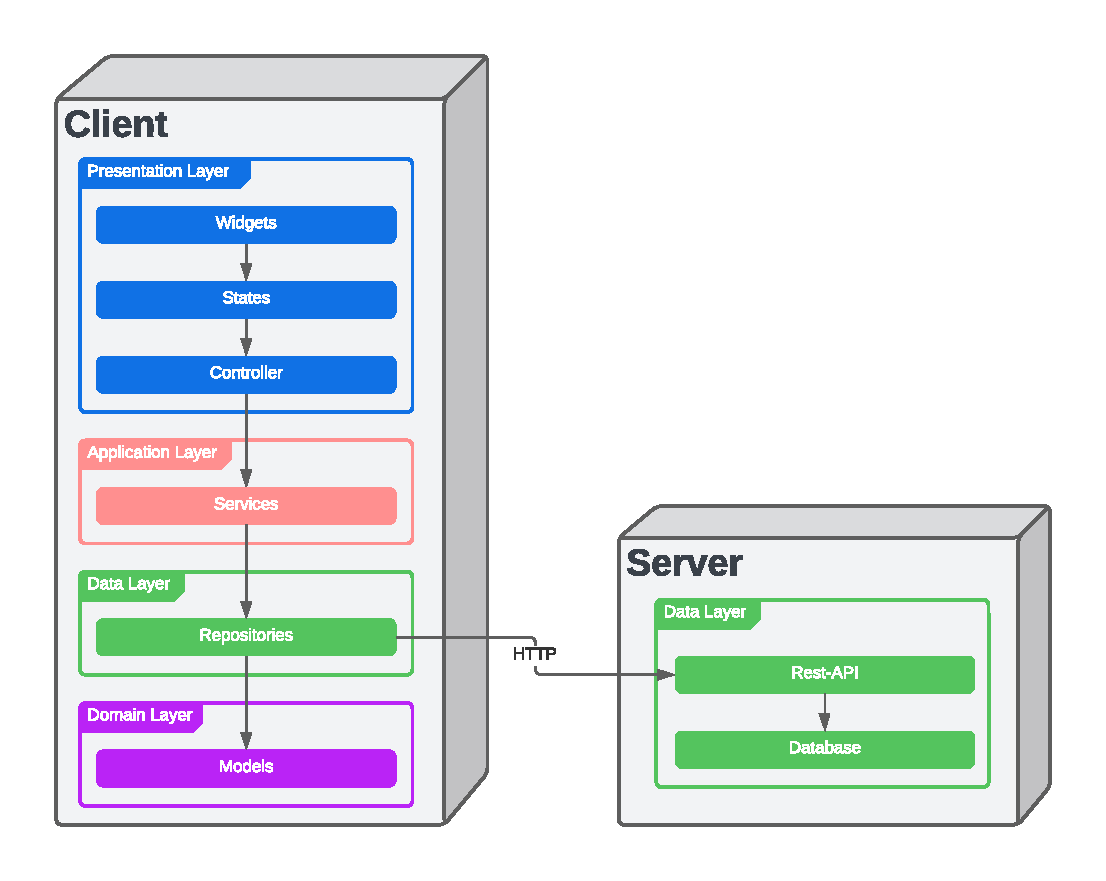
\includegraphics[height = 0.4\textheight]{images/architecture/architecture.pdf}
    \caption{Architektur der Applikation}
    \label{fig:struktur}
\end{figure}

Die Pfeile in der Grafik bedeutet die Richtung der Abhängigkeiten. So kann beispielsweise der Presentation Layer auf den Application Layer zugreifen, aber nicht umgekehrt. Der Presentation Layer dürfte aber auch auf den Data Layer zugreifen. Der Server wird nur von den Repositories über HTTP-Anfragen angesprochen.
Die einzelnen Schichten werden in den folgenden Kapiteln genauer beschrieben.
\newpage

\section{Domain Layer}
Der Domain Layer enthält in erster Linie die Models der einzelnen Entitäten. Diese sollen nun genauer beschrieben werden. In den folgenden Klassendiagrammen wurden Getter der Übersicht halber weggelassen. Sie werden jedoch immer im Text beschrieben, sofern es sie gibt.
\begin{figure}[htp]
    \centering
    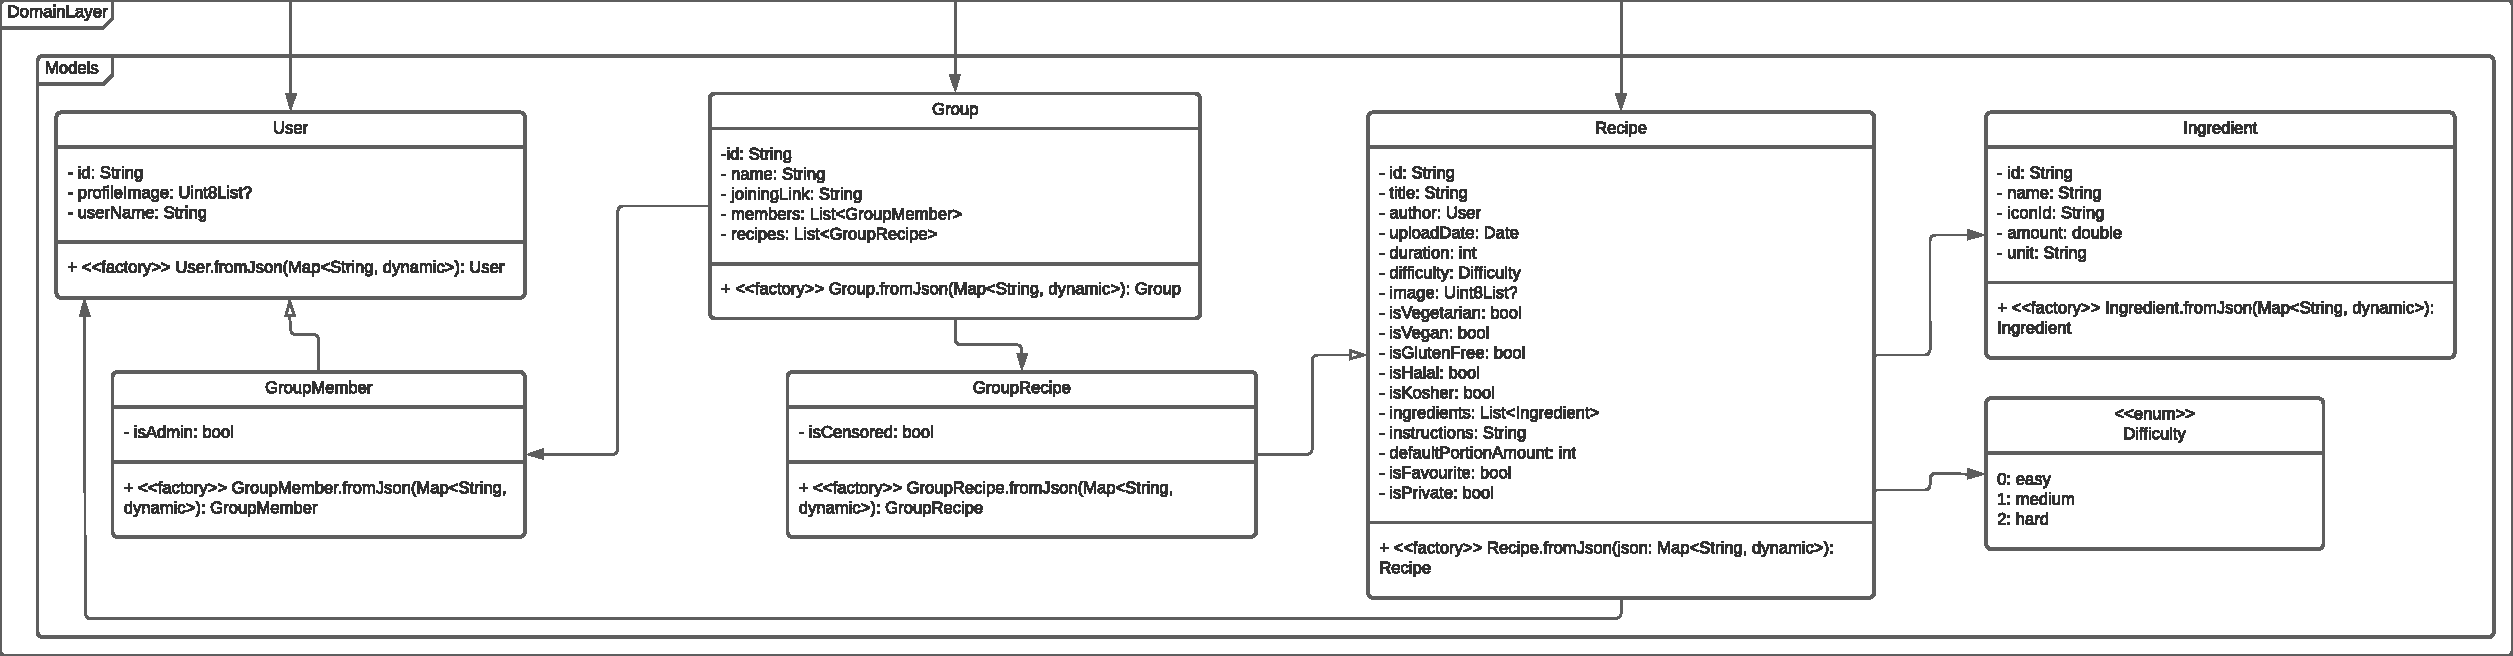
\includegraphics[width = \textwidth]{images/domainLayer/domainLayer.pdf}
    \caption{Klassendiagramm der Model-Klassen}
    \label{fig:domain-layer}
\end{figure}
\newpage
\subsection{\texttt{User}}\label{sec:User}
Die Klasse \texttt{User} repräsentiert einen Nutzer der App.
\subsubsection*{Attribute}
Alle Attribute sind privat und können nur über einen Getter gelesen werden.
\paragraph{\texttt{id: String}}
Die eindeutige ID des Nutzers. Diese wird vom Server vergeben und ist somit nicht vom Nutzer selbst zu setzen.
\paragraph{\texttt{profileImage: Uint8List?}}
Das Profilbild des Nutzers. Der Typ \texttt{Uint8List} ist ein Array von Bytes, welches das Bild in binärer Form enthält. Dieses Attribut ist optional, da nicht jeder Nutzer ein Profilbild haben muss.
\paragraph{\texttt{username: String}}
Der Nutzername des Nutzers.

\subsubsection*{Methoden}
\paragraph{\texttt{getId(): String}}
Gibt die ID des Nutzers zurück.
\paragraph{\texttt{getProfileImage(): Uint8List?}}
Gibt das Profilbild des Nutzers zurück. Ist kein Profilbild gesetzt, wird null zurückgegeben.
\paragraph{\texttt{getUsername(): String}}
Gibt den Nutzernamen des Nutzers zurück.
\paragraph{\texttt{factory User.fromJson(Map<String, dynamic> json): User}} Factory-Methode, die dazu dient, ein \texttt{User}-Objekt aus einem \glslink{JSON}{JSON-Objekt} zu erstellen. Sie wird verwendet, um die Daten, die vom Server geschickt werden und in \Gls{JSON} vorliegen, in ein \texttt{User}-Objekt umzuwandeln. Die Methode ist statisch, da sie kein \texttt{User}-Objekt benötigt, um aufgerufen zu werden. Nimmt als Parameter das bereits in eine Map umgewandelte \glslink{JSON}{JSON-Objekt} entgegen und gibt ein \texttt{User}-Objekt zurück.
\newpage

\subsection{\texttt{Recipe}}\label{sec:Recipe}
Die Klasse \texttt{Recipe} repräsentiert ein Rezept.
\subsubsection*{Attribute}
Alle Attribute sind privat und können nur über Getter-Methoden abgerufen werden.
\paragraph{\texttt{id: String}}
Die eindeutige ID des Rezepts. Diese wird vom Server vergeben und ist somit nicht vom Nutzer selbst zu setzen.
\paragraph{\texttt{title: String}}
Der Titel des Rezepts.
\paragraph{\texttt{author: User}}
Der Autor des Rezepts.
\paragraph{\texttt{uploadDate: Date}}
Das Datum, an dem das Rezept hochgeladen wurde.
\paragraph{\texttt{duration: int}}
Die Dauer zum Nachkochen des Rezepts in Minuten.
\paragraph{\texttt{difficulty: Difficulty}}
Die Schwierigkeit des Rezepts.
\paragraph{\texttt{image: Uint8List?}}
Das Bild des Rezepts. Der Typ Uint8List ist ein Array von Bytes, welches das Bild in binärer Form enthält. Dieses Attribut ist optional, da nicht jedes Rezept ein Bild haben muss.
\paragraph{\texttt{isVegetartian: bool}}
Gibt an, ob das Label "Vegetarisch" aktiviert ist.
\paragraph{\texttt{isVegan: bool}}
Gibt an, ob das Label "Vegan" aktiviert ist.
\paragraph{\texttt{isGlutenFree: bool}}
Gibt an, ob das Label "Glutenfrei" aktiviert ist.
\paragraph{\texttt{isHalal: bool}}
Gibt an, ob das Label "Halal" aktiviert ist.
\paragraph{\texttt{isKosher: bool}}
Gibt an, ob das Label "Koscher" aktiviert ist.
\paragraph{\texttt{ingredients: List<Ingredient>}}
Die Liste der Zutaten, die für das Rezept benötigt werden.
\paragraph{\texttt{instructions: String}}
Die Zubereitungsanleitung des Rezepts.
\paragraph{\texttt{defaultPortionAmount: int}}
Die Anzahl der Portionen, die das Rezept standardmäßig ergibt. Wird zum Berechnen der Mengen der Zutaten benötigt.
\paragraph{\texttt{isFavourite: bool}}
Gibt an, ob das Rezept vom Nutzer als Favorit markiert wurde.
\paragraph{\texttt{isPrivate: bool}}
Gibt an, ob das Rezept privat ist. Private Rezepte können nur vom Autor selbst gesehen werden.

\subsubsection*{Methoden}
\paragraph{\texttt{getId(): String}}
Gibt die ID des Rezepts zurück.
\paragraph{\texttt{getTitle(): String}}
Gibt den Titel des Rezepts zurück.
\paragraph{\texttt{getAuthor(): User}}
Gibt den Autor des Rezepts zurück.
\paragraph{\texttt{getUploadDate(): Date}}
Gibt das Datum, an dem das Rezept hochgeladen wurde, zurück.
\paragraph{\texttt{getDuration(): int}}
Gibt die Dauer zum Nachkochen des Rezepts in Minuten zurück.
\paragraph{\texttt{getDifficulty(): Difficulty}}
Gibt die Schwierigkeit des Rezepts zurück.
\paragraph{\texttt{getImage(): Uint8List?}}
Gibt das Bild des Rezepts zurück. Ist kein Bild gesetzt, wird null zurückgegeben.
\paragraph{\texttt{getIsVegetarian(): bool}}
Gibt zurück, ob das Label "Vegetarisch" aktiviert ist.
\paragraph{\texttt{getIsVegan(): bool}}
Gibt zurück, ob das Label "Vegan" aktiviert ist.
\paragraph{\texttt{getIsGlutenFree(): bool}}
Gibt zurück, ob das Label "Glutenfrei" aktiviert ist.
\paragraph{\texttt{getIsHalal(): bool}}
Gibt zurück, ob das Label "Halal" aktiviert ist.
\paragraph{\texttt{getIsKosher(): bool}}
Gibt zurück, ob das Label "Koscher" aktiviert ist.
\paragraph{\texttt{getIngredients(): List<Ingredient>}}
Gibt die Liste der Zutaten, die für das Rezept benötigt werden, zurück.
\paragraph{\texttt{getInstructions(): String}}
Gibt die Zubereitungsanleitung des Rezepts zurück.
\paragraph{\texttt{getDefaultPortionAmount(): int}}
Gibt die Anzahl der Portionen, die das Rezept standardmäßig ergibt, zurück.
\paragraph{\texttt{getIsFavourite(): bool}}
Gibt zurück, ob das Rezept vom Nutzer als Favorit markiert wurde.
\paragraph{\texttt{getIsPrivate(): bool}}
Gibt zurück, ob das Rezept privat ist.
\paragraph{\texttt{factory Recipe.fromJson(Map<String, dynamic> json): Recipe}}
Es handelt sich um eine Factory-Methode, die \texttt{Recipe}-Objekte aus \glslink{JSON}{JSON-Objekten} erstellen kann. Sie wird verwendet, um die Daten, die vom Server geschickt werden und in \Gls{JSON} vorliegen, in ein \texttt{Recipe}-Objekt umzuwandeln. Die Methode ist statisch, da sie kein \texttt{Recipe}-Objekt benötigt, um aufgerufen zu werden. Nimmt als Parameter das bereits in eine Map umgewandelte \glslink{JSON}{JSON-Objekt} entgegen und gibt ein \texttt{Recipe}-Objekt zurück.

\newpage
\subsection{\texttt{Ingredient}}\label{sec:ingredient}
Die Klasse \texttt{Ingredient} repräsentiert eine Zutat, die einem Rezept zugeordnet ist.
\subsubsection*{Attribute}
Alle Attribute sind privat und können nur über Getter-Methoden abgerufen werden.
\paragraph{\texttt{id: String}}
Die eindeutige ID der Zutat. Diese wird vom Server vergeben und ist somit nicht vom Nutzer selbst zu setzen.
\paragraph{\texttt{name: String}}
Der Name der Zutat.
\paragraph{\texttt{iconId: String}}
Die Id des Icons, das der Zutat zugeordnet ist.
\paragraph{\texttt{amount: double}}
Die Menge der Zutat, die für das Rezept benötigt wird.
\paragraph{\texttt{unit: String}}
Die Einheit der Zutatenmenge.

\subsubsection*{Methoden}
\paragraph{\texttt{getId(): String}}
Gibt die ID der Zutat zurück.
\paragraph{\texttt{getName(): String}}
Gibt den Namen der Zutat zurück.
\paragraph{\texttt{getIconId(): String}}
Gibt die Id des Icons, das der Zutat zugeordnet ist, zurück.
\paragraph{\texttt{getAmount(): double}}
Gibt die Menge der Zutat, die für das Rezept benötigt wird, zurück.
\paragraph{\texttt{getUnit(): String}}
Gibt die Einheit der Zutatenmenge zurück.
\paragraph{\texttt{factory Ingredient.fromJson(Map<String, dynamic> json): Ingredient}}
Dies ist eine Factory-Methode zum Erstellen eines \texttt{Ingredient}-Objekts aus einem \glslink{JSON}{JSON-Objekt}. Sie wird verwendet, um die Daten, die vom Server geschickt werden und in \Gls{JSON} vorliegen, in ein \texttt{Ingredient}-Objekt umzuwandeln. Die Methode ist statisch, da sie kein \texttt{Ingredient}-Objekt benötigt, um aufgerufen zu werden. Nimmt als Parameter das bereits in eine Map umgewandelte \glslink{JSON}{JSON-Objekt} entgegen und gibt ein \texttt{Ingredient}-Objekt zurück.

\newpage
\subsection{\texttt{Difficulty}}\label{sec:difficulty}
Der Enum \texttt{Difficulty} repräsentiert die Schwierigkeit eines Rezepts. Er kann folgende Werte annehmen:
\begin{itemize}
    \item \texttt{EASY}
    \item \texttt{MEDIUM}
    \item \texttt{HARD}
\end{itemize}
\newpage

\subsection{\texttt{Group}}\label{sec:group}
Die Klasse \texttt{Group} repräsentiert eine Gruppe bzw. Squad von Nutzern.
\subsubsection*{Attribute}
Alle Attribute sind privat und können nur über einen Getter gelesen werden.
\paragraph{\texttt{id: String}}
Die eindeutige ID der Gruppe. Diese wird vom Server vergeben und ist somit nicht vom Nutzer selbst zu setzen.
\paragraph{\texttt{name: String}}
Der Name der Gruppe.
\paragraph{\texttt{joiningLink: String}}
Das Gruppenkürzel der Gruppe. Es wird verwendet, um einer Gruppe beizutreten.
\paragraph{\texttt{members: List<GroupMember>}}
Die Liste der Mitglieder der Gruppe. Die Liste ist nicht leer, da eine Gruppe mindestens einen Nutzer enthalten muss.
\paragraph{\texttt{recipes: List<GroupRecipe>}}
Die Liste der Rezepte, die von Mitgliedern der Gruppe erstellt wurden.

\subsubsection*{Methoden}
\paragraph{\texttt{getId(): String}}
Gibt die ID der Gruppe zurück.
\paragraph{\texttt{getName(): String}}
Gibt den Namen der Gruppe zurück.
\paragraph{\texttt{getJoiningLink(): String}}
Gibt das Gruppenkürzel der Gruppe zurück.
\paragraph{\texttt{getMembers(): List<GroupMember>}}
Gibt die Liste der Mitglieder der Gruppe zurück.
\paragraph{\texttt{getRecipes(): List<GroupRecipe>}}
Gibt die Liste der Rezepte der Gruppe zurück.
\paragraph{\texttt{factory Group.fromJson(Map<String, dynamic> json): Group}} Factory-Methode zur Erstellung eines \texttt{Group}-Objekts aus einem \glslink{JSON}{JSON-Objekt}. Sie wird verwendet, um die Daten, die vom Server geschickt werden und in \Gls{JSON} vorliegen, in ein \texttt{Group}-Objekt umzuwandeln. Die Methode ist statisch, da sie kein \texttt{Group}-Objekt benötigt, um aufgerufen zu werden. Nimmt als Parameter das bereits in eine Map umgewandelte \glslink{JSON}{JSON-Objekt} entgegen und gibt ein \texttt{Group}-Objekt zurück.

\newpage
\subsection{\texttt{GroupMember}}\label{sec:GroupMember}
Die Klasse \texttt{GroupMember} repräsentiert ein Mitglied einer Gruppe. Sie erbt von der Klasse \texttt{User}.
\subsubsection*{Attribute}
Alle Attribute sind privat und können nur über einen Getter gelesen werden.
\paragraph{\texttt{isAdmin: bool}}
Gibt an, ob das Mitglied Administrator der Gruppe, der es zugeordnet ist, ist.
\subsubsection*{Methoden}
\paragraph{\texttt{getIsAdmin(): bool}}
Gibt zurück, ob das Mitglied Administrator der Gruppe, der es zugeordnet ist, ist.
\paragraph{\texttt{factory GroupMember.fromJson(Map<String, dynamic> json): GroupMember}} Es handelt sich um eine Factory-Methode zum Erstellen eines \texttt{GroupMember}-Objekts aus einem \glslink{JSON}{JSON-Objekt}. Sie wird verwendet, um die Daten, die vom Server geschickt werden und in \Gls{JSON} vorliegen, in ein \texttt{GroupMember}-Objekt umzuwandeln. Die Methode ist statisch, da sie kein \texttt{GroupMember}-Objekt benötigt, um aufgerufen zu werden. Nimmt als Parameter das bereits in eine \Gls{map} umgewandelte \glslink{JSON}{JSON-Objekt} entgegen und gibt ein \texttt{GroupMember}-Objekt zurück.
\newpage
\subsection{\texttt{GroupRecipe}}\label{sec:GroupRecipe}
Die Klasse \texttt{GroupRecipe} repräsentiert ein Rezept, das einer konkreten Gruppe zugeordnet wurde. Sie erbt von der Klasse \texttt{Recipe}.
\subsubsection*{Attribute}
Alle Attribute sind privat und können nur über einen Getter gelesen werden.
\paragraph{\texttt{isCensored: bool}}
Gibt an, ob das Rezept von einem Administrator der Gruppe zensiert wurde.
\subsubsection*{Methoden}
\paragraph{\texttt{getIsCensored(): bool}}
Gibt zurück, ob das Rezept von einem Administrator der Gruppe zensiert wurde.
\paragraph{\texttt{factory GroupRecipe.fromJson(Map<String, dynamic> json): GroupRecipe}} Es handelt sich um eine Factory-Methode zum Erstellen eines \texttt{GroupRecipe}-Objekts aus einem \glslink{JSON}{JSON-Objekt}. Sie wird verwendet, um die Daten, die vom Server geschickt werden und in \Gls{JSON} vorliegen, in ein \texttt{GroupRecipe}-Objekt umzuwandeln. Die Methode ist statisch, da sie kein \texttt{GroupRecipe}-Objekt benötigt, um aufgerufen zu werden. Nimmt als Parameter das bereits in eine \Gls{map} umgewandelte \glslink{JSON}{JSON-Objekt} entgegen und gibt ein \texttt{GroupRecipe}-Objekt zurück.

\newpage
\section{Data Layer}
Der Data Layer ist für die Datenverarbeitung und -verwaltung verantwortlich. In der App selbst befinden sich lediglich die Repository-Klassen. Sie fungieren als eine Abstraktionsebene zwischen der Geschäftslogik (Application Layer) und den Datenquellen, wie z. B. einer lokalen Datenbank oder einem Remote-Server. Die Repository-Klassen bieten eine Schnittstelle, über die die Geschäftslogik auf die Daten zugreifen kann, ohne Details über deren Speicherung oder Beschaffung zu kennen. Sie bieten Methoden zur Datenabfrage, -aktualisierung und -speicherung und handhaben die Kommunikation mit den entsprechenden Datenquellen. Dadurch wird eine lose Kopplung zwischen der Geschäftslogik und den konkreten Datenquellen erreicht und ermöglicht eine flexiblere Handhabung von Datenquellenwechseln oder -aktualisierungen. Repository-Klassen unterstützen auch das Prinzip der Datenkapselung und fördern eine saubere und modularisierte Architektur in der App-Entwicklung.
Nun sollen die einzelnen Repository-Klassen vorgestellt werden. Die Klassen sind in der Abbildung dargestellt.
\begin{figure}[htp]
    \centering
    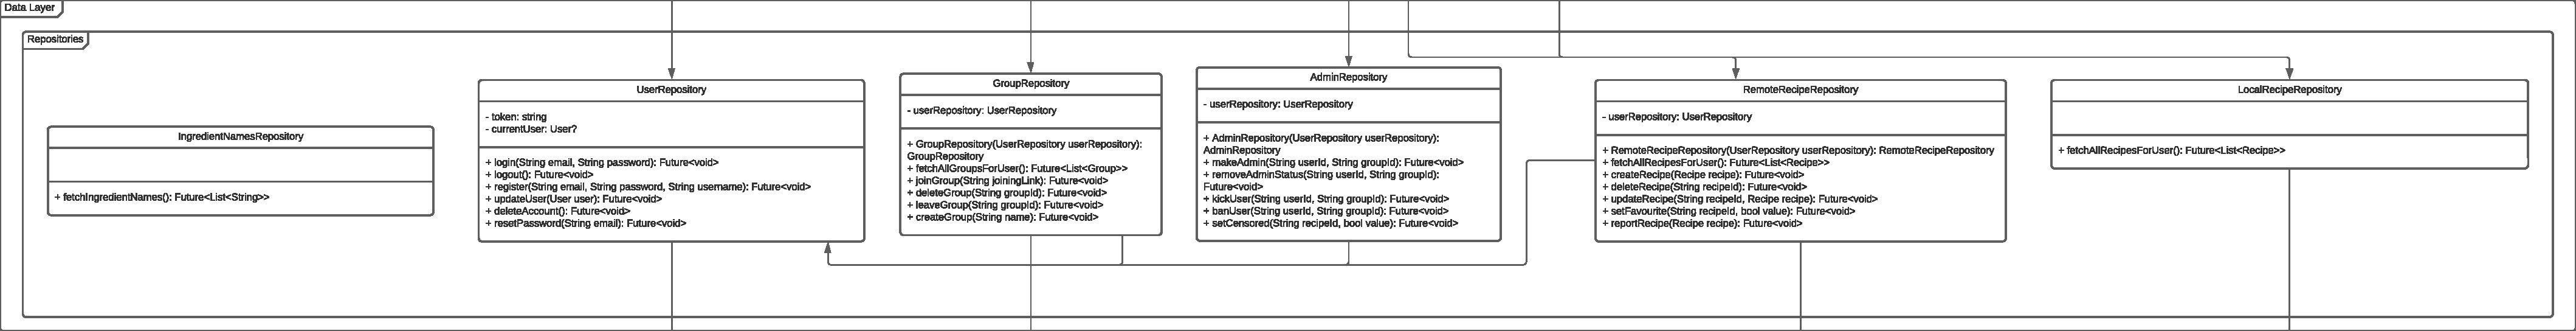
\includegraphics[width=\textwidth]{images/dataLayer/dataLayer.pdf}
    \caption{Klassendiagramm der Repository-Klassen}
    \label{fig:dataLayer}
\end{figure}
\newpage
\subsection{\texttt{UserRepository}}\label{sec:UserRepository}
Das \texttt{UserRepository} stellt die Schnittstelle zwischen der Geschäftslogik und der Datenquelle für Nutzer dar. Es bietet Methoden zur Abfrage, Aktualisierung und Speicherung von Nutzern speichert das Token zur Authentifizierung des Nutzers bei dem Server.
\subsubsection*{Attribute}
\paragraph{\texttt{token: String}}
Das Token zur Authentifizierung des Nutzers mit dem Server. Es handelt sich um ein privates Attribut, das nur über einen Getter gelesen werden kann. Das Token entspricht dem JWT-Token, das der Server nach der Authentifizierung des Nutzers zurückgibt. Darin sind unteranderem die Nutzer-ID und die Gültigkeitsdauer des Tokens kodiert enthalten.
\paragraph{\texttt{currentUser: User}}
Das \texttt{User}-Objekt, das den aktuell angemeldeten Nutzer repräsentiert. Es handelt sich um ein privates Attribut, das nur über einen Getter gelesen werden kann.
\subsubsection*{Methoden}
\paragraph{\texttt{getToken(): String}}
Gibt das Token zur Authentifizierung des Nutzers bei dem Server zurück.
\paragraph{\texttt{getCurrentUser(): User}}
Gibt das \texttt{User}-Objekt, das den aktuell angemeldeten Nutzer repräsentiert, zurück.
\paragraph{\texttt{login(String email, String password): Future<void>}}
Es wird eine Anfrage zum Nutzer Anmelden an den Server gestellt. Nimmt als Parameter die E-Mail-Adresse und das Passwort des Nutzers entgegen. Die Methode ist asynchron und gibt ein \texttt{Future}-Objekt zurück. Das \texttt{Future}-Objekt wird aufgelöst, wenn die Anmeldung erfolgreich war. Wenn die Anmeldung fehlschlägt, wird eine Exception geworfen. Die Methode speichert das Token in dem privaten Attribut \texttt{token} und das \texttt{User}-Objekt, das den aktuell angemeldeten Nutzer repräsentiert, in dem privaten Attribut \texttt{currentUser}.
\paragraph{\texttt{logout(): Future<void>}}
Es wird eine Anfrage an den Server zum Abmelden des Nutzers gestellt. Die Methode ist asynchron und gibt ein \texttt{Future}-Objekt zurück. Das \texttt{Future}-Objekt wird aufgelöst, wenn die Abmeldung erfolgreich war. Wenn die Abmeldung fehlschlägt, wird eine Exception geworfen. Die Methode löscht das Token aus dem privaten Attribut \texttt{token} und das \texttt{User}-Objekt aus dem privaten Attribut \texttt{currentUser}.
\paragraph{\texttt{register(String email, String password, String username): Future<void>}}
Stellt eine Anfrage an den Server, einen neuen Nutzer zu registrieren. Nimmt als Parameter die E-Mail-Adresse, das Passwort und den Nutzernamen des Nutzers entgegen. Die Methode ist asynchron und gibt ein \texttt{Futur}-Objekt zurück. Das \texttt{Future}-Objekt wird aufgelöst, wenn die Registrierung erfolgreich war. Wenn die Registrierung fehlschlägt, wird eine Exception geworfen. Die Methode speichert das Token in dem privaten Attribut \texttt{token} und das \texttt{User}-Objekt, das den aktuell angemeldeten Nutzer repräsentiert, in dem privaten Attribut \texttt{currentUser}.
\paragraph{\texttt{updateUser(User user): Future<void>}}
Es wird eine Anfrage an den Server gesendet, den angemeldeten Nutzer zu aktualisieren. Die Methode aktualisiert das \texttt{User}-Objekt, das den aktuell angemeldeten Nutzer repräsentiert, in dem privaten Attribut \texttt{currentUser}.
Die Methode ist asynchron und gibt ein \texttt{Future}-Objekt zurück. Das \texttt{Future}-Objekt wird aufgelöst, wenn die Anfrage erfolgreich war. Wenn die Anfrage fehlschlägt, wird eine Exception geworfen.
\paragraph{deleteAccount(): Future<void>}
Es wird eine Anfrage an den Server gesendet, um den Account des aktuell angemeldeten Nutzers zu löschen. Die Methode ist asynchron und gibt ein \texttt{Future}-Objekt zurück. Das \texttt{Future}-Objekt wird aufgelöst, wenn die Anfrage erfolgreich war. Wenn die Anfrage fehlschlägt, wird eine Exception geworfen. Die Methode führt im Anschluss die Methode \texttt{logout()} aus.
\paragraph{resetPassword(String email): Future<void>}
Es wird eine Anfrage an den Server zum Zurücksetzen des Passworts gesendet. Nimmt als Parameter die E-Mail-Adresse des Nutzers entgegen. Die Methode ist asynchron und gibt ein \texttt{Future}-Objekt zurück. Das \texttt{Future}-Objekt wird aufgelöst, wenn der Server eine E-Mail zum Zurücksetzen des Passworts versendet hat. Wenn das Versenden fehlschlägt, wird eine Exception geworfen.

\newpage
\subsection{\texttt{GroupRepository}}\label{sec:GroupRepository}
Das \texttt{GroupRepository} stellt die Schnittstelle zwischen der Geschäftslogik und der Datenquelle für Gruppen dar. Es bietet Methoden zur Abfrage, Aktualisierung und Speicherung von Gruppen.
\subsubsection*{Attribute}
\paragraph{\texttt{userRepository: UserRepository}}
\texttt{UserRepository}-Objekt, welches das \texttt{GroupRepository}-Objekt verwendet. Es handelt sich um ein privates Attribut. Es wird später verwendet, um das Token zur Authentifizierung des Nutzers bei dem Server für Anfragen zu erhalten.
\subsubsection*{Methoden}
\paragraph{\texttt{GroupRepository(UserRepository userRepository): GroupRepository}}
Konstruktor. Initialisiert das Attribut \texttt{userRepository} mit dem übergebenen \texttt{UserRepository}-Objekt.
\paragraph{\texttt{fetchAllGroupsForUser(): Future<List<Group>>}}
Fragt alle Gruppen des aktuellen Nutzers beim Server ab und gibt diese als Liste zurück. Die Methode ist asynchron und gibt ein \texttt{Future}-Objekt zurück. Das \texttt{Future}-Objekt wird aufgelöst, wenn die Abfrage erfolgreich war. Wenn die Abfrage fehlschlägt, wird eine Exception geworfen.
\paragraph{\texttt{joinGroup(String joiningLink): Future<void>}}
Es wird eine Anfrage an den Server zum Beitritt des aktuellen Nutzers zu einer Gruppe mit dem übergebenen Beitrittslink gestellt. Nimmt als Parameter den Beitrittslink der Gruppe entgegen. Die Methode ist asynchron und gibt ein \texttt{Future}-Objekt zurück. Das \texttt{Future}-Objekt wird aufgelöst, wenn der Nutzer erfolgreich der Gruppe beigetreten ist. Wenn der Nutzer der Gruppe nicht beitreten kann, wird eine Exception geworfen.
\paragraph{\texttt{deleteGroup(String groupId): Future<void>}}
Es wird eine Anfrage an den Server zum Löschen einer Gruppe mit der übergebenen Gruppen-ID gestellt. Nimmt als Parameter die ID der Gruppe entgegen. Die Methode ist asynchron und gibt ein \texttt{Future}-Objekt zurück. Das \texttt{Future}-Objekt wird aufgelöst, wenn die Gruppe erfolgreich gelöscht wurde. Wenn die Gruppe nicht gelöscht werden kann, wird eine Exception geworfen.
\paragraph{\texttt{leaveGroup(String groupId): Future<void>}}
Es wird eine Anfrage an den Server zum Austritt des aktuellen Nutzers aus einer Gruppe mit der übergebenen Gruppen-ID gestellt. Nimmt als Parameter die ID der Gruppe entgegen. Die Methode ist asynchron und gibt ein \texttt{Future}-Objekt zurück. Das \texttt{Future}-Objekt wird aufgelöst, wenn der Nutzer erfolgreich die Gruppe verlassen hat. Wenn der Nutzer die Gruppe nicht verlassen kann, wird eine Exception geworfen.
\paragraph{\texttt{createGroup(String name): Future<void>}}
Es wird eine Anfrage an den Server zum Erstellen einer neuen Gruppe mit dem übergebenen Namen gestellt. Nimmt als Parameter den Namen der Gruppe entgegen. Die Methode ist asynchron und gibt ein \texttt{Future}-Objekt zurück. Das \texttt{Future}-Objekt wird aufgelöst, wenn die Gruppe erfolgreich erstellt wurde. Wenn die Gruppe nicht erstellt werden kann, wird eine Exception geworfen.

\newpage
\subsection{\texttt{AdminRepository}}\label{sec:AdminRepository}
Das \texttt{AdminRepository} stellt die Schnittstelle zwischen der Geschäftslogik und den Server-Schnittstellen für verschiedene Administratoraktionen dar.
\subsubsection*{Attribute}
\paragraph{\texttt{userRepository: UserRepository}}
\texttt{UserRepository}-Objekt, welches das \texttt{AdminRepository}-Objekt verwendet. Es handelt sich um ein privates Attribut. Es wird später verwendet, um das Token zur Authentifizierung des Nutzers bei dem Server für Anfragen zu erhalten.
\subsubsection*{Methoden}
\paragraph{\texttt{AdminRepository(UserRepository userRepository): AdminRepository}}
Konstruktor. Initialisiert das Attribut \texttt{userRepository} mit dem übergebenen \texttt{UserRepository}-Objekt.
\paragraph{\texttt{makeAdmin(String userId, String groupId): Future<void>}}
Es wird eine Anfrage an den Server gestellt, um den Nutzer mit der übergebenen ID zum Administrator der Gruppe mit der übergebenen ID zu machen. Nimmt als Parameter die ID des Nutzers und die ID der Gruppe entgegen. Die Methode ist asynchron und gibt ein \texttt{Future}-Objekt zurück. Das \texttt{Future}-Objekt wird aufgelöst, wenn der Nutzer erfolgreich zum Administrator der Gruppe gemacht wurde. Wenn der Nutzer nicht zum Administrator der Gruppe gemacht werden kann, wird eine Exception geworfen.

\paragraph{\texttt{removeAdminStatus(String userId, String groupId): Future<void>}}
Es wird eine Anfrage an den Server gestellt, um den Nutzer mit der übergebenen ID den Administratorstatus der Gruppe mit der übergebenen ID zu entziehen. Nimmt als Parameter die ID des Nutzers und die ID der Gruppe entgegen. Die Methode ist asynchron und gibt ein \texttt{Future}-Objekt zurück. Das \texttt{Future}-Objekt wird aufgelöst, wenn der Nutzer erfolgreich den Administratorstatus der Gruppe entzogen bekommen hat. Wenn der Nutzer nicht den Administratorstatus der Gruppe entzogen bekommen kann, wird eine Exception geworfen.
\paragraph{\texttt{kickUser(String userId, String groupId): Future<void>}}
Es wird eine Anfrage an den Server gestellt, um den Nutzer mit der übergebenen ID aus der Gruppe mit der übergebenen ID zu entfernen. Nimmt als Parameter die ID des Nutzers und die ID der Gruppe entgegen. Die Methode ist asynchron und gibt ein \texttt{Future}-Objekt zurück. Das \texttt{Future}-Objekt wird aufgelöst, wenn der Nutzer erfolgreich aus der Gruppe entfernt wurde. Wenn der Nutzer nicht aus der Gruppe entfernt werden kann, wird eine Exception geworfen.
\paragraph{\texttt{banUser(String userId, String groupId): Future<void>}}
Es wird eine Anfrage an den Server gestellt, um den Nutzer mit der übergebenen ID aus der Gruppe mit der übergebenen ID zu bannen. Nimmt als Parameter die ID des Nutzers und die ID der Gruppe entgegen. Die Methode ist asynchron und gibt ein \texttt{Future}-Objekt zurück. Das \texttt{Future}-Objekt wird aufgelöst, wenn der Nutzer erfolgreich aus der Gruppe gebannt wurde. Wenn der Nutzer nicht aus der Gruppe gebannt werden kann, wird eine Exception geworfen.
\paragraph{\texttt{setCensored(String recipeId, bool value): Future<void>}}
Zensiert das Rezept, das die gegebene ID besitzt. Nimmt als Parameter die ID des Rezepts und einen boolschen Wert, der angibt, ob das Rezept als zensiert gesetzt oder entfernt werden soll, entgegen. Die Methode ist asynchron und gibt ein \texttt{Future}-Objekt zurück. Das \texttt{Future}-Objekt wird aufgelöst, wenn das Rezept erfolgreich als zensiert gesetzt oder entfernt wurde. Wenn das Rezept nicht als zensiert gesetzt oder entfernt werden kann, wird eine Exception geworfen.
\newpage
\subsection{\texttt{RemoteRecipeRepository}}\label{sec:RemoteRecipeRepository}
Das \texttt{RemoteRecipeRepository} stellt die Schnittstelle zwischen der Geschäftslogik und den Server-Schnittstellen für Rezepte dar.
\subsubsection*{Attribute}
\paragraph{\texttt{userRepository: UserRepository}}
Das \texttt{UserRepository}-Objekt, welches von dem \texttt{Remote\-Recipe\-Repository}-Objekt verwendet wird. Es handelt sich um ein privates Attribut. Es wird später verwendet, um das Token zur Authentifizierung des Nutzers bei dem Server für Anfragen zu erhalten.
\subsubsection*{Methoden}
\paragraph{\texttt{RemoteRecipeRepository(UserRepository userRepository):RemoteRecipeRepository\\}}
Der Konstruktor der Klasse. Initialisiert das Attribut \texttt{userRepository} mit dem übergebenen \texttt{UserRepository}-Objekt.
\paragraph{\texttt{fetchAllRecipesForUser(): Future<List<Recipe>>}}
Fragt alle Rezepte aus Gruppen des aktuellen Nutzers vom Server ab. Nimmt keine Parameter entgegen. Die Methode ist asynchron und gibt ein \texttt{Future}-Objekt zurück. Das \texttt{Future}-Objekt wird aufgelöst, wenn die Rezepte erfolgreich vom Server abgefragt wurden. Wenn die Rezepte nicht vom Server abgefragt werden können, wird eine Exception geworfen. Speichert zudem alle Rezepte als JSON-Objekt via \Gls{SharedPreferences} in den lokalen Speicher.
\paragraph{\texttt{createRecipe(Recipe recipe): Future<void>}}
Erstellt ein neues Rezept auf dem Server. Nimmt als Parameter das Rezept, das erstellt werden soll, entgegen. Die Methode ist asynchron und gibt ein \texttt{Future}-Objekt zurück. Das \texttt{Future}-Objekt wird aufgelöst, wenn das Rezept erfolgreich erstellt wurde. Wenn das Rezept nicht erstellt werden kann, wird eine Exception geworfen.
\paragraph{\texttt{deleteRecipe(String recipeId): Future<void>}}
Löscht das Rezept mit der übergebenen ID vom Server. Nimmt als Parameter die ID des Rezepts entgegen. Die Methode ist asynchron und gibt ein \texttt{Future}-Objekt zurück. Das \texttt{Future}-Objekt wird aufgelöst, wenn das Rezept erfolgreich gelöscht wurde. Wenn das Rezept nicht gelöscht werden kann, wird eine Exception geworfen.
\paragraph{\texttt{updateRecipe(String recipeId, Recipe recipe): Future<void>}}
Ändert das Rezept mit der übergebenen ID auf dem Server. Nimmt als Parameter die ID des Rezepts und das aktualisierte Rezept entgegen. Die Methode ist asynchron und gibt ein \texttt{Future}-Objekt zurück. Das \texttt{Future}-Objekt wird aufgelöst, wenn das Rezept erfolgreich aktualisiert wurde. Wenn das Rezept nicht aktualisiert werden kann, wird eine Exception geworfen.
\paragraph{\texttt{setFavourite(String recipeId, bool value): Future<void>}}
Setzt das Rezept mit der übergebenen ID als Favorit des aktuellen Nutzers. Nimmt als Parameter die ID des Rezepts und einen boolschen Wert, der angibt, ob das Rezept als Favorit gesetzt oder entfernt werden soll, entgegen. Die Methode ist asynchron und gibt ein \texttt{Future}-Objekt zurück. Das \texttt{Future}-Objekt wird aufgelöst, wenn das Rezept erfolgreich als Favorit gesetzt oder entfernt wurde. Wenn das Rezept nicht als Favorit gesetzt oder entfernt werden kann, wird eine Exception geworfen.
\newpage
\subsection{\texttt{LocalRecipeRepository}}\label{sec:LocalRecipeRepository}
Das \texttt{LocalRecipeRepository} stellt die Schnittstelle zwischen der Geschäftslogik und dem lokalen Speicher für Rezepte dar.
\subsubsection*{Methoden}
\paragraph{\texttt{fetchAllRecipesForUser(): Future<List<Recipe>>}}
Fragt alle Rezepte aus Gruppen des aktuellen Nutzers aus dem lokalen Speicher via \Gls{SharedPreferences} ab. Nimmt keine Parameter entgegen. Die Methode ist asynchron und gibt ein \texttt{Future}-Objekt zurück. Das \texttt{Future}-Objekt wird aufgelöst, wenn die Rezepte erfolgreich aus dem lokalen Speicher abgefragt wurden. Wenn die Rezepte nicht aus dem lokalen Speicher abgefragt werden können, wird eine Exception geworfen.
\newpage
\section{Riverpod und Provider}
\label{sec:riverpod}
\subsection{Riverpod}
Der Sinn von Riverpod liegt darin, die Verwaltung von Zuständen und Abhängigkeiten in Flutter-Apps zu vereinfachen. Riverpod ist eine leistungsstarke und benutzerfreundliche State-Management-Bibliothek, die auf dem Konzept von "Provider" basiert. Mit Riverpod können Entwickler effizient und flexibel Zustände verwalten, Dienste bereitstellen und Abhängigkeiten zwischen verschiedenen Teilen der App verknüpfen. Dies erleichtert die Skalierbarkeit, Wiederverwendbarkeit und Testbarkeit von Flutter-Apps, da der Code klar strukturiert ist und das Trennen von Zuständen und UI-Logik erleichtert wird. Riverpod bietet eine intuitive Syntax, unterstützt einen deklarativen Ansatz zur Definition von Providern und ermöglicht das einfache Aktualisieren von Zuständen durch Nutzung des \glslink{Observer}{Observer-Konzepts}. Insgesamt erleichtert Riverpod die Entwicklung von Flutter-Apps und trägt dazu bei, den Code sauberer, wartbarer und effizienter zu gestalten.
\subsection{Provider}
Provider sind spezielle Objekte, die dazu dienen, Werte oder Abhängigkeiten in Flutter-Apps bereitzustellen. Sie fungieren als eine Art Container, der den Zugriff auf diese Werte oder Dienste innerhalb der App ermöglicht.

Es gibt viele verschiedene Arten von Providern, die für verschiedene Zwecke verwendet werden können. In der Applikation werden die folgenden Provider-Arten verwendet:

\paragraph{\texttt{Provider}}
Der \texttt{Provider} stellt einen Wert bereit, der in der gesamten App verwendet werden kann. Dies kann beispielsweise ein Zustandswert, ein Konfigurationswert oder ein Dienstobjekt sein.

\paragraph{\texttt{AsyncNotifierProvider}}
Der \texttt{AsyncNotifierProvider} ist eine spezielle Art von Provider, der einen Zustandswert bereitstellt, der asynchron aktualisiert werden kann. Dies ist nützlich, wenn der Wert von einer asynchronen Operation abhängt, z.B. einer Datenabfrage von einer API. Durch ihn kann eine automatische Aktualisierung der Daten veranlasst werden, wenn beispielsweise eine API-Anfrage abgeschlossen wurde.

Provider werden in der Hierarchie der Flutter-Widgets platziert und können über den Widget-Tree hinweg zugänglich gemacht werden. Dadurch können sie in verschiedenen Teilen der App genutzt werden, indem sie mit dem entsprechenden Provider verbunden werden.

Die Verwendung von Providern in Riverpod ermöglicht eine saubere Trennung von Zuständen und Logik, fördert die Wiederverwendbarkeit und erleichtert das Testen von Flutter-Apps.

Es wird für jede Repository-Klasse ein eigener Provider vom Typ \texttt{Provider} erstellt. Zudem erhält jeder Service einen eigenen \texttt{AsyncNotifierProvider}. Mehr zu der Funktionsweise des \texttt{AsyncNotifierProvider} mit den Services ist in Kapitel \ref{sec:asyncNotifier} zu finden.

\newpage
\section{Application Layer}
Der Application Layer ist eine weitere wichtige Komponente einer App. Seine Hauptaufgabe besteht darin, die Geschäftslogik der Anwendung zu implementieren und die Kernfunktionalität zu verwalten. Der Application Layer enthält verschiedene Klassen und Methoden, die die Regeln und Abläufe der Anwendung definieren. Er ist unabhängig von der Benutzeroberfläche und den spezifischen Details der Datenpersistenz. Stattdessen konzentriert sich der Application Layer darauf, die Kernfunktionalität der App zu modellieren und sicherzustellen, dass diese korrekt und effizient ausgeführt wird. Dadurch wird die Wiederverwendbarkeit, Testbarkeit und Flexibilität der Anwendung verbessert. Der Application Layer fungiert als Vermittler zwischen dem Presentation Layer und dem Data Layer und ermöglicht eine saubere Trennung der Verantwortlichkeiten in der App-Architektur.
Er enthält in erster Linie viele verschiedene Services, die die verschiedenen Entitäten verwalten.
\begin{figure}[htp]
    \centering
    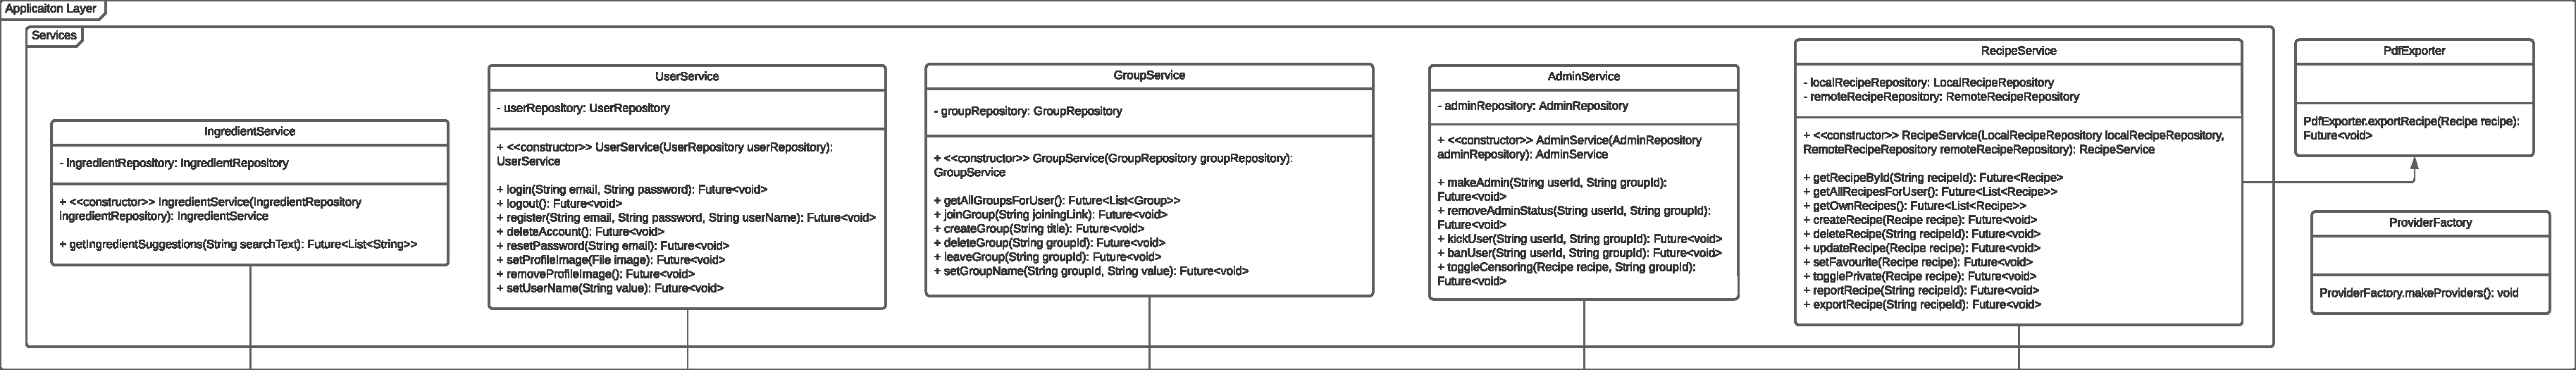
\includegraphics[width = \textwidth]{images/applicationLayer/applicationLayer.pdf}
    \caption{Klassendiagramm des Application Layer}
    \label{fig:application-layer}
\end{figure}

Nun werden die einzelnen Klassen des Application Layers beschrieben.
\newpage
\subsection{\texttt{AsyncNotifier<T>}}
\label{sec:AsyncNotifier}
Die Klasse ist Teil von Riverpod. Sie ermöglicht es Zustände asynchron zu aktualisieren. Dies ist nützlich, wenn der Wert von einer asynchronen Operation abhängt, z.B. einer Datenabfrage von einer API. Durch ihn kann eine automatische Aktualisierung der Daten veranlasst werden, wenn beispielsweise eine API-Anfrage abgeschlossen wurde.
\subsubsection*{Attribute}
\paragraph{\texttt{state: AsyncValue<T>}}
Der Zustand, der durch den \texttt{AsyncNotifier} verwaltet wird. Er ist privat und kann nur über die Methoden der Klasse geändert werden. Wird das Attribut verändert, werden alle UI-Elemente, die mit dem \texttt{AsyncNotifier} verbunden sind, infomiert und gegebenenfalls aktualisiert.
\subsubsection*{Methoden}
\paragraph{\texttt{build(): FutureOr<T>}}
Abstrakte Methode, die in den Unterklassen implementiert werden muss. Der Rückgabewert legt den Initialwert des Zustands fest.
\newpage
\subsection{\texttt{UserService}}\label{sec:UserService}
Der Service dient dazu, die Nutzer zu verwalten. Er erbt von der Klasse \texttt{AsyncNotifier<User?>}.  Das Attribut \texttt{state} enthält, immer wenn Daten verfügbar sind, den aktuellen Nutzer oder \texttt{null}, wenn kein Nutzer angemeldet ist.

\subsubsection*{Attribute}
\paragraph{\texttt{userRepository: UserRepository}}
Das \texttt{UserRepository}, das zum Zugriff auf die Nutzer verwendet wird. Es wird im Konstruktor initialisiert und ist privat.
\subsubsection*{Methoden}
\paragraph{\texttt{UserService(UserRepository userRepository): UserService}}
Konstruktor für die Klasse. Initialisiert das \texttt{UserRepository}, das zum Zugriff auf die Nutzer verwendet wird. Nimmt als Parameter das \texttt{UserRepository} entgegen.
\paragraph{\texttt{build(): FutureOr<User?>}}
Implementiert die abstrakte Methode \texttt{build()} der Klasse \texttt{Async\-Notifier}. Gibt den Initialwert des Zustands zurück. In diesem Fall ist der Initialwert der angemeldete Nutzer, falls er angemeldet ist.
\paragraph{\texttt{login(String email, String password): Future<void>}}
Leitet die Loginanfrage an das zuständige Repository weiter. Nimmt als Parameter die E-Mail-Adresse und das Passwort des Nutzers entgegen. Die Methode ist asynchron und gibt ein \texttt{Future}-Objekt zurück. Das \texttt{Future}-Objekt wird aufgelöst, wenn der Nutzer erfolgreich eingeloggt wurde. Wenn der Nutzer nicht eingeloggt werden kann, wird eine Exception geworfen. Der Nutzer wird in dem Attribut \texttt{state} gespeichert.
\paragraph{\texttt{logout(): Future<void>}}
Leitet die Logout-Anfrage an das zuständige Repository weiter. Nimmt keine Parameter entgegen. Die Methode ist asynchron und gibt ein \texttt{Future}-Objekt zurück. Das \texttt{Future}-Objekt wird aufgelöst, wenn der Nutzer erfolgreich ausgeloggt wurde. Wenn der Nutzer nicht ausgeloggt werden kann, wird eine Exception geworfen. Der Nutzer wird aus dem Attribut \texttt{state} entfernt.
\paragraph{\texttt{register(String email, String password): Future<void>}}
Leitet die Registrierungs-An\-frage an das zuständige Repository weiter. Nimmt als Parameter die E-Mail-Adresse und das Passwort des Nutzers entgegen. Die Methode ist asynchron und gibt ein \texttt{Future}-Objekt zurück. Das \texttt{Future}-Objekt wird aufgelöst, wenn der Nutzer erfolgreich registriert wurde. Wenn der Nutzer nicht registriert werden kann, wird eine Exception geworfen. Der Nutzer wird in dem Attribut \texttt{state} gespeichert.
\paragraph{\texttt{deleteAccount(): Future<void>}}
Leitet die Anfrage zum Löschen des Nutzerkontos an das zuständige Repository weiter. Nimmt keine Parameter entgegen. Die Methode ist asynchron und gibt ein \texttt{Future}-Objekt zurück. Das \texttt{Future}-Objekt wird aufgelöst, wenn das Nutzerkonto erfolgreich gelöscht wurde. Wenn das Nutzerkonto nicht gelöscht werden kann, wird eine Exception geworfen. Der Nutzer wird aus dem Attribut \texttt{state} entfernt.
\paragraph{\texttt{resetPassword(String email): Future<void>}}
Leitet die Anfrage zum Zurücksetzen des Passworts an das zuständige Repository weiter. Nimmt als Parameter die E-Mail-Adresse des Nutzers entgegen. Die Methode ist asynchron und gibt ein \texttt{Future}-Objekt zurück. Das \texttt{Future}-Objekt wird aufgelöst, wenn das Passwort erfolgreich zurückgesetzt wurde. Wenn das Passwort nicht zurückgesetzt werden kann, wird eine Exception geworfen.
\paragraph{\texttt{setProfileImage(File image): Future<void>}}
Leitet eine Anfrage zum Aktualisieren des Nutzers an das zuständige Repository weiter, indem ein \texttt{User}-Objekt mit verändertem Profilbild erzeugt wird. Nimmt als Parameter ein \texttt{File}-Objekt entgegen, das das neue Profilbild des Nutzers darstellt. Die Methode ist asynchron und gibt ein \texttt{Future}-Objekt zurück. Das \texttt{Future}-Objekt wird aufgelöst, wenn das Profilbild erfolgreich aktualisiert wurde. Wenn das Profilbild nicht aktualisiert werden kann, wird eine Exception geworfen. Der aktualisierte Nutzer wird in dem Attribut \texttt{state} gespeichert.
\paragraph{\texttt{removeProfileImage(): Future<void>}}
Leitet eine Anfrage zum Aktualisieren des Nutzers an das zuständige Repository weite, indem ein \texttt{User}-Objekt ohne Profilbild erzeugt wird. Nimmt keine Parameter entgegen. Die Methode ist asynchron und gibt ein \texttt{Future}-Objekt zurück. Das \texttt{Future}-Objekt wird aufgelöst, wenn das Profilbild erfolgreich aktualisiert wurde. Wenn das Profilbild nicht aktualisiert werden kann, wird eine Exception geworfen. Der aktualisierte Nutzer wird in dem Attribut \texttt{state} gespeichert.
\paragraph{\texttt{setUserName(String value): Future<void>}}
Stellt eine Anfrage zum Aktualisieren des Nutzers an das zuständige Repository, indem ein \texttt{User}-Objekt mit verändertem Nutzernamen erzeugt wird. Nimmt als Parameter eine Zeichenkette entgegen, die den neuen Nutzernamen darstellt. Die Methode ist asynchron und gibt ein \texttt{Future}-Objekt zurück. Das \texttt{Future}-Objekt wird aufgelöst, wenn der Nutzername erfolgreich aktualisiert wurde. Wenn der Nutzername nicht aktualisiert werden kann, wird eine Exception geworfen. Der aktualisierte Nutzer wird in dem Attribut \texttt{state} gespeichert.

\newpage
\subsection{\texttt{GroupService}}\label{sec:GroupService}
Der Service dient dazu, die Gruppen zu verwalten. Er erbt von der Klasse \texttt{AsyncNotifier<List <Group>>}. Das Attribut \texttt{state} enthält, immer wenn Daten verfügbar sind, alle Gruppen des aktuellen Nutzers.
\subsubsection*{Attribute}
\paragraph{\texttt{groupRepository: GroupRepository}}
Das \texttt{GroupRepository}, das zum Zugriff auf die Gruppen verwendet wird. Es wird im Konstruktor initialisiert und ist privat.
\paragraph{\texttt{adminRepository: AdminRepository}}
Das \texttt{AdminRepository}, das zum Zugriff auf die Administratoraktionen verwendet wird. Es wird im Konstruktor initialisiert und ist privat.
\subsubsection*{Methoden}
\paragraph{\texttt{GroupService(GroupRepository groupRepository): GroupService}}
Konstruktor. Initialisiert das \texttt{GroupRepository}, das zum Zugriff auf die Gruppen verwendet wird, und das \texttt{AdminRe\-pository}, das zum Zugriff auf die Administratoraktionen dient. Nimmt als Parameter die beiden Repositorys entgegen.
\paragraph{\texttt{build(): FutureOr<List<Group>>}}
Implementiert die abstrakte Methode \texttt{build()} der Klasse \texttt{AsyncNotifier}. Gibt den Initialwert des Zustands zurück. In diesem Fall ist der Initialwert \texttt{groupRepository.fetchAllGroupsForUser()}.
\paragraph{\texttt{joinGroup(String joiningLink): Future<void>}}
Leitet die Anfrage zum Beitreten einer Gruppe an das zuständige Repository weiter. Fragt im Anschluss erneut die Gruppen des Nutzers ab und aktualisiert den \texttt{state}. Nimmt als Parameter das Gruppenkürzel der Gruppe entgegen. Die Methode ist asynchron und gibt ein \texttt{Future}-Objekt zurück. Das \texttt{Future}-Objekt wird aufgelöst, wenn der Nutzer erfolgreich der Gruppe beigetreten ist. Wenn der Nutzer nicht der Gruppe beitreten kann, wird eine Exception geworfen.
\paragraph{\texttt{createGroup(String groupName): Future<void>}}
Leitet die Anfrage zum Erstellen einer Gruppe an das zuständige Repository weiter. Fragt im Anschluss erneut die Gruppen des Nutzers ab und aktualisiert den \texttt{state}. Nimmt als Parameter den Namen der Gruppe entgegen. Die Methode ist asynchron und gibt ein \texttt{Future}-Objekt zurück. Das \texttt{Future}-Objekt wird aufgelöst, wenn die Gruppe erfolgreich erstellt wurde. Wenn die Gruppe nicht erstellt werden kann, wird eine Exception geworfen.
\paragraph{\texttt{deleteGroup(String groupId): Future<void>}}
Leitet die Anfrage zum Löschen einer Gruppe an das zuständige Repository weiter. Fragt im Anschluss erneut die Gruppen des Nutzers ab und aktualisiert den \texttt{state}.Nimmt als Parameter die ID der Gruppe entgegen. Die Methode ist asynchron und gibt ein \texttt{Future}-Objekt zurück. Das \texttt{Future}-Objekt wird aufgelöst, wenn die Gruppe erfolgreich gelöscht wurde. Wenn die Gruppe nicht gelöscht werden kann, wird eine Exception geworfen.
\paragraph{\texttt{leaveGroup(String groupId): Future<void>}}
Leitet die Anfrage zum Verlassen einer Gruppe an das zuständige Repository weiter. Fragt im Anschluss erneut die Gruppen des Nutzers ab und aktualisiert den \texttt{state}. Nimmt als Parameter die ID der Gruppe entgegen. Die Methode ist asynchron und gibt ein \texttt{Future}-Objekt zurück. Das \texttt{Future}-Objekt wird aufgelöst, wenn der Nutzer erfolgreich die Gruppe verlassen hat. Wenn der Nutzer die Gruppe nicht verlassen kann, wird eine Exception geworfen.
\paragraph{\texttt{setGroupName(String groupId, String groupName): Future<void>}}
Stellt eine Anfrage, um eine Gruppe zu aktualisieren, an das zuständige Repository, indem ein neues \texttt{Group}-Objekt mit aktualisiertem Namen erzeugt wird. Fragt im Anschluss erneut die Gruppen des Nutzers ab und aktualisiert den \texttt{state}. Nimmt als Parameter die ID der Gruppe und den neuen Namen der Gruppe entgegen. Die Methode ist asynchron und gibt ein \texttt{Future}-Objekt zurück. Das \texttt{Future}-Objekt wird aufgelöst, wenn die Gruppe erfolgreich aktualisiert wurde. Wenn die Gruppe nicht aktualisiert werden kann, wird eine Exception geworfen.
\paragraph{\texttt{makeAdmin(String userId, String groupId): Future<void>}}
Leitet die Anfrage zum Ernennen eines Nutzers zum Administrator einer Gruppe an das zuständige Repository weiter. Fragt im Anschluss erneut die Gruppen des Nutzers ab und aktualisiert den \texttt{state}. Nimmt als Parameter die ID des Nutzers und die ID der Gruppe entgegen. Die Methode ist asynchron und gibt ein \texttt{Future}-Objekt zurück. Das \texttt{Future}-Objekt wird aufgelöst, wenn der Nutzer erfolgreich zum Administrator ernannt wurde. Wenn der Nutzer nicht zum Administrator ernannt werden kann, wird eine Exception geworfen.
\paragraph{\texttt{removeAdminStatus(String userId, String groupId): Future<void>}}
Leitet die Anfrage zum Entfernen des Administratorstatus eines Nutzers einer Gruppe an das zuständige Repository weiter. Fragt im Anschluss erneut die Gruppen des Nutzers ab und aktualisiert den \texttt{state}. Nimmt als Parameter die ID des Nutzers und die ID der Gruppe entgegen. Die Methode ist asynchron und gibt ein \texttt{Future}-Objekt zurück. Das \texttt{Future}-Objekt wird aufgelöst, wenn der Administratorstatus des Nutzers erfolgreich entfernt wurde. Wenn der Administratorstatus des Nutzers nicht entfernt werden kann, wird eine Exception geworfen.
\paragraph{\texttt{kickUser(String userId, String groupId): Future<void>}}
Leitet die Anfrage zum Entfernen eines Nutzers aus einer Gruppe an das zuständige Repository weiter. Fragt im Anschluss erneut die Gruppen des Nutzers ab und aktualisiert den \texttt{state}. Nimmt als Parameter die ID des Nutzers und die ID der Gruppe entgegen. Die Methode ist asynchron und gibt ein \texttt{Future}-Objekt zurück. Das \texttt{Future}-Objekt wird aufgelöst, wenn der Nutzer erfolgreich aus der Gruppe entfernt wurde. Wenn der Nutzer nicht aus der Gruppe entfernt werden kann, wird eine Exception geworfen.
\paragraph{\texttt{banUser(String userId, String groupId): Future<void>}}
Leitet die Anfrage zum Bannen eines Nutzers aus einer Gruppe an das zuständige Repository weiter. Fragt im Anschluss erneut die Gruppen des Nutzers ab und aktualisiert den \texttt{state}. Nimmt als Parameter die ID des Nutzers und die ID der Gruppe entgegen. Die Methode ist asynchron und gibt ein \texttt{Future}-Objekt zurück. Das \texttt{Future}-Objekt wird aufgelöst, wenn der Nutzer erfolgreich aus der Gruppe gebannt wurde. Wenn der Nutzer nicht aus der Gruppe gebannt werden kann, wird eine Exception geworfen.
\paragraph{\texttt{toggleCensoring(Recipe recipe, String groupId): Future<void>}}
Stellt eine Anfrage, um die Zensur eines Rezeptes in einer Gruppe zu aktivieren/deaktivieren, an das zuständige Repository. Fragt im Anschluss erneut die Gruppen des Nutzers ab und aktualisiert den \texttt{state}. Nimmt als Parameter das Rezept und die ID der Gruppe entgegen. Die Methode ist asynchron und gibt ein \texttt{Future}-Objekt zurück. Das \texttt{Future}-Objekt wird aufgelöst, wenn die Zensur des Rezepts erfolgreich geändert wurde. Wenn die Zensur des Rezepts nicht geändert werden kann, wird eine Exception geworfen.

\newpage
\subsection{\texttt{RecipeService}}\label{sec:RecipeService}
Der Service dient dazu, die Rezepte zu verwalten. Er erbt von der Klasse \texttt{AsyncNotifier<void>}. Das Attribut \texttt{state} enthält, immer wenn Daten verfügbar sind, die Liste der Rezepte, die der angemeldete Nutzer sehen darf.
\subsubsection*{Attribute}
\paragraph{\texttt{localRecipeRepository: LocalRecipeRepository}}
Das Repository, das zum Zugriff auf die Rezepte im Systemspeicher verwendet wird. Es wird im Konstruktor initialisiert und ist privat. Besteht keine Verbindung zum Internet wird dieses Repository von den Methoden angesteuert.
\paragraph{\texttt{remoteRecipeRepository: RemoteRecipeRepository}}
Das Repository, das zum Zugriff auf die Rezepte in der Datenbank verwendet wird. Es wird im Konstruktor initialisiert und ist privat. Besteht eine Verbindung zum Internet wird dieses Repository von den Methoden angesteuert.
\subsubsection*{Methoden}
\paragraph{\texttt{RecipeService(LocalRecipeRepository localRecipeRepository, RemoteRecipeRepository remoteRecipeRepository): RecipeService\\}}
Konstruktor. Initialisiert die Repositories, die zum Zugriff auf die Rezepte verwendet werden. Nimmt als Parameter das \texttt{LocalRecipeReposi\-tory} und das \texttt{RemoteRecipeRepository} entgegen.
\paragraph{\texttt{build: FutureOr<List<Recipe>>}}
Implementiert die abstrakte Methode \texttt{build()} der Klasse \texttt{AsyncNotifier}. Gibt den Initialwert des Zustands zurück. In diesem Fall ist der Initialwert je nach Verbindung \texttt{localRecipeRepository.fetchAllGroupsForUser()} oder \texttt{remoteRecipeRe\-pository.fetchAllGroupsForUser()}.
\paragraph{\texttt{createRecipe(Recipe recipe): Future<void>}}
Leitet die Anfrage zum Erstellen eines Rezepts an das zuständige Repository weiter. Fragt im Anschluss erneut die Rezepte für den Nutzer ab und aktualisiert den \texttt{state}. Nimmt als Parameter das Rezept entgegen. Die Methode ist asynchron und gibt ein \texttt{Future}-Objekt zurück. Das \texttt{Future}-Objekt wird aufgelöst, wenn das Rezept erfolgreich erstellt wurde. Wenn das Rezept nicht erstellt werden kann, wird eine Exception geworfen.
\paragraph{\texttt{deleteRecipe(String recipeId)}}
Leitet die Anfrage zum Löschen eines Rezepts an das zuständige Repository weiter. Fragt im Anschluss erneut die Rezepte für den Nutzer ab und aktualisiert den \texttt{state}. Nimmt als Parameter die ID des Rezepts entgegen. Die Methode ist asynchron und gibt ein \texttt{Future}-Objekt zurück. Das \texttt{Future}-Objekt wird aufgelöst, wenn das Rezept erfolgreich gelöscht wurde. Wenn das Rezept nicht gelöscht werden kann, wird eine Exception geworfen.
\paragraph{\texttt{updateRecipe(Recipe recipe): Future<void>}}
Leitet die Anfrage zum Aktualisieren eines Rezepts an das zuständige Repository weiter. Fragt im Anschluss erneut die Rezepte für den Nutzer ab und aktualisiert den \texttt{state}. Nimmt als Parameter das Rezept mit den bereits aktualisierten Werten entgegen. Die Methode ist asynchron und gibt ein \texttt{Future}-Objekt zurück. Das \texttt{Future}-Objekt wird aufgelöst, wenn das Rezept erfolgreich aktualisiert wurde. Wenn das Rezept nicht aktualisiert werden kann, wird eine Exception geworfen.
\paragraph{\texttt{toggleFavourite(Recipe recipe): Future<void>}}
Leitet die Anfrage zum Aktivieren/De\-aktivieren eines Rezepts als Favorit an das zuständige Repository weiter. Fragt im Anschluss erneut die Rezepte für den Nutzer ab und aktualisiert den \texttt{state}. Nimmt als Parameter das Rezept entgegen. Die Methode ist asynchron und gibt ein \texttt{Future}-Objekt zurück. Das \texttt{Future}-Objekt wird aufgelöst, wenn das Rezept erfolgreich als Favorit markiert wurde. Wenn das Rezept nicht als Favorit markiert werden kann, wird eine Exception geworfen.
\paragraph{\texttt{togglePrivate(Recipe recipe): Future<void>}}
Leitet die Anfrage zum Aktivieren/Deak\-ti\-vieren eines Rezepts als privat an das zuständige Repository weiter. Fragt im Anschluss erneut die Rezepte für den Nutzer ab und aktualisiert den \texttt{state}. Nimmt als Parameter das Rezept entgegen. Die Methode ist asynchron und gibt ein \texttt{Future}-Objekt zurück. Das \texttt{Future}-Objekt wird aufgelöst, wenn das Rezept erfolgreich als privat markiert wurde. Wenn das Rezept nicht als privat markiert werden kann, wird eine Exception geworfen.
\paragraph{\texttt{reportRecipe(String recipeId): Future<void>}}
Leitet die Anfrage zum Melden eines Rezepts an das zuständige Repository weiter. Nimmt als Parameter die ID des Rezepts entgegen. Die Methode ist asynchron und gibt ein \texttt{Future}-Objekt zurück. Das \texttt{Future}-Objekt wird aufgelöst, wenn das Rezept erfolgreich gemeldet wurde. Wenn das Rezept nicht gemeldet werden kann, wird eine Exception geworfen.
\paragraph{\texttt{exportRecipe(Recipe recipe): Future<void>}}
Erstellt eine PDF-Datei mit Hilfe der Klasse \texttt{PdfExporter}. Nimmt als Parameter das Rezept entgegen. Die Methode ist asynchron und gibt ein \texttt{Future}-Objekt zurück. Das \texttt{Future}-Objekt wird aufgelöst, wenn die PDF-Datei erfolgreich erstellt wurde. Wenn die PDF-Datei nicht erstellt werden kann, wird eine Exception geworfen.
\newpage
\subsection{\texttt{PdfExporter}}\label{sec:PdfExporter}
Der \texttt{PdfExporter} dient dazu, ein Template und Methoden zur Verfügung zu stellen, um ein Rezept als PDF-Datei zu exportieren.
\subsubsection*{Methoden}
\paragraph{\texttt{PdfExporter.exportRecipe(Recipe recipe): Future<void>}}
Erstellt eine PDF-Datei, die das Rezept enthält und exportiert dieses anschließend. Nimmt als Parameter das Rezept entgegen. Die Methode ist asynchron und gibt ein \texttt{Future}-Objekt zurück. Das \texttt{Future}-Objekt wird aufgelöst, wenn die PDF-Datei erfolgreich erstellt und exportiert wurde. Wenn die PDF-Datei nicht erstellt und exportiert werden kann, wird eine Exception geworfen.
\newpage

\section{Presentation Layer}
\begin{figure}[htp]
    \centering
    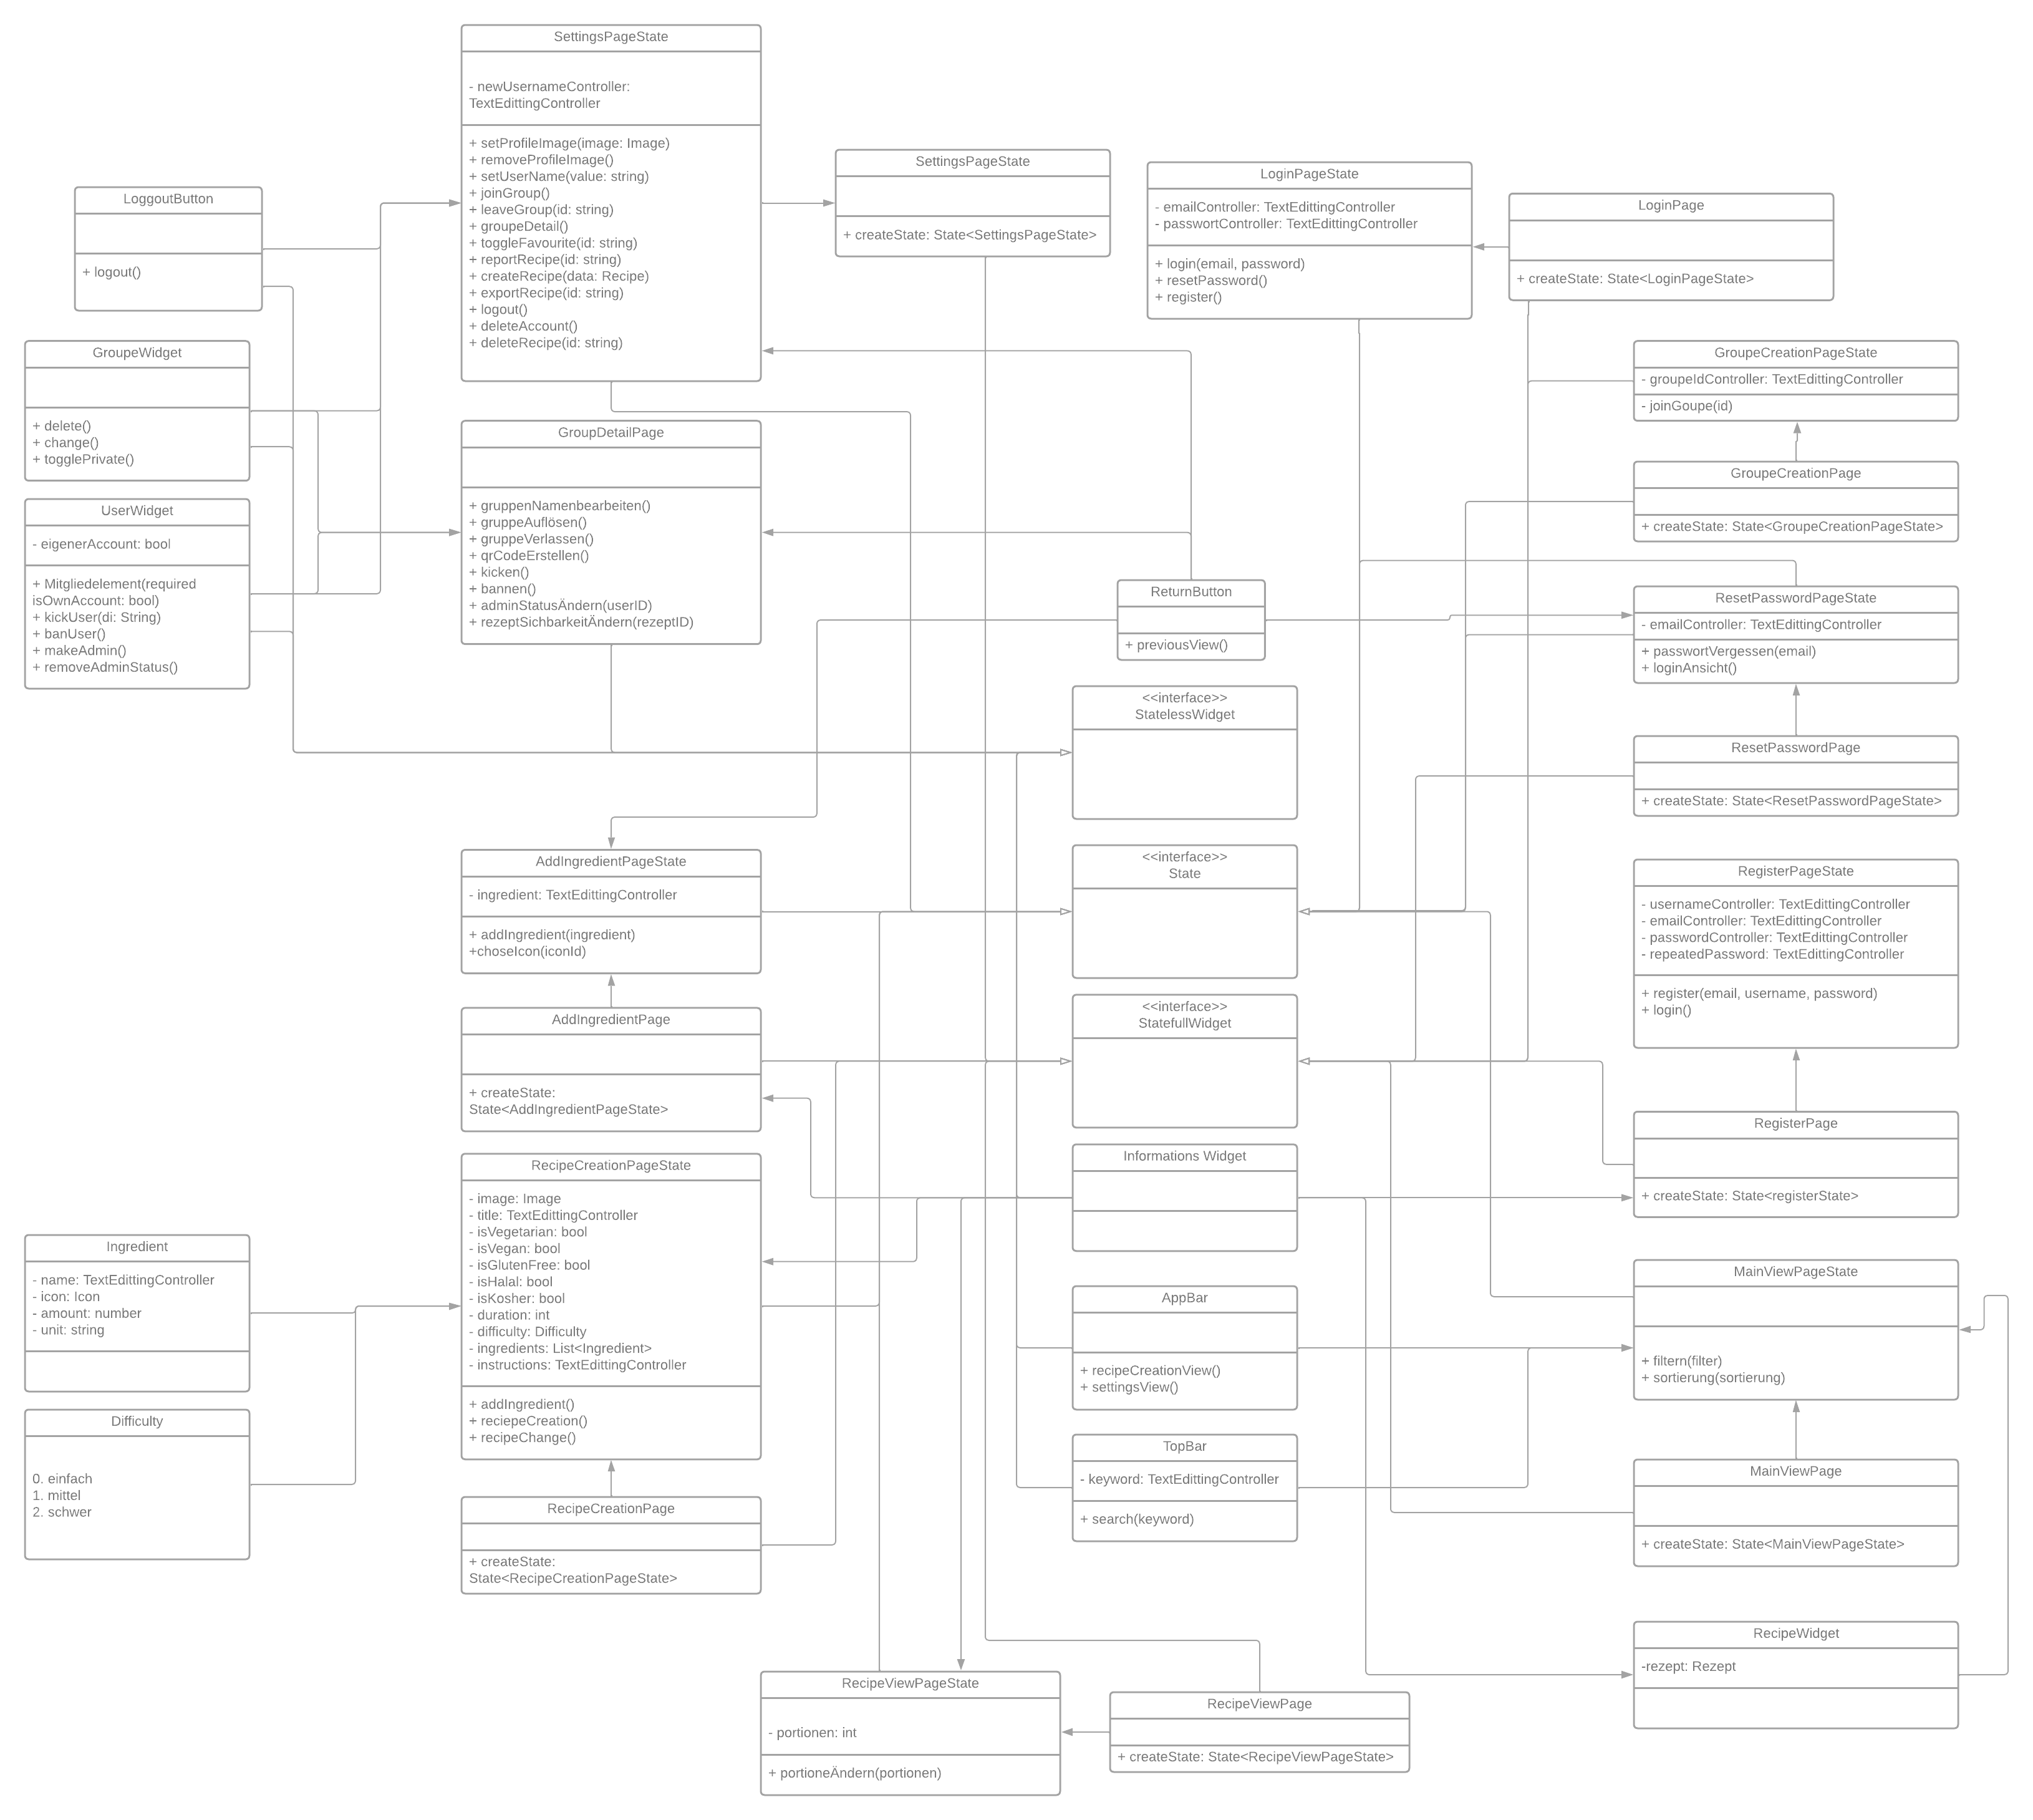
\includegraphics[width = \textwidth]{images/presentationLayer/presentationLayer.png}
    \caption{Klassendiagramm des Presentation Layer}
    \label{fig:presentation-layer}
\end{figure}

\newpage

\subsection{Hauptansicht}
Die Klassen beinhalten alle nötigen Funktionen und Attribute, um die Hauptansicht darzustellen.

\subsubsection{MainViewPage}\label{sec:MainViewPage}
\subsubsection*{Methode}
\paragraph*{createState: State<MainViewPageState>} Der Konstruktor für den MainViewPageState.

\subsubsection{MainViewPageState}\label{sec:MainViewPageState}
\subsubsection*{Methode}

\paragraph*{filtering(filter: FilteringMethods)} Alle Rezepte werden dem Filterkriterium gefiltert.
\paragraph*{sorting(sort: SortingMethods)} Alle Rezepte werden nach dem Sortierkriterium sortiert.

\subsubsection{TopBar}\label{sec:TopBar}
\subsubsection*{Attribute}
\paragraph*{keyword: TextEdittingController} Durch den Nutzer eingegebene Zeichenkette für die Suche.

\subsubsection*{Methode}
\paragraph*{ search(keyword: TextEdittingController)} Durchsucht alle Rezepte und gibt die aus, deren Rezepttitel zu dem Schlagwort passen.


\subsubsection{AppBar} \label{sec:AppBar}
\subsubsection*{Attribute}
\paragraph*{mainView: Boolean} Der Boolean gibt an ob das AppBar Element in Hauptansicht verwendet wird.
\paragraph*{recipeCreationView: Boolean} Der Boolean gibt an ob das AppBar Element in Rezept-Erstellungs-Ansicht verwendet wird.
\paragraph*{settingsView: Boolean} Der Boolean gibt an ob das AppBar Element in Einstellungsansicht verwendet wird.

\subsubsection*{Methode}
\paragraph*{AppBar(required mainView: Boolean ,required recipeCreationView: Boolean ,required settingsView: Boolean )} Der Konstruktor für den AppBar. Alle Parameter müssen angegeben werden.
\paragraph*{mainView()} Die Hauptansicht wird aufgerufen.
\paragraph*{recipeCreationView()} Die Rezept-Erstellungs-Ansicht wird aufgerufen.
\paragraph*{settingsView()} Die Einstellungsansicht wird aufgerufen.


\subsubsection{InformationElement}\label{sec:InformationElement}
\subsubsection*{Attribute}
\paragraph*{information: InformationCategories} Gibt an, welche Information in dem Widget dargestellt werden soll.
\paragraph*{text: string} Der Text, der in dem Widget angezeigt werden kann.

\subsubsection*{Methode}
\paragraph*{InformationWidget(required information: InformationCategories , text: string)} Konstruktor für Information Element. Eine Information Kategorie muss angegeben werden.


\subsubsection{SortingMethods}\label{sec:SortingMethods}
Ein Enum, der alle Sortierungsmethoden beinhält.
\subsubsection*{Content}
\paragraph*{alphabetical} Die Rezepte werden alphabetisch sortiert.
\paragraph*{difficulty} Die Rezepte werden nach dem \glslink{schwierigkeit}{Schwierigkeitsgrad} sortiert.
\paragraph*{date} Die Rezepte werden nach dem Hinzufügedatum sortiert.

\subsubsection{FilteringMethods}\label{sec:FilteringMethods}
Ein Enum, der alle Filter Methoden beinhält.
\subsubsection*{Content}
\paragraph*{favorites} Die Rezepte werden nach Favoriten gefiltert.
\paragraph*{difficultyEasy} Die Rezepte werden nach dem \glslink{schwierigkeit}{Schwierigkeitsgrad} einfach gefiltert.
\paragraph*{difficultyMedium} Die Rezepte werden nach dem \glslink{schwierigkeit}{Schwierigkeitsgrad} mittel gefiltert.
\paragraph*{difficultyHard} Die Rezepte werden nach dem \glslink{schwierigkeit}{Schwierigkeitsgrad} schwer gefiltert.
\paragraph*{labelVegetarian} Die Rezepte werden nach dem \gls{label} vegetarisch gefiltert.
\paragraph*{labelVegan} Die Rezepte werden nach dem \gls{label} vegan gefiltert.
\paragraph*{labelGlutenFree} Die Rezepte werden nach dem \gls{label} glutenfrei gefiltert.
\paragraph*{labelHalal} Die Rezepte werden nach dem \gls{label} halal gefiltert.
\paragraph*{labelKoscher} Die Rezepte werden nach dem \gls{label} koscher gefiltert.


\subsubsection{InformationCategories}\label{sec:InformationCategories}
Ein Enum der alle Information Kategorien beinhält.
\subsubsection*{Content}
\paragraph*{duration} Das Widget gibt die Zubereitungsdauer an.
\paragraph*{difficultyEasy} Das Widget gibt den \glslink{schwierigkeit}{Schwierigkeitsgrad} einfach an.
\paragraph*{difficultyMedium} Das Widget gibt den \glslink{schwierigkeit}{Schwierigkeitsgrad} mittel an.
\paragraph*{difficultyHard} Das Widget gibt den \glslink{schwierigkeit}{Schwierigkeitsgrad} schwer an.
\paragraph*{labelVegetarian} Das Widget gibt das \gls{label} vegetarisch an.
\paragraph*{labelVegan} Das Widget gibt das \gls{label} vegan an.
\paragraph*{labelGlutenFree} Das Widget gibt das \gls{label} glutenfrei an.
\paragraph*{labelHalal} Das Widget gibt das \gls{label} halal an.
\paragraph*{labelKoscher} Das Widget gibt das \gls{label} koscher an.

\subsubsection*{RecipeElement (\ref{sec:InformationElement})}

\begin{figure}[htp]
    \begin{minipage}
        [t]{0.49\textwidth}
        \centering
        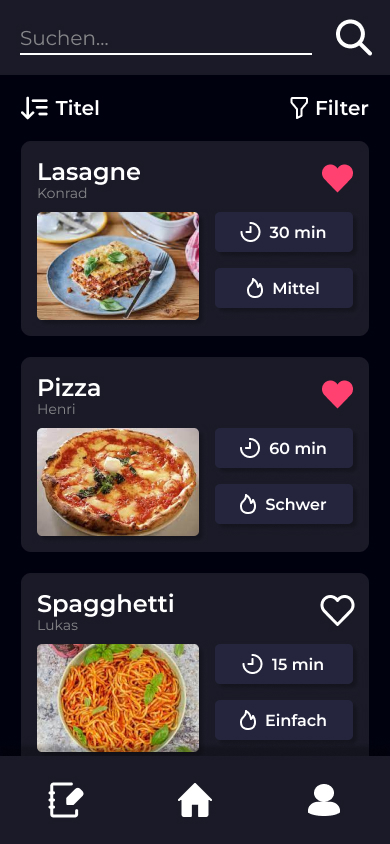
\includegraphics[height=80mm]{images/Presentation-layer/MainView.jpg}
        \caption{Hauptansicht}
    \end{minipage}
    \begin{minipage}
        [t]{0.49\textwidth}
        \centering
        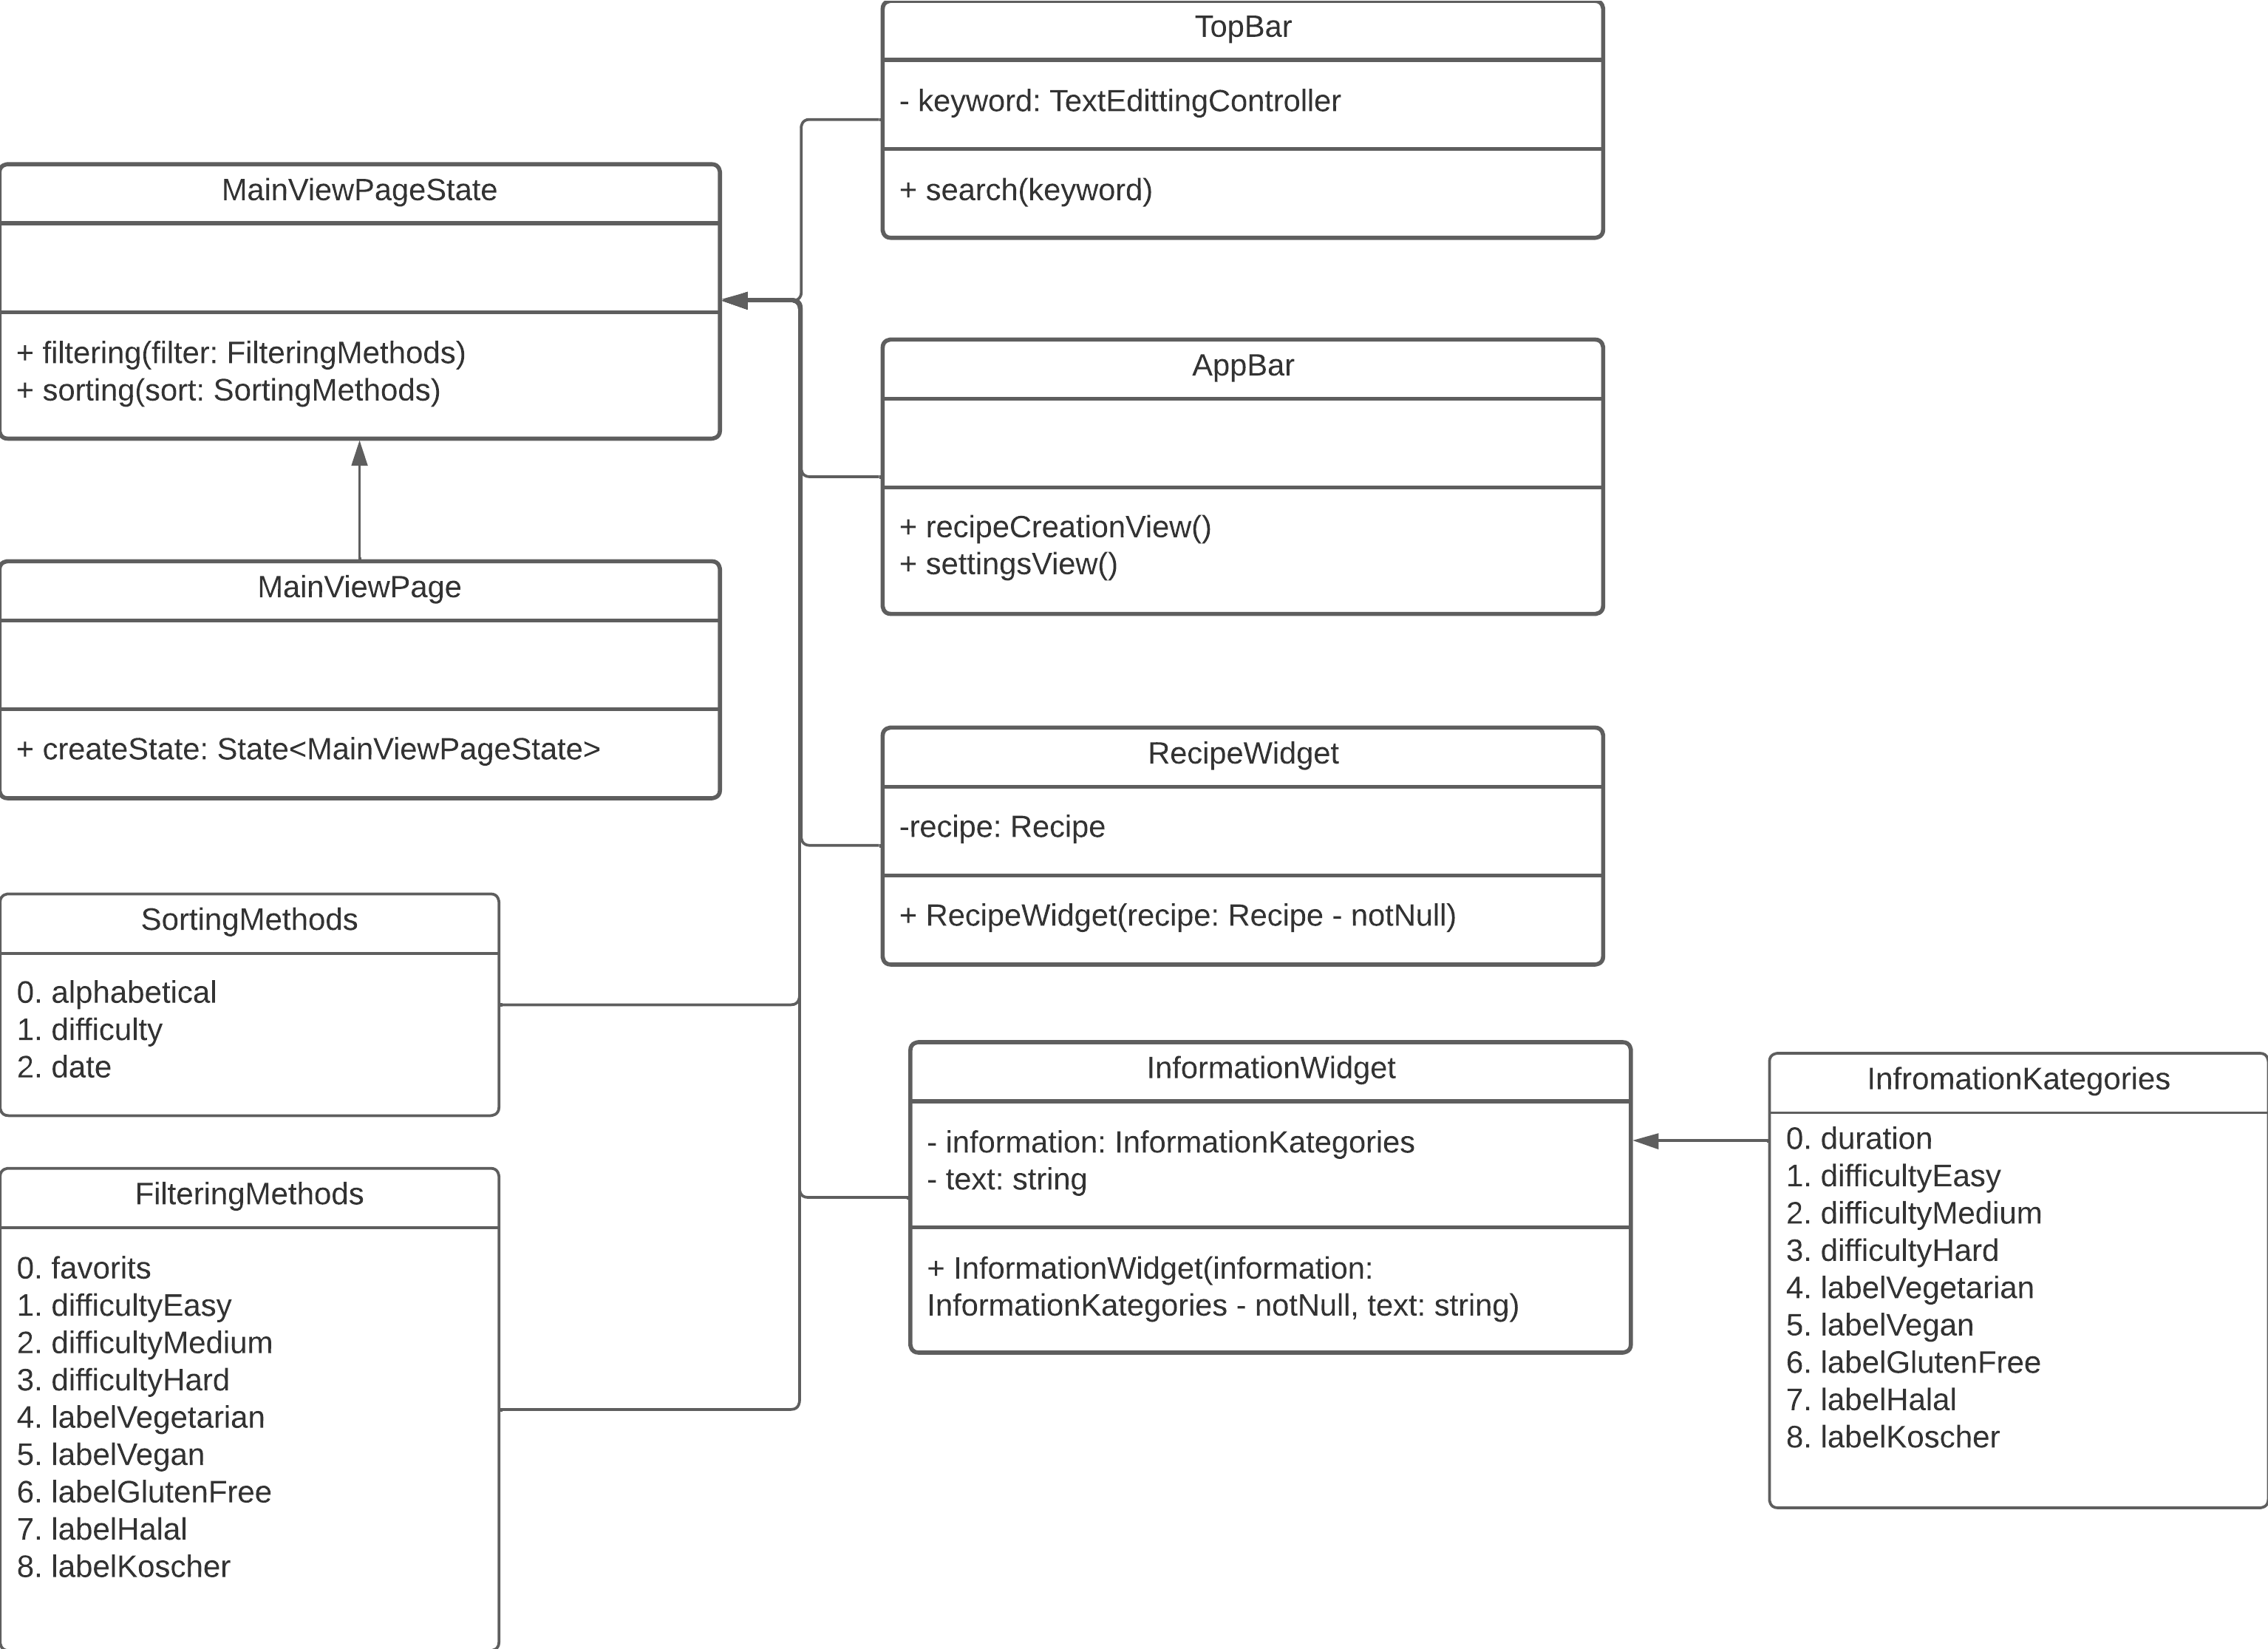
\includegraphics[width=0.95\textwidth]{images/Presentation-layer/MainViewClass.png}
        \caption{Klassen für Hauptansicht}
    \end{minipage}
\end{figure}

\subsection{Rezeptansicht}
Die Klassen beinhalten alle nötigen Funktionen und Attribute um die Hauptansicht darzustellen.

\subsubsection{RecipeViewPage}\label{sec:RecipeViewPage}
\subsubsection*{Methode}
\paragraph*{createState: State<RecipeViewPageState>} Konstruktor für den RecipeViewPageState.

\subsubsection{recipeViewPageState}\label{sec:RecipeViewPageState}
\subsubsection*{Attribute}
\paragraph*{portions: TextEdittingController} Eingegebene Ganzzahl für die die Zutatenmengen berechnet werden. Ist standardmäßig auf der Portionsgröße, die beim Rezepterstellen angegeben worden ist.

\subsubsection*{Methode}
\paragraph*{changePortions(portions: int)} Die neuen Mengenangaben für die Zutaten werden berechnet.

\subsubsection*{InformationElement (\ref{sec:InformationElement})}

\subsubsection{InformationCategories (\ref{sec:InformationCategories})}

\begin{figure}[htp]
    \begin{minipage}
        [t]{0.49\textwidth}
        \centering
        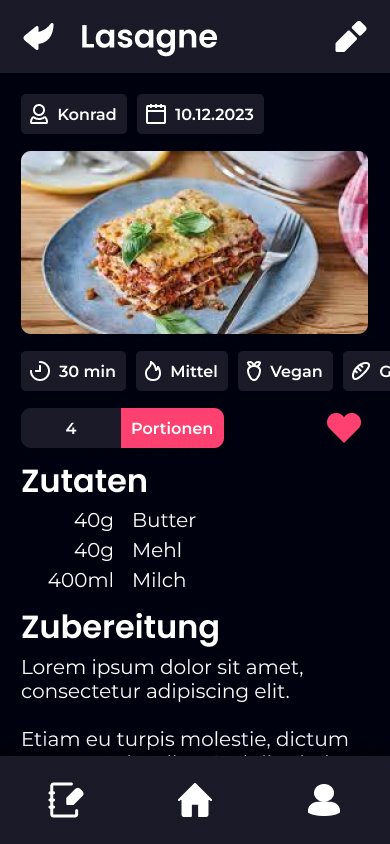
\includegraphics[height=80mm]{images/Presentation-layer/RecipeView.jpg}
        \caption{Rezeptansicht}
    \end{minipage}
    \begin{minipage}
        [t]{0.49\textwidth}
        \centering
        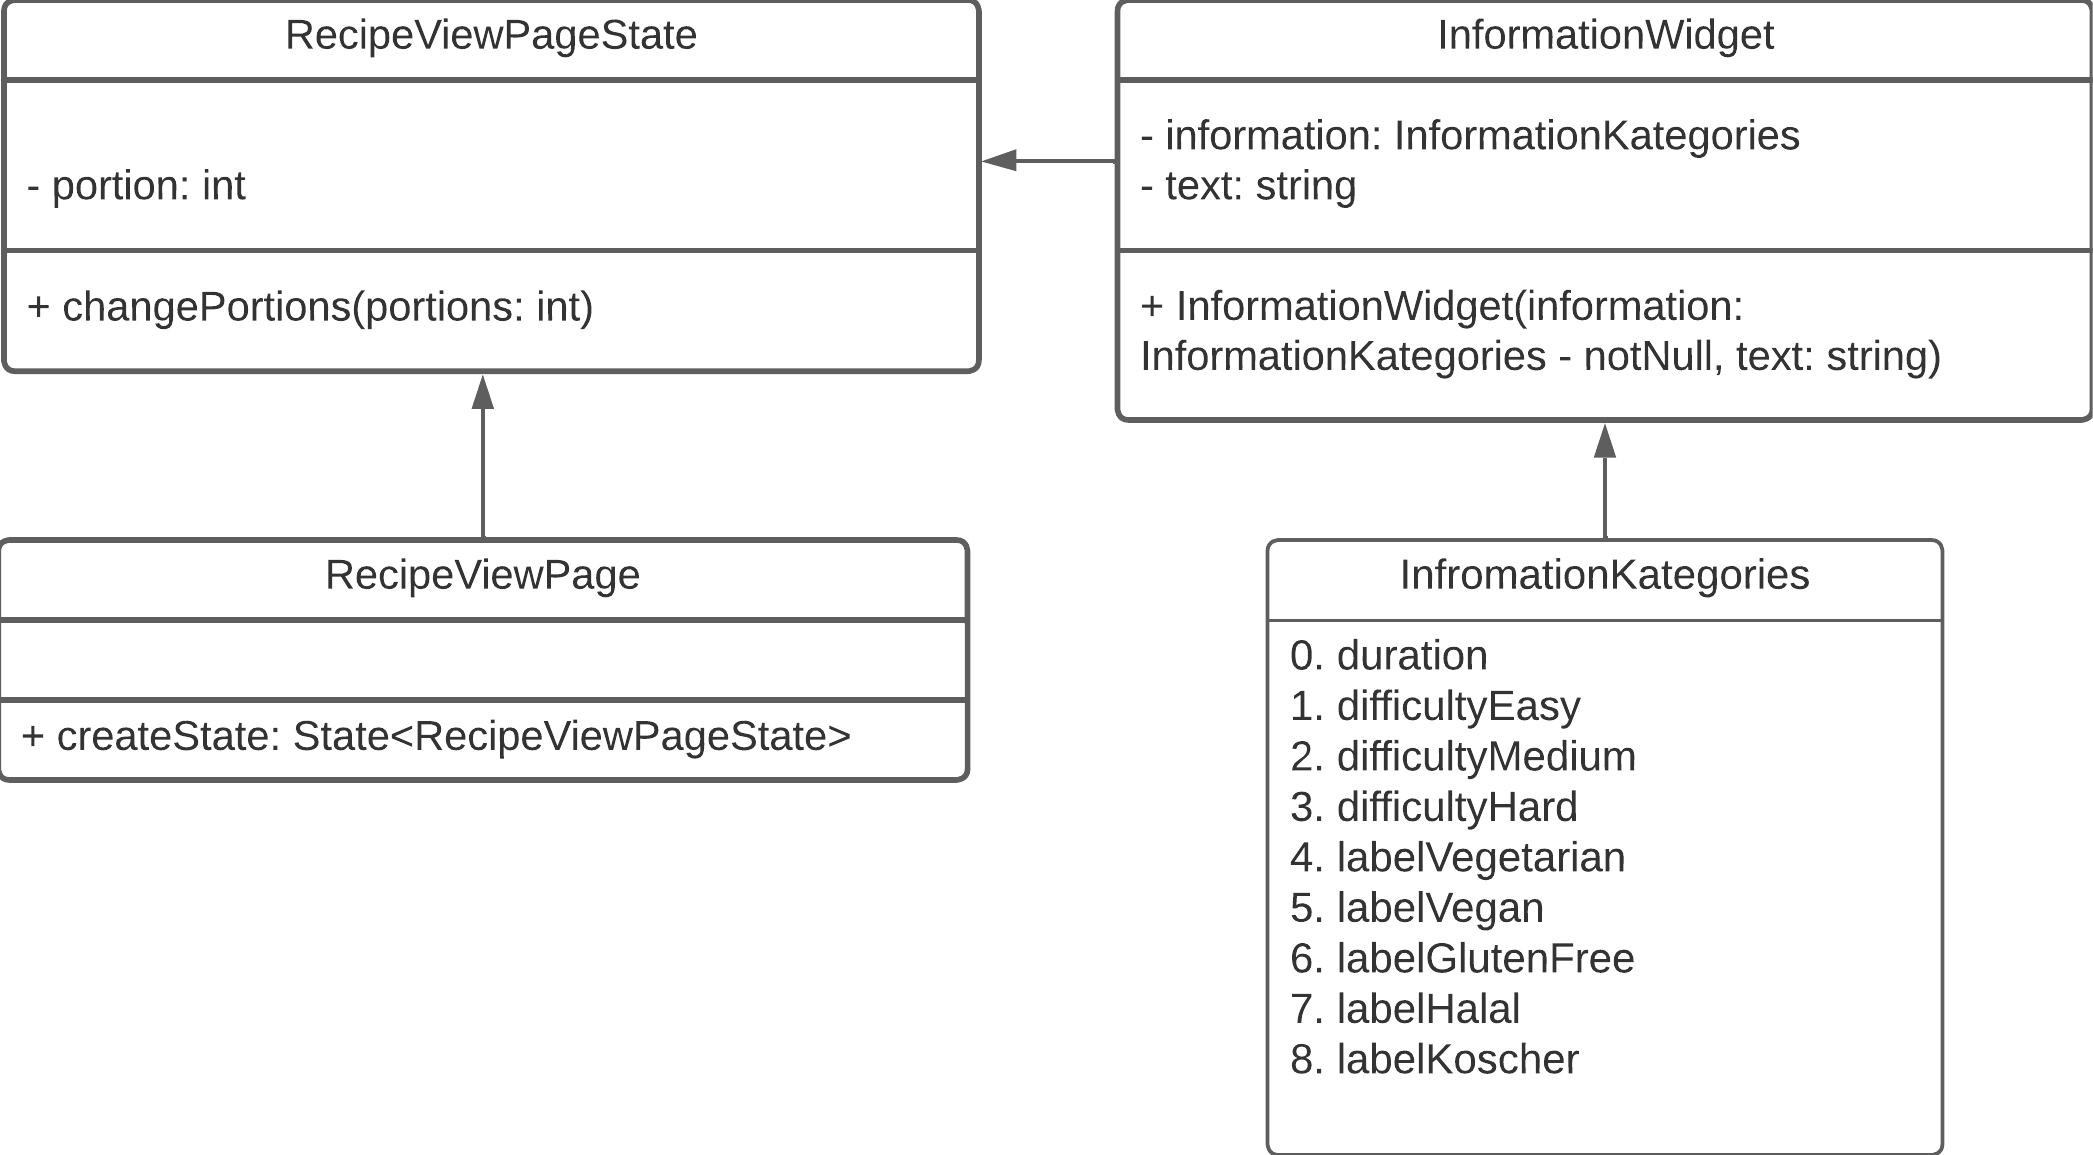
\includegraphics[width=0.95\textwidth]{images/Presentation-layer/RecipeViewClass.png}
        \caption{Klassen für Rezeptansicht}
    \end{minipage}
\end{figure}

\newpage

\subsection{Registrierungsansicht}
Die Klassen beinhalten alle nötigen Funktionen und Attribute um die Registrierungsansicht darzustellen.

\subsubsection{RegisterPage}\label{sec:RegisterPage}
\subsubsection*{Methode}
\paragraph*{createState: State<RegisterPageState>} Konstruktor für den RegisterPageState.

\subsubsection{RegisterPageState}\label{sec:RegisterPageState}
\subsubsection*{Attribute}
\paragraph*{usernameController: TextEdittingController} Die eingegebene Zeichenkette für den Benutzernamen des neuen Users.
\paragraph*{emailController: TextEdittingController} Die eingegebene Zeichenkette für die E-Mail-Adresse des neuen Users.
\paragraph*{passwordController: TextEdittingController} Die eingegebene Zeichenkette für das Passwort des neuen Accounts für den neuen User.
\paragraph*{repeatedPassword: TextEdittingController} Die eingegebene Zeichenkette für das wiederholte Passwort des neuen Accounts.

\subsubsection*{Methode}
\paragraph*{register(username: string, email: string, password: string, repeatedPassword: string)} Überprüft, ob das eingegeben Passwort mit dem wiederholten Passwort übereinstimmt und ruft dann die Funktion register() im UserRepository auf.
\paragraph*{login()} Die Loginansicht wird aufgerufen.

\subsubsection*{InformationElement (\ref{sec:InformationElement})}

\subsubsection{InformationCategories (\ref{sec:InformationCategories})}

\begin{figure}[htp]
    \begin{minipage}
        [t]{0.49\textwidth}
        \centering
        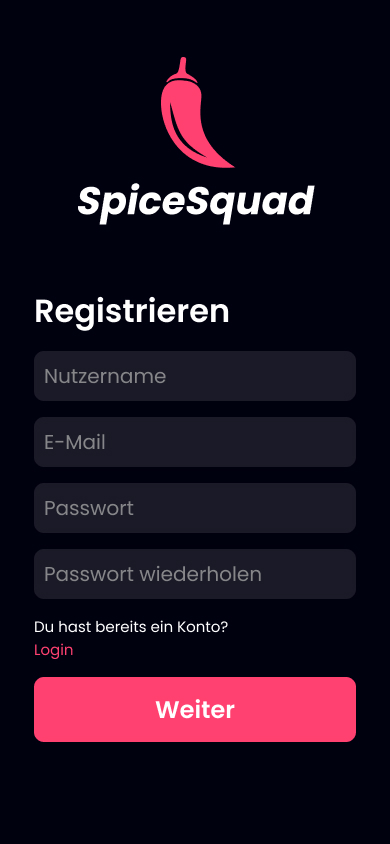
\includegraphics[height=80mm]{images/Presentation-layer/RegisterView.jpg}
        \caption{Registrierungsansicht}
    \end{minipage}
    \begin{minipage}
        [t]{0.49\textwidth}
        \centering
        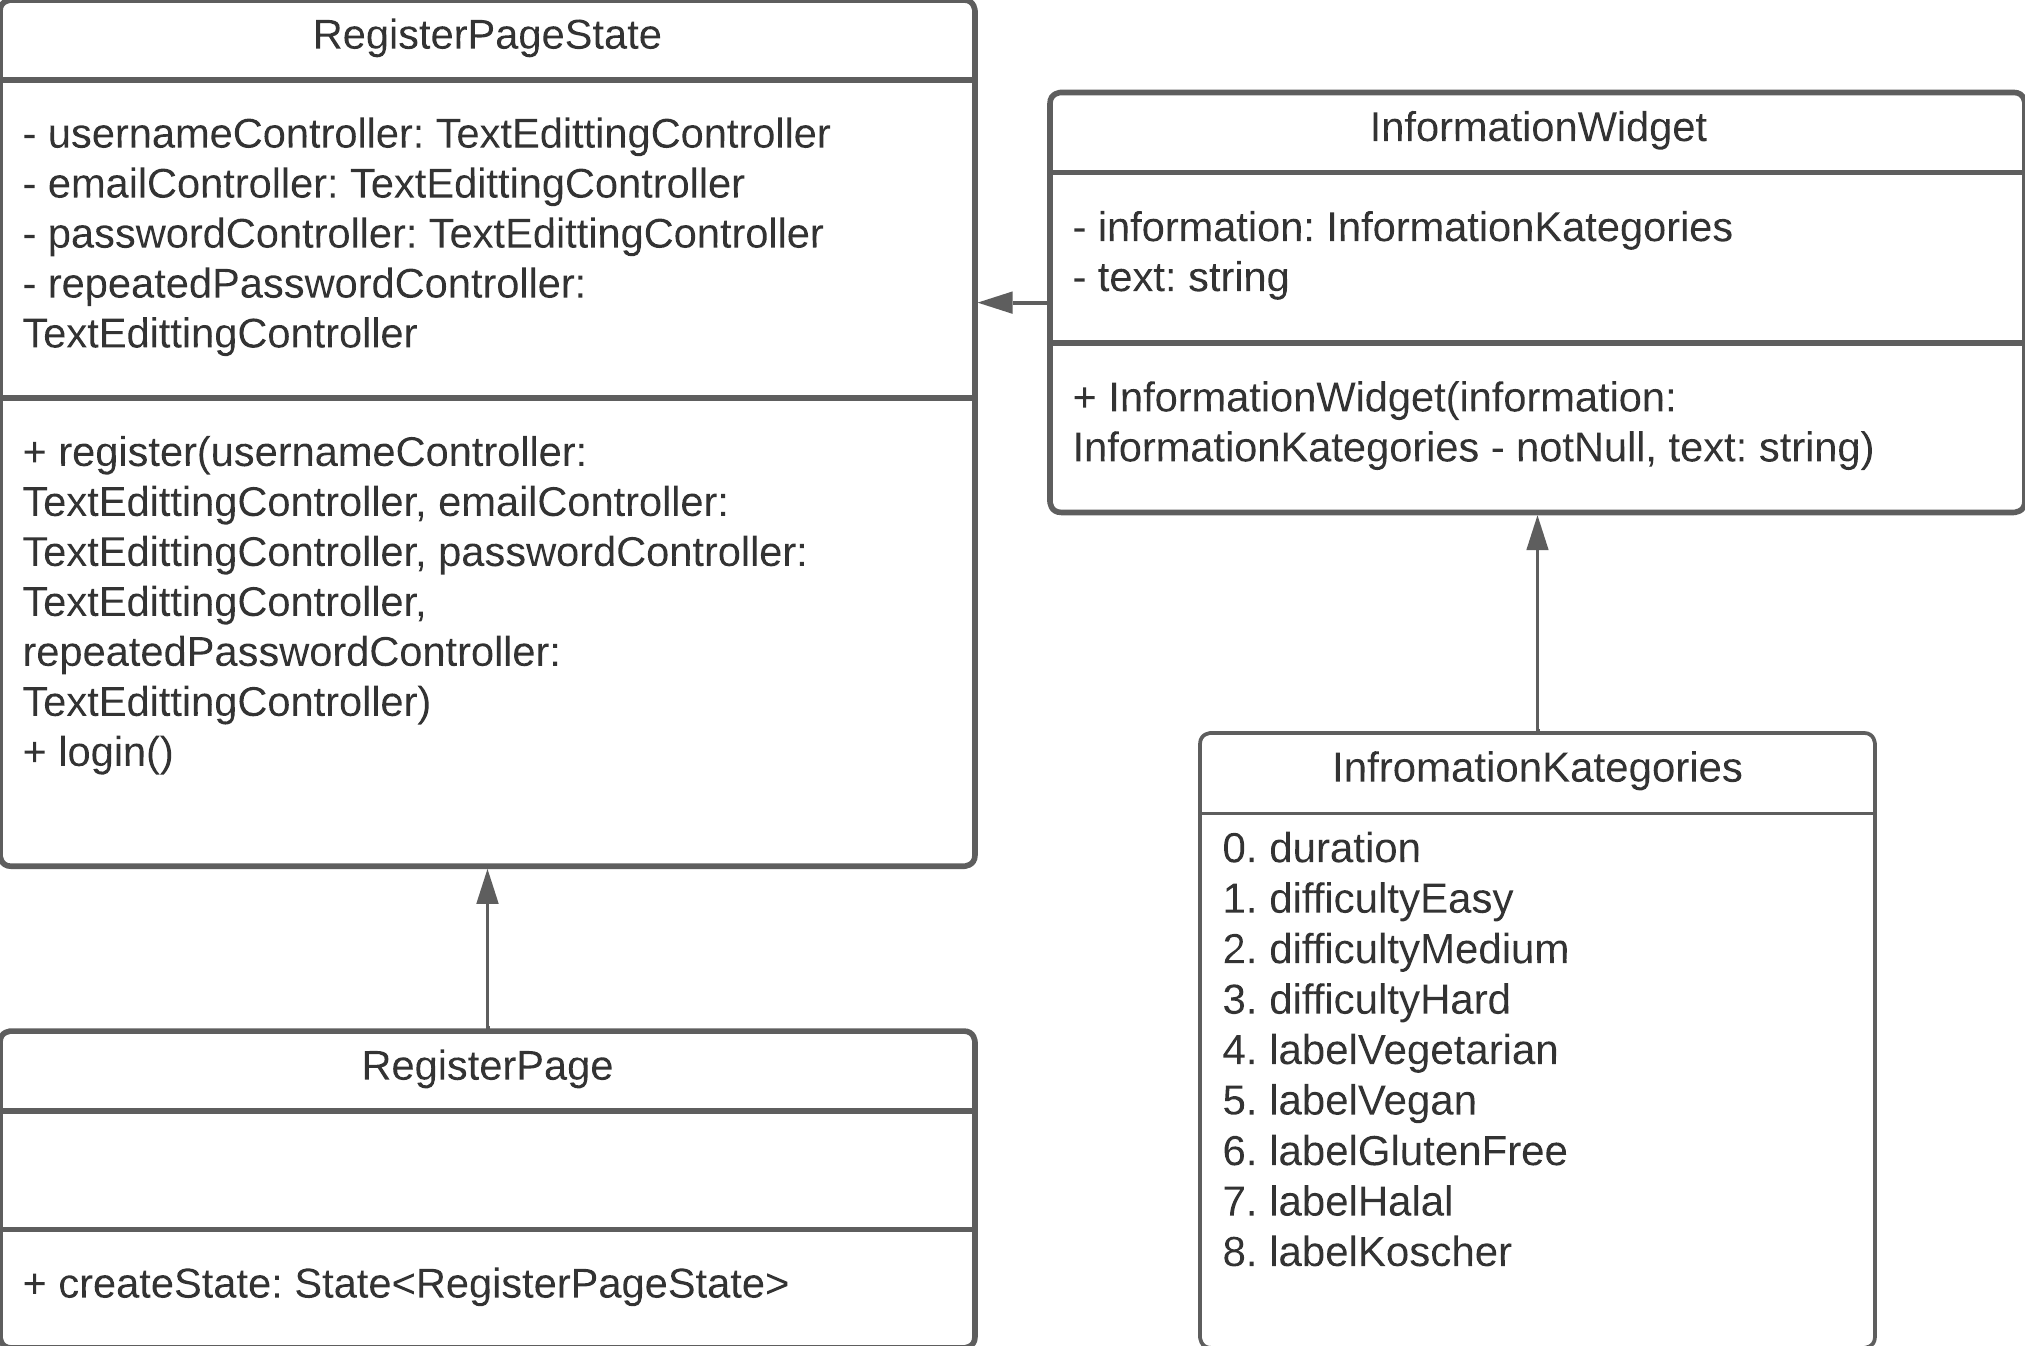
\includegraphics[width=0.95\textwidth]{images/Presentation-layer/RegisterViewClass.png}
        \caption{Klassen für Registrierungsansicht}
    \end{minipage}
\end{figure}

\newpage

\subsection{Passwort-Zurücksetzen-Ansicht}
Die Klassen beinhalten alle nötigen Funktionen und Attribute um die Passwort-Zurücksetzen-Ansicht darzustellen.

\subsubsection{ResetPasswordPage}\label{sec:ResetPasswordPage}
\subsubsection*{Methode}
\paragraph*{createState: State<ResetPasswordPageState>} Konstruktor für den ResetPasswordPageState.

\subsubsection{ResetPasswordPageState}\label{sec:ResetPasswordPageState}
\subsubsection*{Attribute}
\paragraph*{emailController: TextEdittingController} Die eingegebene Zeichenkette für die E-Mail-Adresse des Users.

\subsubsection*{Methode}
\paragraph*{resetPassword(email: string)} Überprüft die Korrektheit der E-Mail-Adresse und ruft die Funktionen resetPassword() im UserRepository auf.
\paragraph*{LoginView()} Die Loginansicht wird aufgerufen.

\subsubsection{ReturnButton}\label{sec:ReturnButton}
\subsubsection*{Methode}
\paragraph*{prevoiusView()} Die vorherige Ansicht wird aufgerufen. Es werden keine Daten gespeichert die in der Ansicht angegeben worden sind.

\begin{figure}[htp]
    \begin{minipage}
        [t]{0.49\textwidth}
        \centering
        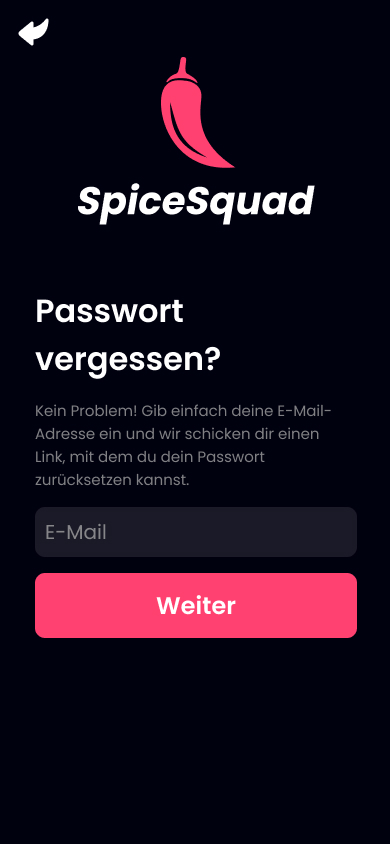
\includegraphics[height=80mm]{images/Presentation-layer/PasswordResetView.jpg}
        \caption{Passwort-Zurücksetzen-Ansicht}
    \end{minipage}
    \begin{minipage}
        [t]{0.49\textwidth}
        \centering
        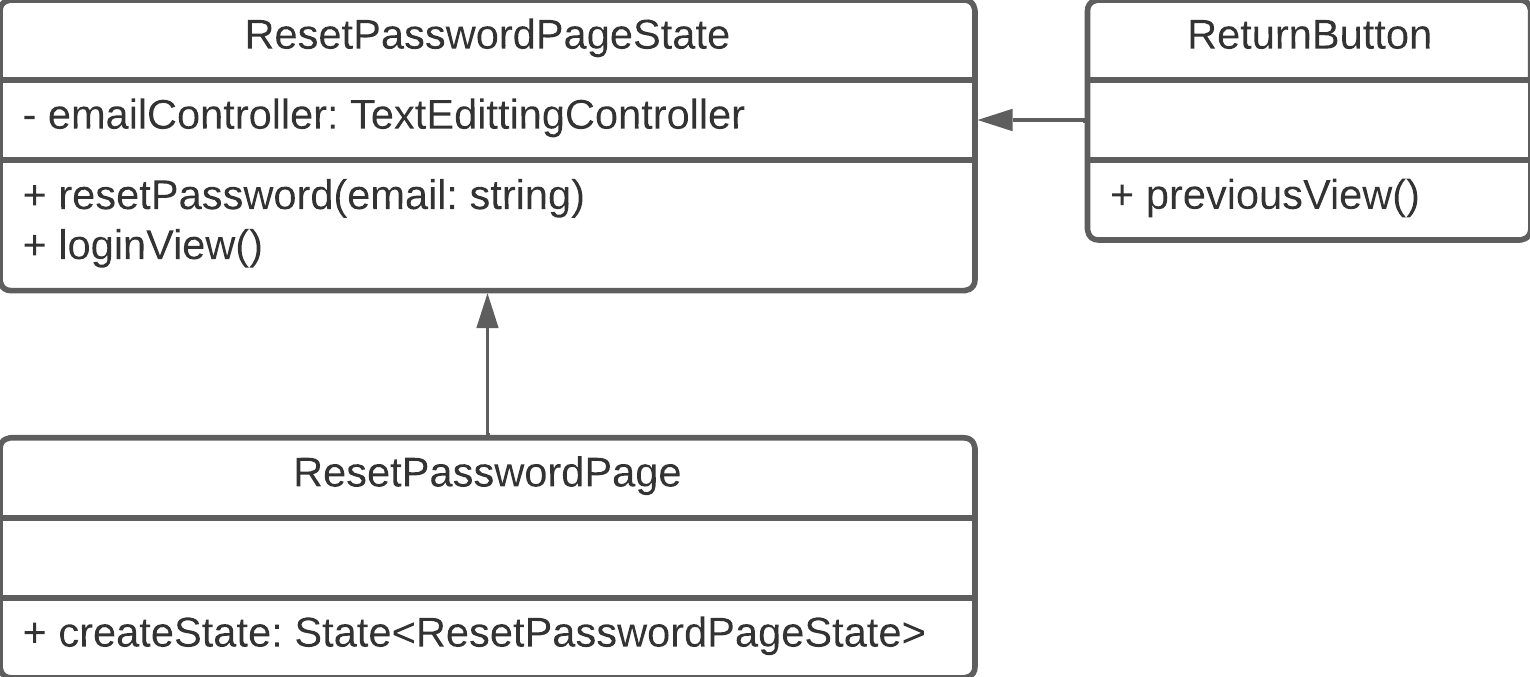
\includegraphics[width=0.95\textwidth]{images/Presentation-layer/PasswordResetViewClass.png}
        \caption{Klassen für Passwort-Zurücksetzen-Ansicht}
    \end{minipage}
\end{figure}

\newpage

\subsection{Anmeldungsansicht}
Die Klassen beinhalten alle nötigen Funktionen und Attribute, um die Anmeldungsansicht darzustellen.

\subsubsection{LoginPagePage}\label{sec:LoginPagePage}
\subsubsection*{Methode}
\paragraph*{createState: State<LoginPageState>} Konstruktor für den LoginPageState.

\subsubsection{LoginPageState}\label{sec:LoginPageState}
\subsubsection*{Attribute}
\paragraph*{emailController: TextEdittingController} Die eingegebene Zeichenkette für die E-Mail-Adresse des Users.
\paragraph*{passwortController: TextEdittingController} Die eingegebene Zeichenkette für das Passwort des Users.

\subsubsection*{Methode}
\paragraph*{login(email: string, password: string)} Überprüft die Eingaben und ruft die Funktionen createGroup() im UserRepository auf.
\paragraph*{resetPasswordView()}  Die Passwort-Zurücksetzen-Ansicht wird aufgerufen.
\paragraph*{registerView()}  Die Registrierungsansicht wird aufgerufen.

\begin{figure}[htp]
    \begin{minipage}
        [t]{0.49\textwidth}
        \centering
        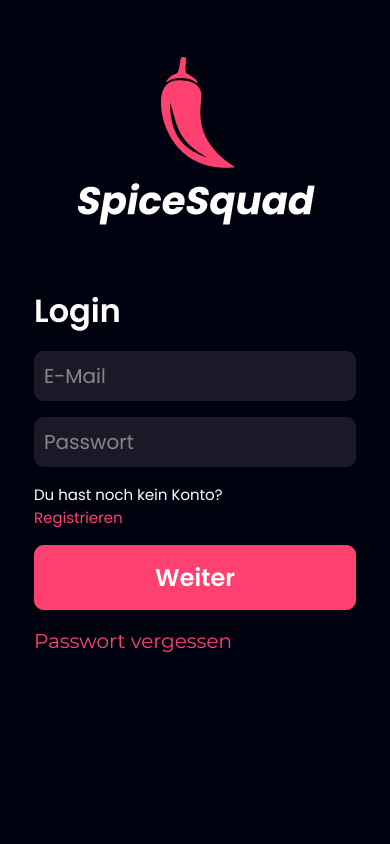
\includegraphics[height=80mm]{images/Presentation-layer/LoginView.jpg}
        \caption{Anmeldungsansicht}
    \end{minipage}
    \begin{minipage}
        [t]{0.49\textwidth}
        \centering
        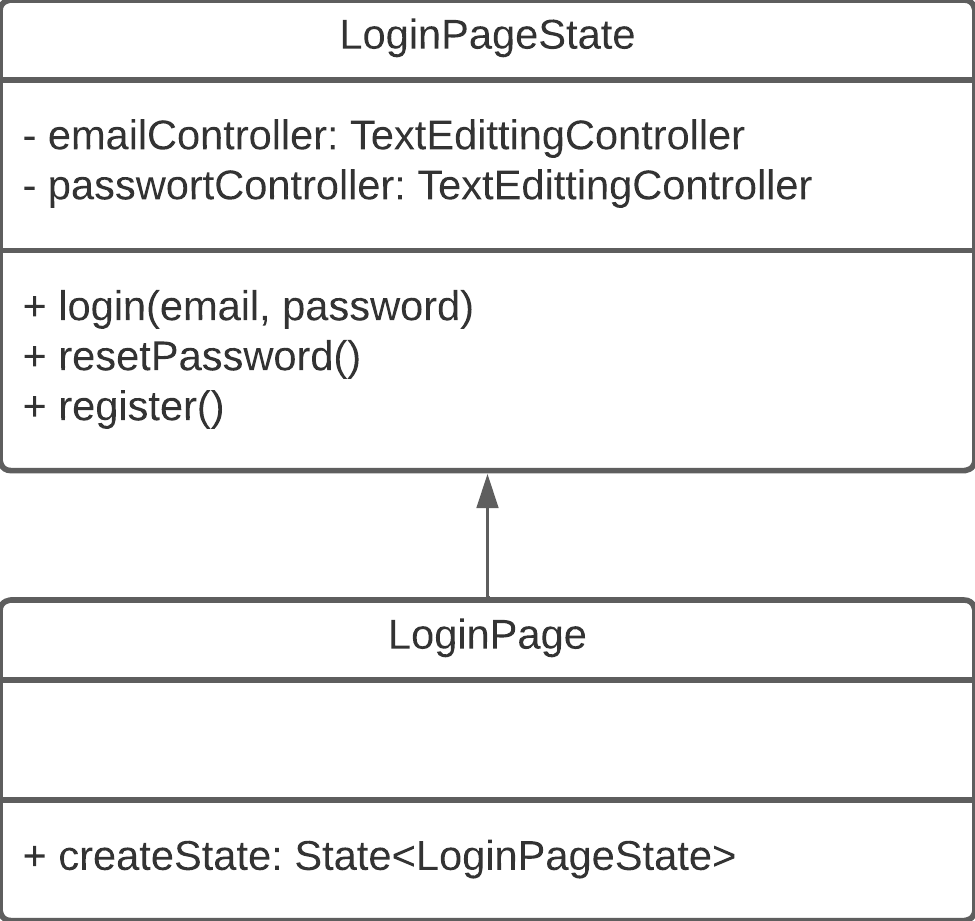
\includegraphics[width=0.95\textwidth]{images/Presentation-layer/LoginViewClass.png}
        \caption{Klassen für Anmeldungsansicht}
    \end{minipage}
\end{figure}

\newpage

\subsection{Gruppen-Erstellungs-Ansicht}
Die Klassen beinhalten alle nötigen Funktionen und Attribute um die Gruppen-Erstellungs-Ansicht darzustellen.

\subsubsection{GroupCreationPage}\label{sec:GroupCreationPage}
\subsubsection*{Methode}
\paragraph*{createState: State<GroupCreationPageState>} Konstruktor für den GroupCreationPageState.

\subsubsection{GroupCreationPageState}\label{sec:GroupCreationPageState}
\subsubsection*{Attribute}
\paragraph*{GroupNameController: TextEdittingController} Die eingegebene Zeichenkette für den Namen der neuen Gruppe.

\subsubsection*{Methode}
\paragraph*{createGroupe(name: string)} Überprüft den Gruppenname und ruft die Funktionen createGroupe() im GroupeService auf.
\paragraph*{joinGroupeView()}  Die Gruppen-Beitritts-Ansicht wird aufgerufen.
\paragraph*{mainView()} Die Hauptansicht wird aufgerufen.


\paragraph*{createGroup(name: string)} Überprüft den Gruppennamen und ruft die Funktionen createGroup() im GroupService auf.
\paragraph*{joinGroupView()}  Die Gruppen-Beitritts-Ansicht wird aufgerufen.

\begin{figure}[htp]
    \begin{minipage}
        [t]{0.49\textwidth}
        \centering
        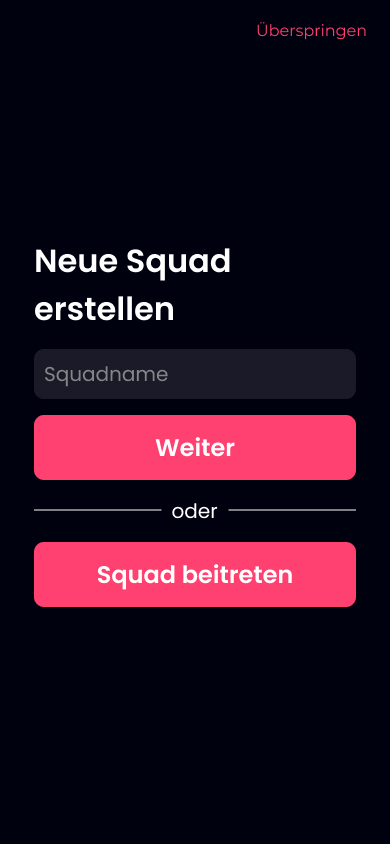
\includegraphics[height=80mm]{images/Presentation-layer/GroupCreationView.jpg}
        \caption{Gruppen-Erstellungs-Ansicht}
    \end{minipage}
    \begin{minipage}
        [t]{0.49\textwidth}
        \centering
        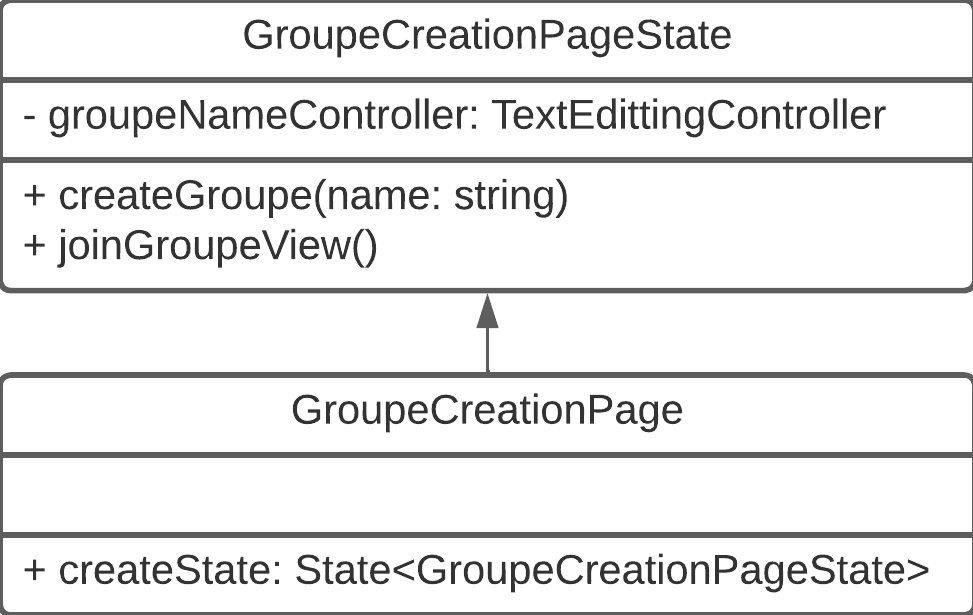
\includegraphics[width=0.95\textwidth]{images/Presentation-layer/GroupCreationViewClass.png}
        \caption{Klassen für Gruppen-Erstellungs-Ansicht}
    \end{minipage}
\end{figure}

\newpage

\subsection{Gruppen-Beitritts-Ansicht}
Die Klassen beinhalten alle nötigen Funktionen und Attribute um die Gruppen-Beitritts-Ansicht darzustellen.

\subsubsection{GroupJoiningPage}\label{sec:GroupJoiningPage}
\subsubsection*{Methode}
\paragraph*{createState: State<GroupJoiningPageState>} Der Konstruktor für den GroupJoiningPageState.

\subsubsection{GroupJoiningPageState}\label{sec:GroupJoiningPageState}
\subsubsection*{Attribute}
\paragraph*{groupeNameController: TextEdittingController} Die eingegebene Zeichenkette für den Namen der beizutreten Gruppe.

\subsubsection*{Methode}
\paragraph*{joinGroup()} Überprüft den Gruppenname und ruft die Funktionen joinGroupe() im GroupeService auf.
\paragraph*{joinGroupQr()} Das CameraElement wird aufgerufen.
\paragraph*{createGroupeView()}  Die Gruppen-Beitritts-Ansicht wird aufgerufen.
\paragraph*{mainView()} Die Hauptansicht wird aufgerufen.

\subsubsection*{CameraElement}\label{sec:CameraElement}
\subsubsection*{Attribute}
\paragraph*{barcodes: List<Barcode>}  Der gescannte QR-Code.

\begin{figure}[htp]
    \begin{minipage}
        [t]{0.49\textwidth}
        \centering
        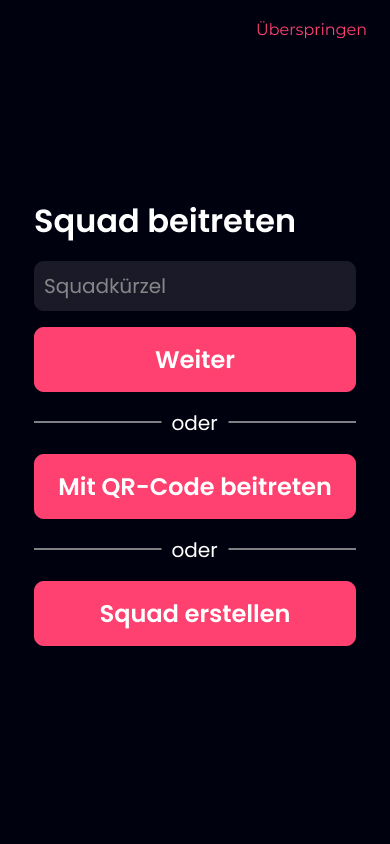
\includegraphics[height=80mm]{images/Presentation-layer/GroupJoiningView.jpg}
        \caption{Gruppen-Beitritts-Ansicht}
    \end{minipage}
    \begin{minipage}
        [t]{0.49\textwidth}
        \centering
        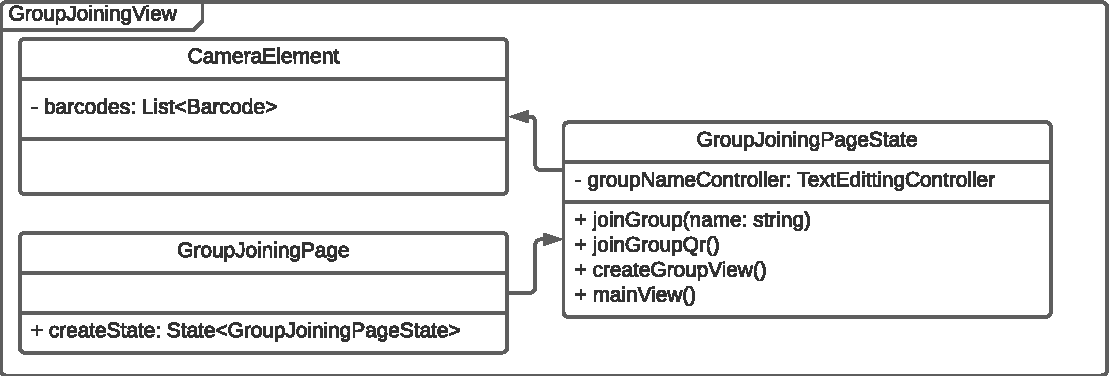
\includegraphics[width=0.95\textwidth]{images/Presentation-layer/GroupJoiningViewClass.pdf}
        \caption{Klassen für Gruppen-Beitritts-Ansicht}
    \end{minipage}
\end{figure}

\newpage

\subsection{Gruppen-Detail-Ansicht}
Die Klassen beinhalten alle nötigen Funktionen und Attribute um die Gruppen-Detail-Ansicht darzustellen.

\subsubsection{GroupDetailPage}\label{sec:GroupDetailPage}
\subsubsection*{Attribute}
\paragraph*{group: Group} Die Gruppe, deren Details dargestellt werden.
\paragraph*{newTitle: TextEdittingController} Die eingegebe Zeichenkette für den neuen Gruppennamen.

\subsubsection*{Methode}
\paragraph*{GroupDetailPage(required group: Group)} Ein Konstruktor für eine GroupDetailPage. Der Parameter muss angegeben werden.
\paragraph*{setGroupTitle(newTitle: string)} Die Eingabe wird Überprüft und die Funktion setGroupName() im GroupeService wird aufgerufen.
\paragraph*{deleteGroup()} Das ConfirmationElement wird aufgerufen und bei positiver Rückmeldung wird die Funktion kickUser() im GroupeService wird aufgerufen. Bei negativer Rückmeldung ändert sich nichts.
\paragraph*{leaveGroup()} Das ConfirmationElement wird aufgerufen und bei positiver Rückmeldung wird die Funktion leaveGroup() im GroupeService wird aufgerufen. Bei negativer Rückmeldung ändert sich nichts.

\paragraph*{getQRCode()} Die QR-Code-Ansicht wird aufgerufen.
\paragraph*{getGroupTitel()} Der Gruppentitel wird in der Zwischenablage gespeichert.

\subsubsection{ConfirmationElement} \label{sec:ConfirmationElement}
\subsubsection*{Attribute}
\paragraph*{text: string} Der Text, der im Widget angezeigt werden soll.

\subsubsection*{Methode}
\paragraph*{ConfirmationElement(required text: string)} Ein Konstruktor für ein ConfirmationElement, wobei ein Text angegeben werden muss.
\paragraph*{decline()} Dem Erzeugter wird true zurückgegeben.
\paragraph*{accept()} Dem Erzeugter wird false zurückgegeben.


\subsubsection{OptionElement}\label{sec:OptionElement}
\subsubsection*{Attribute}
\paragraph*{user: User} Der darzustellende User.

\subsubsection*{Methode}
\paragraph*{OptionElement(required user: User)} Ein Konstruktor für ein OptionElement. Der Parameter muss angegeben werden.
\paragraph*{kickUser()} Das ConfirmationElement wird aufgerufen und bei positiver Rückmeldung wird die Funktion kickUser() im UserSettingsService wird aufgerufen. Bei negativer Rückmeldung ändert sich nichts.
\paragraph*{banUser()} Das ConfirmationElement wird aufgerufen und bei positiver Rückmeldung wird die Funktion banUser() im UserSettingsService wird aufgerufen. Bei negativer Rückmeldung ändert sich nichts.
\paragraph*{makeAdmin()} Das ConfirmationElement wird aufgerufen und bei positiver Rückmeldung wird die Funktion makeAdmin() im UserSettingsService wird aufgerufen. Bei negativer Rückmeldung ändert sich nichts.
\paragraph*{removeAdminStatus()} Das ConfirmationElement wird aufgerufen und bei positiver Rückmeldung wird die Funktion removeAdminStatus() im UserSettingsService wird aufgerufen. Bei negativer Rückmeldung ändert sich nichts.


\subsubsection{RecipeElement}\label{sec:RecipeElement}
\subsubsection*{Attribute}
\paragraph*{recipe: Recipe} Das darzustellende Rezept.
\paragraph*{view: Boolean} Ein Boolean der angibt, ob die Sichtbarkeit des Rezepts verändert werden darf oder nicht.
\paragraph*{settingsView: Boolean} Ein Boolean der angibt, ob das Widget in der Einstellungsansicht verwendet wird.

\subsubsection*{Methode}
\paragraph*{RecipeElement(required recipe: Recipe,required view: boolean,required settingsView: boolean)} Ein Konstruktor für ein RecipeElement. Alle Parameter müssen angegeben werden.
\paragraph*{togglePrivate()} Die Sichtbarkeit des Rezepts für die Gruppe ausgeblendet werden soll, wenn settingsView false ist. Wenn settingsView auf true steht wird das Rezept für alle Gruppen ausgeblendet.
\paragraph*{delete()} Das ConfirmationElement wird aufgerufen und bei positiver Rückmeldung wird die Funktion deleteRecipe() im RecipeService aufgerufen. Bei negativer Rückmeldung ändert sich nichts.
\paragraph*{export()} Die Funktion exportRecipe() im RecipeService wird aufgerufen.

\subsubsection{UserElement}\label{sec:UserElement}
\subsubsection*{Attribute}

\paragraph*{user: User} Der darzustellende User.
\paragraph*{isOwnAccount: Boolean} Ein Boolean der Angibt ob es sich um den eigenen Account handelt.

\subsubsection*{Methode}
\paragraph*{UserElement(required user: User,required isOwnAccount: bool)} Ein Konstruktor für ein UserElement. Alle Parameter müssen angegeben werden.
\paragraph*{options()} Das OptionElement wird aufgerufen.

\subsubsection*{ReturnButton (\ref{sec:ReturnButton})}

\subsubsection*{ConfirmationElement (\ref{sec:ConfirmationElement})}

\begin{figure}[htp]
    \begin{minipage}
        [t]{0.49\textwidth}
        \centering
        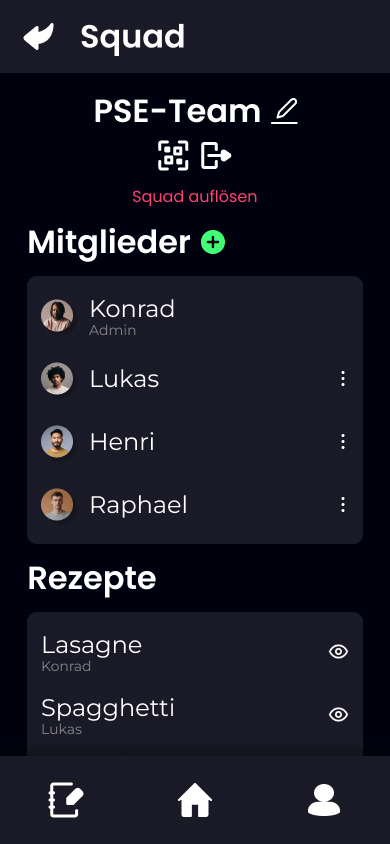
\includegraphics[height=80mm]{images/Presentation-layer/GroupDetailView.jpg}
        \caption{Gruppen-Detail-Ansicht}
    \end{minipage}
    \begin{minipage}
        [t]{0.49\textwidth}
        \centering
        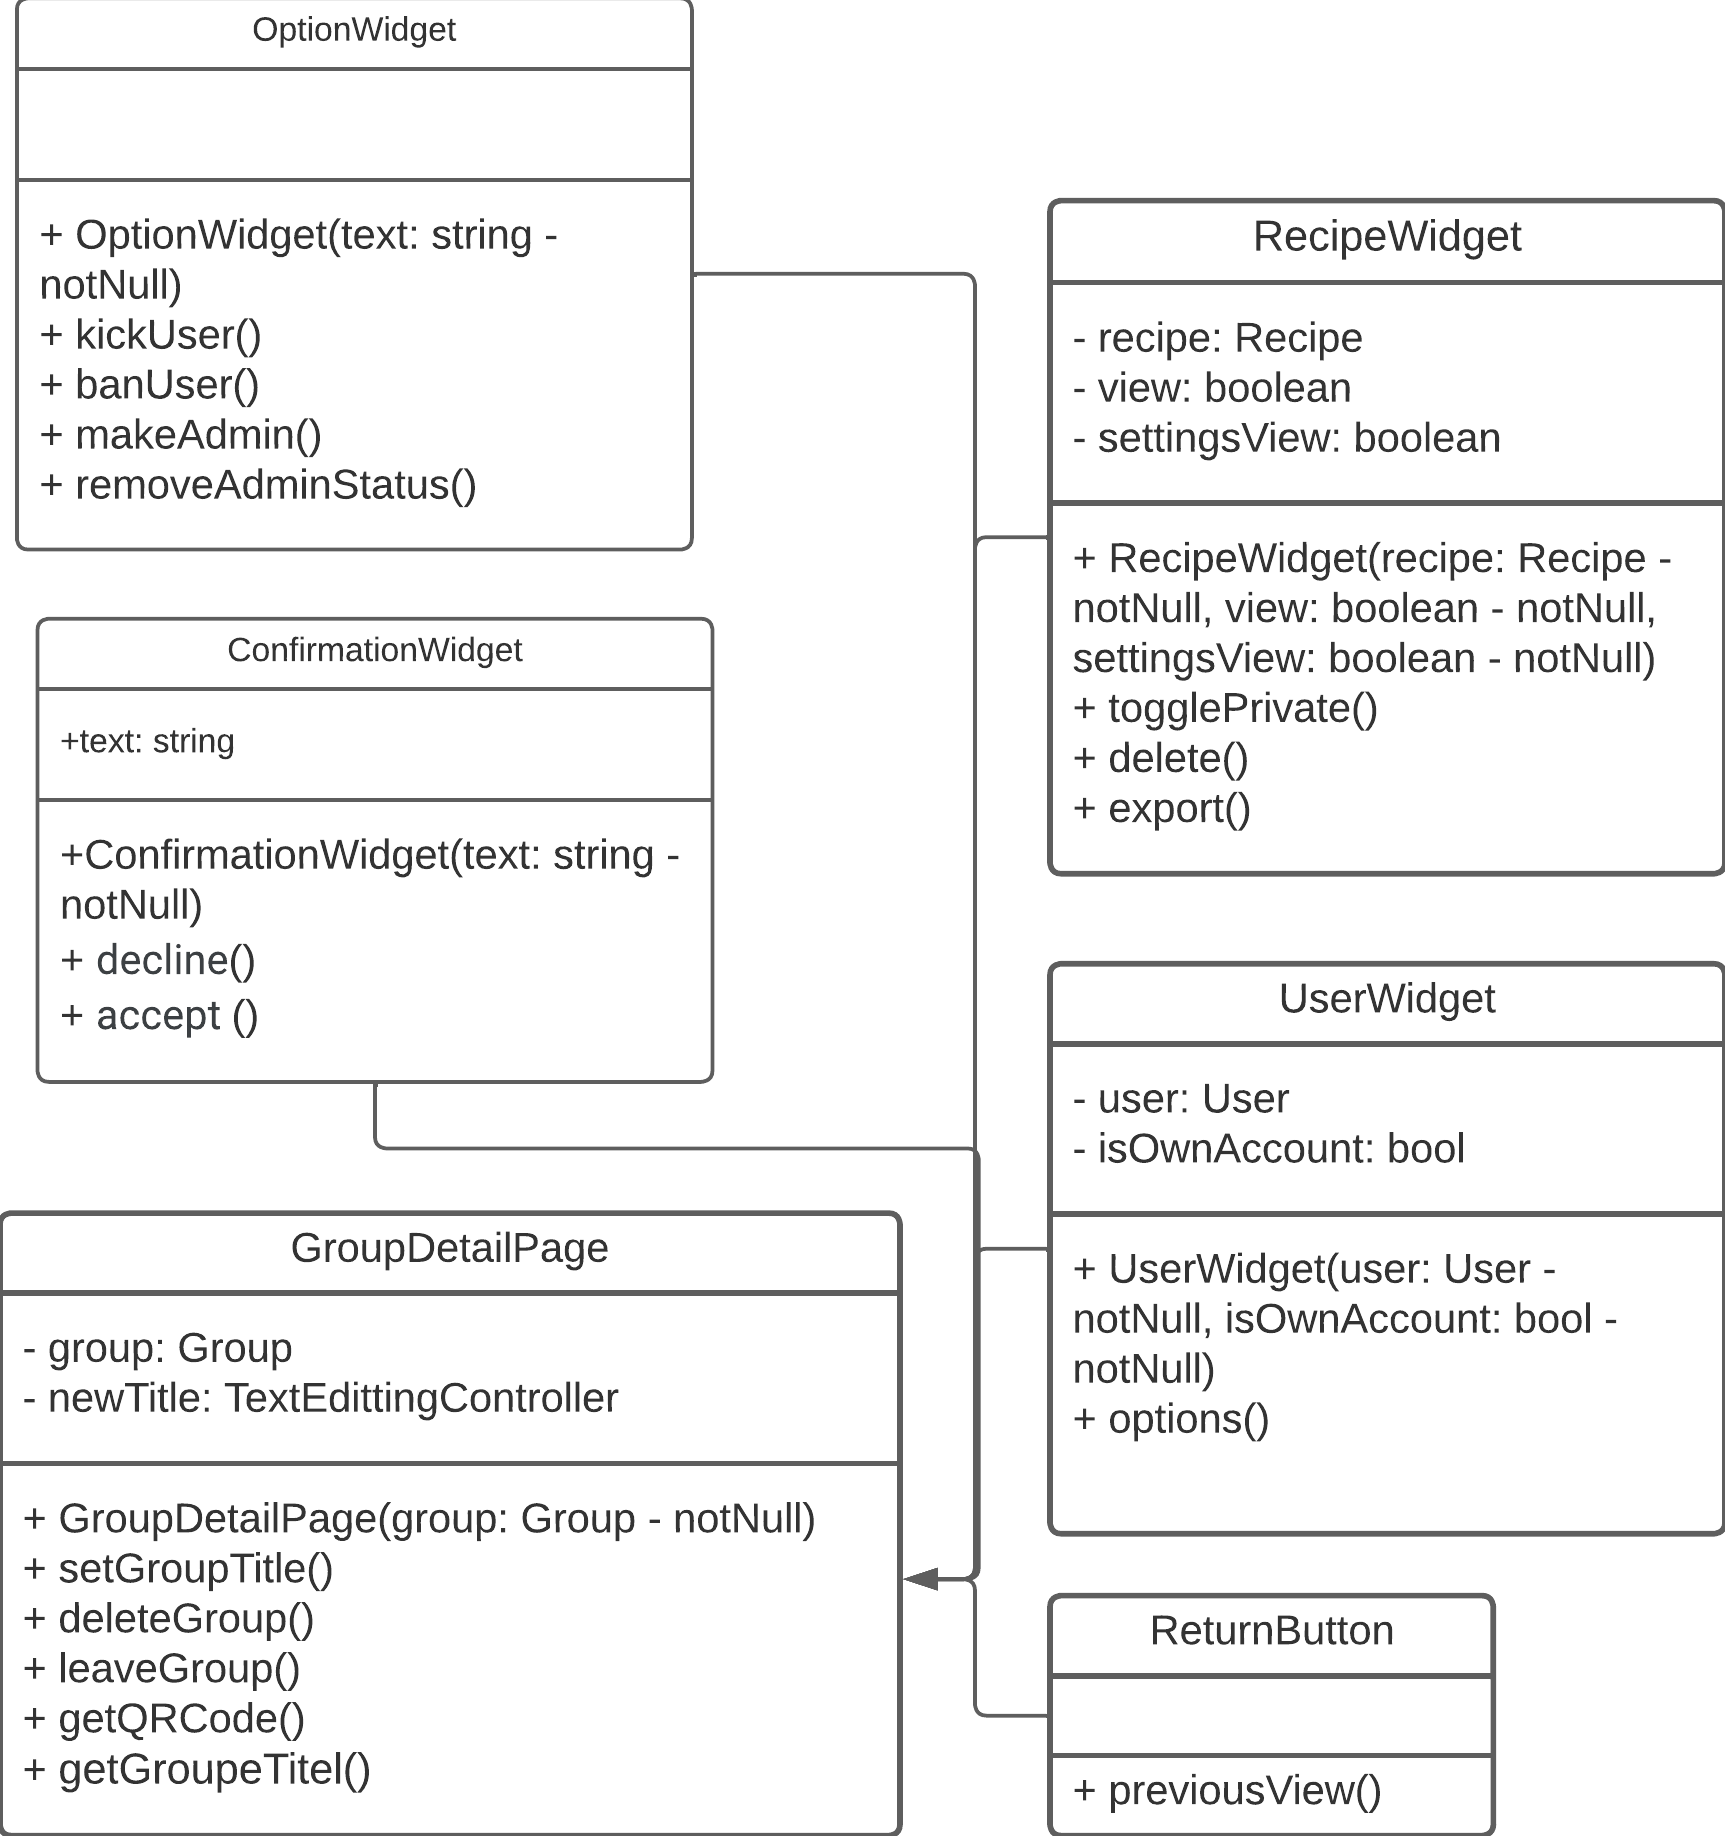
\includegraphics[width=0.95\textwidth]{images/Presentation-layer/GroupDetailViewClass.png}
        \caption{Klassen für Gruppen-Detail-Ansicht}
    \end{minipage}
\end{figure}

\newpage

\subsection{Rezept-Erstellungs-Ansicht}
Die Klassen beinhalten alle nötigen Funktionen und Attribute um die Rezept-Erstell-Ansicht darzustellen.

\subsubsection{RecipeCreationPage}\label{sec:RecipeCreationPage}
\subsubsection*{Methode}
\paragraph*{createState: State<RecipeCreationPageState>} Konstruktor für den RecipeCreationPageState.

\subsubsection{RecipeCreationPageState}\label{sec:RecipeCreationPageState}
\subsubsection*{Attribute}
\paragraph*{image: blob} Hochgeladenes Bild, welches den anderen Nutzern in der Rezeptansicht angezeigt werden soll.
\paragraph*{title: TextEdittingController (notNull)} Die eingegebene Zeichenkette für den Titel des Rezepts. Die Zeichenkette kann maximal 64 Zeichen lang sein und muss ausgefüllt sein.
\paragraph*{is\_Vegetarian: Boolean} Der vom Nutzer angegebene Boolean, ob das \gls{label} Vegetarisch dem Leser angezeigt werden soll. Ist standartmäßig auf false.
\paragraph*{is\_Vegan: Boolean} Der vom Nutzer angegebene Boolean, ob das \gls{label} Vegan dem Leser angezeigt werden soll. Ist standartmäßig auf false.
\paragraph*{is\_GlutenFree: Boolean} Der vom Nutzer angegebene Boolean, ob das \gls{label} Glutenfrei dem Leser angezeigt werden soll.  Ist standartmäßig auf false.
\paragraph*{is\_Halal: Boolean} Der vom Nutzer angegebene Boolean, ob das \gls{label} Halal dem Leser angezeigt werden soll.  Ist standartmäßig auf false.
\paragraph*{is\_Kosher: Boolean} Der vom Nutzer angegebene Boolean, ob das \gls{label} Koscher dem Leser angezeigt werden soll.  Ist standartmäßig auf false.
\paragraph*{duration: TextEdittingController (notNull)} Die vom Nutzer eingegebene Ganzzahl, welche die Zubereitungszeit in Minuten angibt. Muss angegeben werden.
\paragraph*{difficulty: Difficulty (notNull)} Die vom Nutzer ausgewählte \gls{schwierigkeit} des Rezepts. Muss angegeben werden.
\paragraph*{ingredients: Ingredients[]} Eine Liste an Ingerdients, welche in der AddIngredientPage erstellt wurde.
\paragraph*{instructions: TextEdittingController (notNull)} Die vom Nutzer angegeben Zeichenkette für die Beschreibung des Rezepts. Muss angegeben werden.

\subsubsection*{Methode}
\paragraph*{addIngredient()} Die Page AddIngredientPage wird aufgerufen.
\paragraph*{recipeSave()} Die Methode ruft, abhängig davon ob das Rezept neu erstellt wird oder nur verändert wurde, entweder recipeCreation() oder recipeChange() auf.

\subsubsection{Difficulty}\label{sec:Difficulty}
Ein Enum der alle \glslink{schwierigkeit}{Schwierigkeitsgrade} beinhält.
\subsubsection*{Content}
\paragraph*{easy} Der \glslink{schwierigkeit}{Schwierigkeitsgrad} einfach.
\paragraph*{medium} Der \glslink{schwierigkeit}{Schwierigkeitsgrad} mittel.
\paragraph*{hard} Der \glslink{schwierigkeit}{Schwierigkeitsgrad} schwer.

\subsubsection*{IngredientElement}\label{sec:IngredientElement}
Die Klasse beschreibt eine Widget dass eine Zutat darstellt.
\subsubsection*{Attribute}
\paragraph*{ingredient: Ingredient} Die darzustellende Zutat.

\subsubsection*{Methode}
\paragraph*{delete()} Das IngredientElement wird nicht mehr in der Rezept-Erstellungs-Ansicht angezeigt und ist die Zutat ist nicht mehr teil des Rezepts.

\subsubsection*{InformationElement (\ref{sec:InformationElement})}

\subsubsection*{InformationKategories}

\subsubsection*{ReturnButton (\ref{sec:ReturnButton})}

\subsubsection*{AppBar (\ref{sec:AppBar})}
\begin{figure}[htp]
    \begin{minipage}
        [t]{0.49\textwidth}
        \centering
        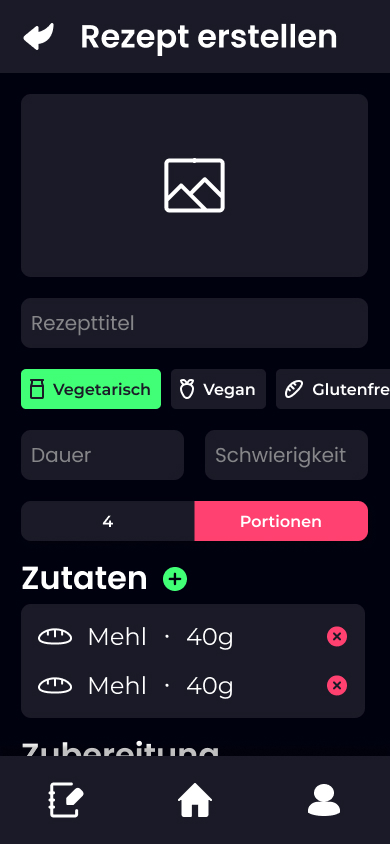
\includegraphics[height=80mm]{images/Presentation-layer/RecipeCreationView.jpg}
        \caption{Rezept-Erstellungs-Ansicht}
    \end{minipage}
    \begin{minipage}
        [t]{0.49\textwidth}
        \centering
        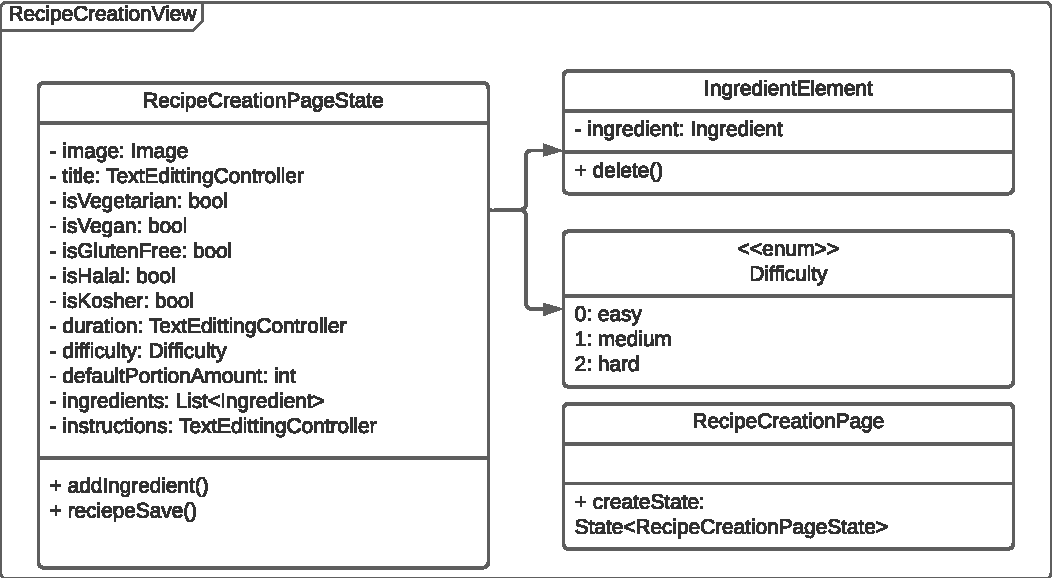
\includegraphics[width=0.95\textwidth]{images/Presentation-layer/RecipeCreationViewClass.pdf}
        \caption{Klassen für Rezept-Erstellungs-Ansicht}
    \end{minipage}
\end{figure}

\newpage

\subsection{Zutaten-Auswahl-Ansicht}
Die Klassen beinhalten alle nötigen Funktionen und Attribute um die Zutaten-Auswahl-Ansicht darzustellen.

\subsubsection{AddIngredientPage}\label{sec:AddIngredientPage}
\subsubsection*{Methode}
\paragraph*{createState: State<AddIngredientPageState>} Der Konstruktor für den AddIngredientPageState.

\subsubsection{AddIngredientPageState}\label{sec:AddIngredientPageState}
\subsubsection*{Attribute}
\paragraph*{ingredientController: TextEdittingController} Die eingegebene Zeichenkette für den Namen der neunen Zutat.

\subsubsection*{Methode}
\paragraph*{searchIngredient(input: string)} Überprüft die Eingabe und ruft die Funktion getAllIngredientNames() im IngredientService auf.
\paragraph*{addIngredient(ingredient: Ingredient)}  Erstellt aus den Eingaben ein Objekt der Klasse Ingredient und kehrt zurück zur Rezept-Erstellungs-Ansicht.

\subsubsection*{Ingredient}\label{sec:Ingredient}
\subsubsection*{Attribute}
\paragraph*{name: string} Der Name der Zutat.
\paragraph*{iconId: string} Die Id des Icons, welche zu der Zutat ausgewählt worden ist.
\paragraph*{amount: int} Die Mengenangabe für die Zutat.
\paragraph*{unit: string} Die Einheit der Mengenangabe.

\subsubsection*{ChoseIconElement}\label{sec:ChoseIconElement}
\subsubsection*{Methode}
\paragraph*{choseIcon(iconId: String)} Speichert das ausgewählte Icon mit der Zutat ab.

\paragraph*{IconElement}\label{sec:IconElement}
\subsubsection*{Attribute}
\paragraph*{iconId: String} Die Id des Icons, welches dargestellt werden soll.

\subsubsection*{ReturnButton (\ref{sec:ReturnButton})}


\begin{figure}[htp]
    \begin{minipage}
        [t]{0.49\textwidth}
        \centering
        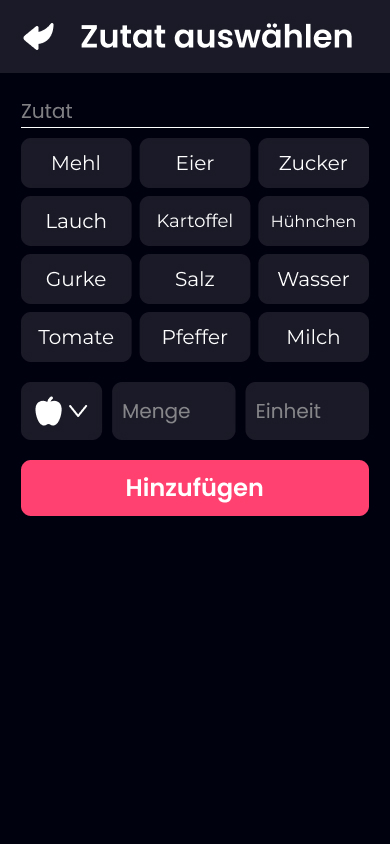
\includegraphics[height=80mm]{images/Presentation-layer/IngredientPickerView.jpg}
        \caption{Zutaten-Auswahl-Ansicht}
    \end{minipage}
    \begin{minipage}
        [t]{0.49\textwidth}
        \centering
        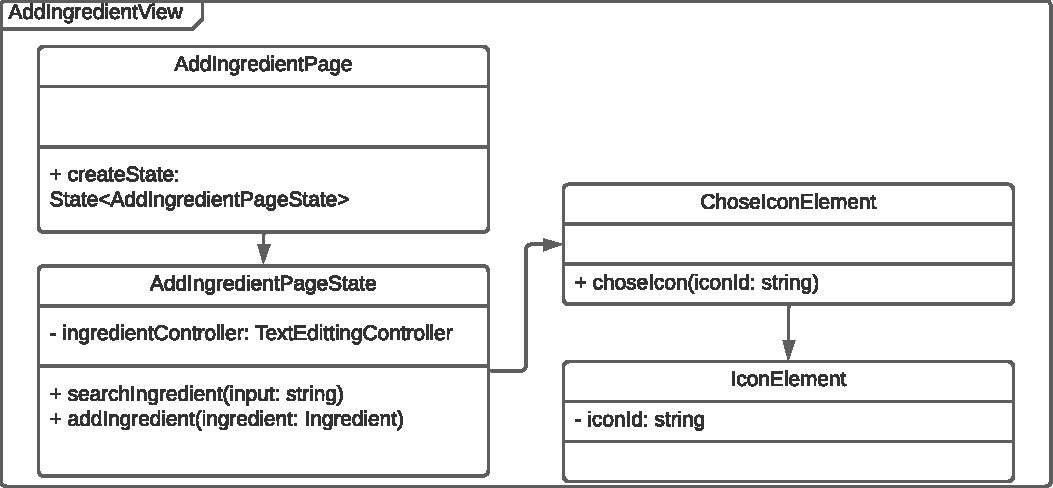
\includegraphics[width=0.95\textwidth]{images/Presentation-layer/IngredientPickerViewClass.pdf}
        \caption{Klassen für Zutaten-Auswahl-Ansicht}
    \end{minipage}
\end{figure}

\newpage

\subsection{Verwaltungsansicht}
Die Klassen beinhalten alle nötigen Funktionen und Attribute um die Verwaltungsansicht darzustellen.

\subsubsection{SettingsPage}\label{sec:SettingsPage}
\subsubsection*{Methode}
\paragraph*{createState: State<SettingsPageState>} Der Konstruktor für den SettingsPageState.

\subsubsection{SettingsPageState}\label{sec:SettingsPageState}
\subsubsection*{Attribute}
\paragraph*{newUsernameController: TextEdittingController} Die eingegebene Zeichenkette für den neuen Nutzernamen des Benutzers.

\subsubsection*{Methode}
\paragraph*{setProfileImage(image: Image)} Überprüft das Hochgeladene Bild und ruft die Funktion setProfileImage() im UserService auf.
\paragraph*{removeProfileImage()} Ruft die Funktion removeProfileImage() im UserService auf.
\paragraph*{setUserName(value: string)} Überprüft die Eingabe und ruft die Funktion setUserName() im UserService auf.
\paragraph*{joinGroup()} Die Gruppen-Beitritts-Ansicht wird aufgerufen.
\paragraph*{recipeCreationView()} Die Rezept-Erstellungs-Ansicht wird aufgerufen.
\paragraph*{deleteAccount()} Das ConfirmationElement wird aufgerufen und bei positiver Rückmeldung wird die Funktion deleteAccount() im UserService wird aufgerufen. Bei negativer Rückmeldung ändert sich nichts.

\subsubsection{LogoutButton}\label{sec:LogoutButton}
\subsubsection*{Methode}
\paragraph*{logout()} Die Funktion logout() im UserService wird aufgerufen.

\subsubsection*{GroupElement}\label{sec:GroupElement}
\subsubsection*{Attribute}
\paragraph*{group: Group} Die darzustellende Gruppe.

\subsubsection*{Methode}
\paragraph*{GroupElement(required group: Group)} Der Konstruktor für ein GroupElement. Der Parameter muss angegeben werden.
\paragraph*{leaveGroup()} Das ConfirmationElement wird aufgerufen und bei positiver Rückmeldung wird die Funktion leaveGroup() im GroupService wird aufgerufen. Bei negativer Rückmeldung ändert sich nichts.
\paragraph*{groupeDetailView()} Die Gruppen-Detail-Ansicht wird aufgerufen.

\subsubsection*{RecipeElement (\ref{sec:RecipeElement})}

\subsubsection*{ConfirmationElement (\ref{sec:ConfirmationElement})}

\subsubsection*{ReturnButton (\ref{sec:ReturnButton})}

\subsubsection*{AppBar (\ref{sec:AppBar})}

\begin{figure}[htp]

    \begin{minipage}
        [t]{0.49\textwidth}
        \centering
        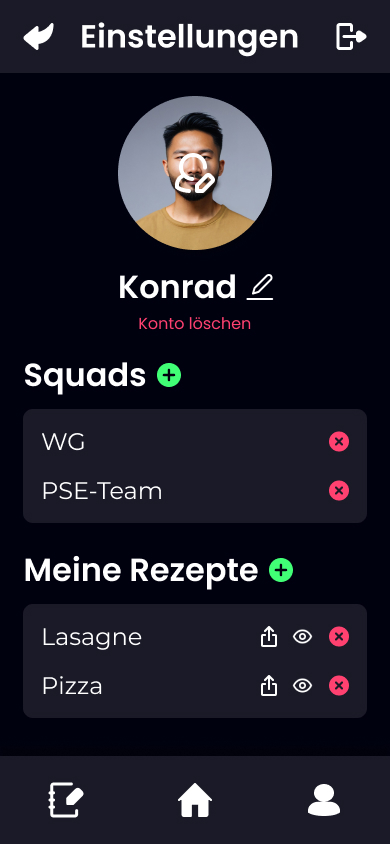
\includegraphics[height=80mm]{images/Presentation-layer/SettingsView.jpg}
        \caption{Verwaltungsansicht}
    \end{minipage}
    \begin{minipage}
        [t]{0.49\textwidth}
        \centering
        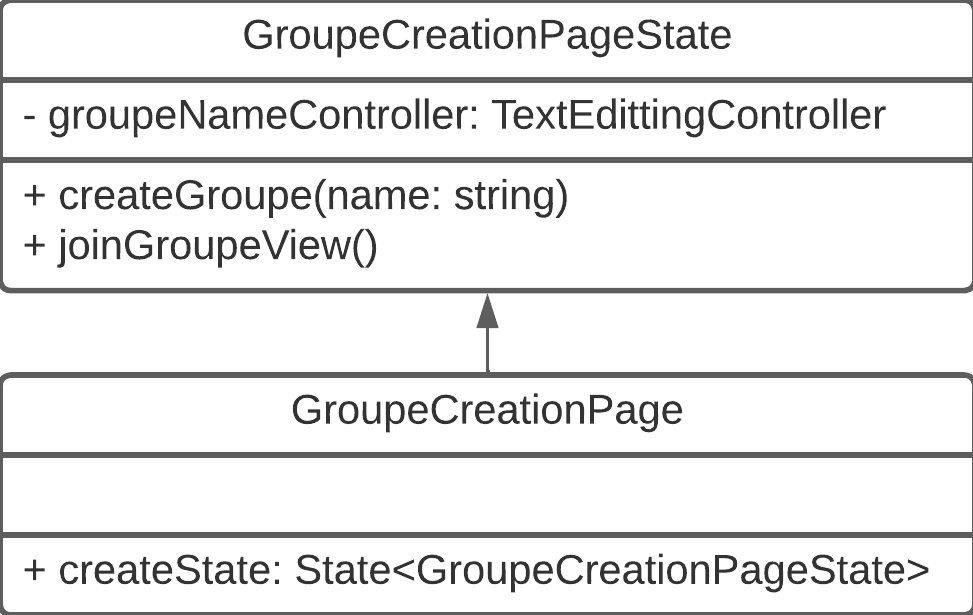
\includegraphics[width=0.95\textwidth]{images/Presentation-layer/GroupCreationViewClass.png}
        \caption{Klassen für Verwaltungsansicht}
    \end{minipage}
\end{figure}

\newpage

\subsection{QR-Code-Ansicht}
Die Klassen beinhalten alle nötigen Funktionen und Attribute um die QR-Code-Ansicht darzustellen.

\subsubsection{QrCodePage}\label{sec:QrCodePage}
\subsubsection*{Attribute}
\paragraph*{group: Group}

\subsubsection*{Methode}
\paragraph*{QrCodePage(required group: Group)} Der Konstruktor für eine QrCodePage. Der Parameter muss angegeben werden.

\subsubsection*{ReturnButton (\ref{sec:ReturnButton})}

\subsubsection*{AppBar (\ref{sec:AppBar})}


\begin{figure}[htp]
    \begin{minipage}
        [t]{0.49\textwidth}
        \centering
        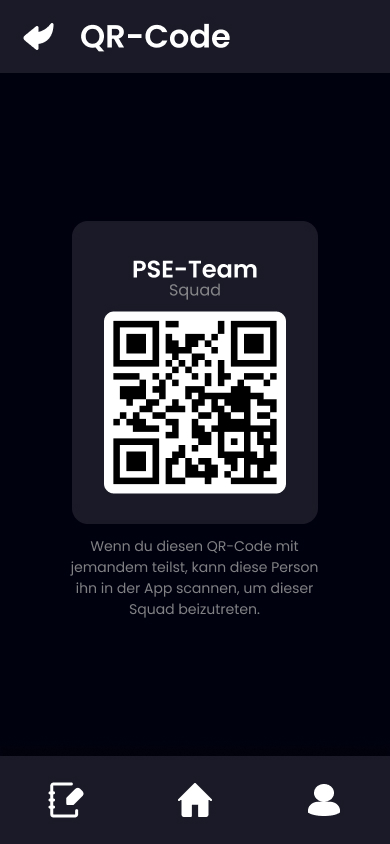
\includegraphics[height=80mm]{images/Presentation-layer/QRCodeView.jpg}
        \caption{QR-Code-Ansicht}
    \end{minipage}
    \begin{minipage}
        [t]{0.49\textwidth}
        \centering
        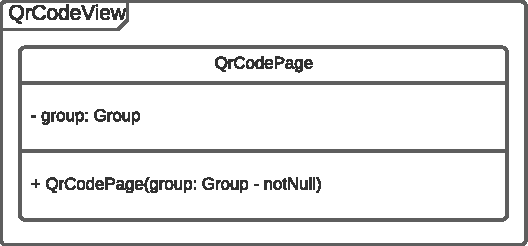
\includegraphics[width=0.95\textwidth]{images/Presentation-layer/QRCodeViewClass.pdf}
        \caption{Klassen für QR-Code-Ansicht}
    \end{minipage}
\end{figure}
\newpage

\newpage

\section{REST-Webserver}
Um seinen Account zu verwalten, Rezepte aufzurufen oder mit Gruppe interagieren zu können benötigt man die Verbindung zum Server.
Um die Anfragen performant und flexibel zu gestalten, verwendet das Projekt Node.js in Verbindung mit dem Express.js Framework.
Express.js ermöglicht es einfach einen robusten Webservice zu entwickeln. Dazu bietet Express.js eine Menge an Dienstprogrammmethoden an um das ganze zu ermöglichen.
Als Programmiersprache verwenden wir Serverseitig TypeScript. Typescript ist eine freie und quelloffene Programmiersprache, die statische Typisierung zu JavaScript hinzufügt.
Das ermöglicht es Sprachkonstrukte wie Klassen, Vererbungen und Module zu verwenden um unser Projekt sowohl client- als auch serverseitig objektorientiert zu entwickeln.
Das machte es einfacher den Aufbau des Servers zu strukturieren und auf Langzeit Wartbarkeit zu garantieren. Mit TypeScript als eines der meistgenutzten Programmiersprachen und Node.js als eines der meist beliebtesten Technologien wollen wir zudem eine hohe Zukunftssicherheit mit unserer Wahl garantieren.

\begin{figure}[htp]
    \centering
    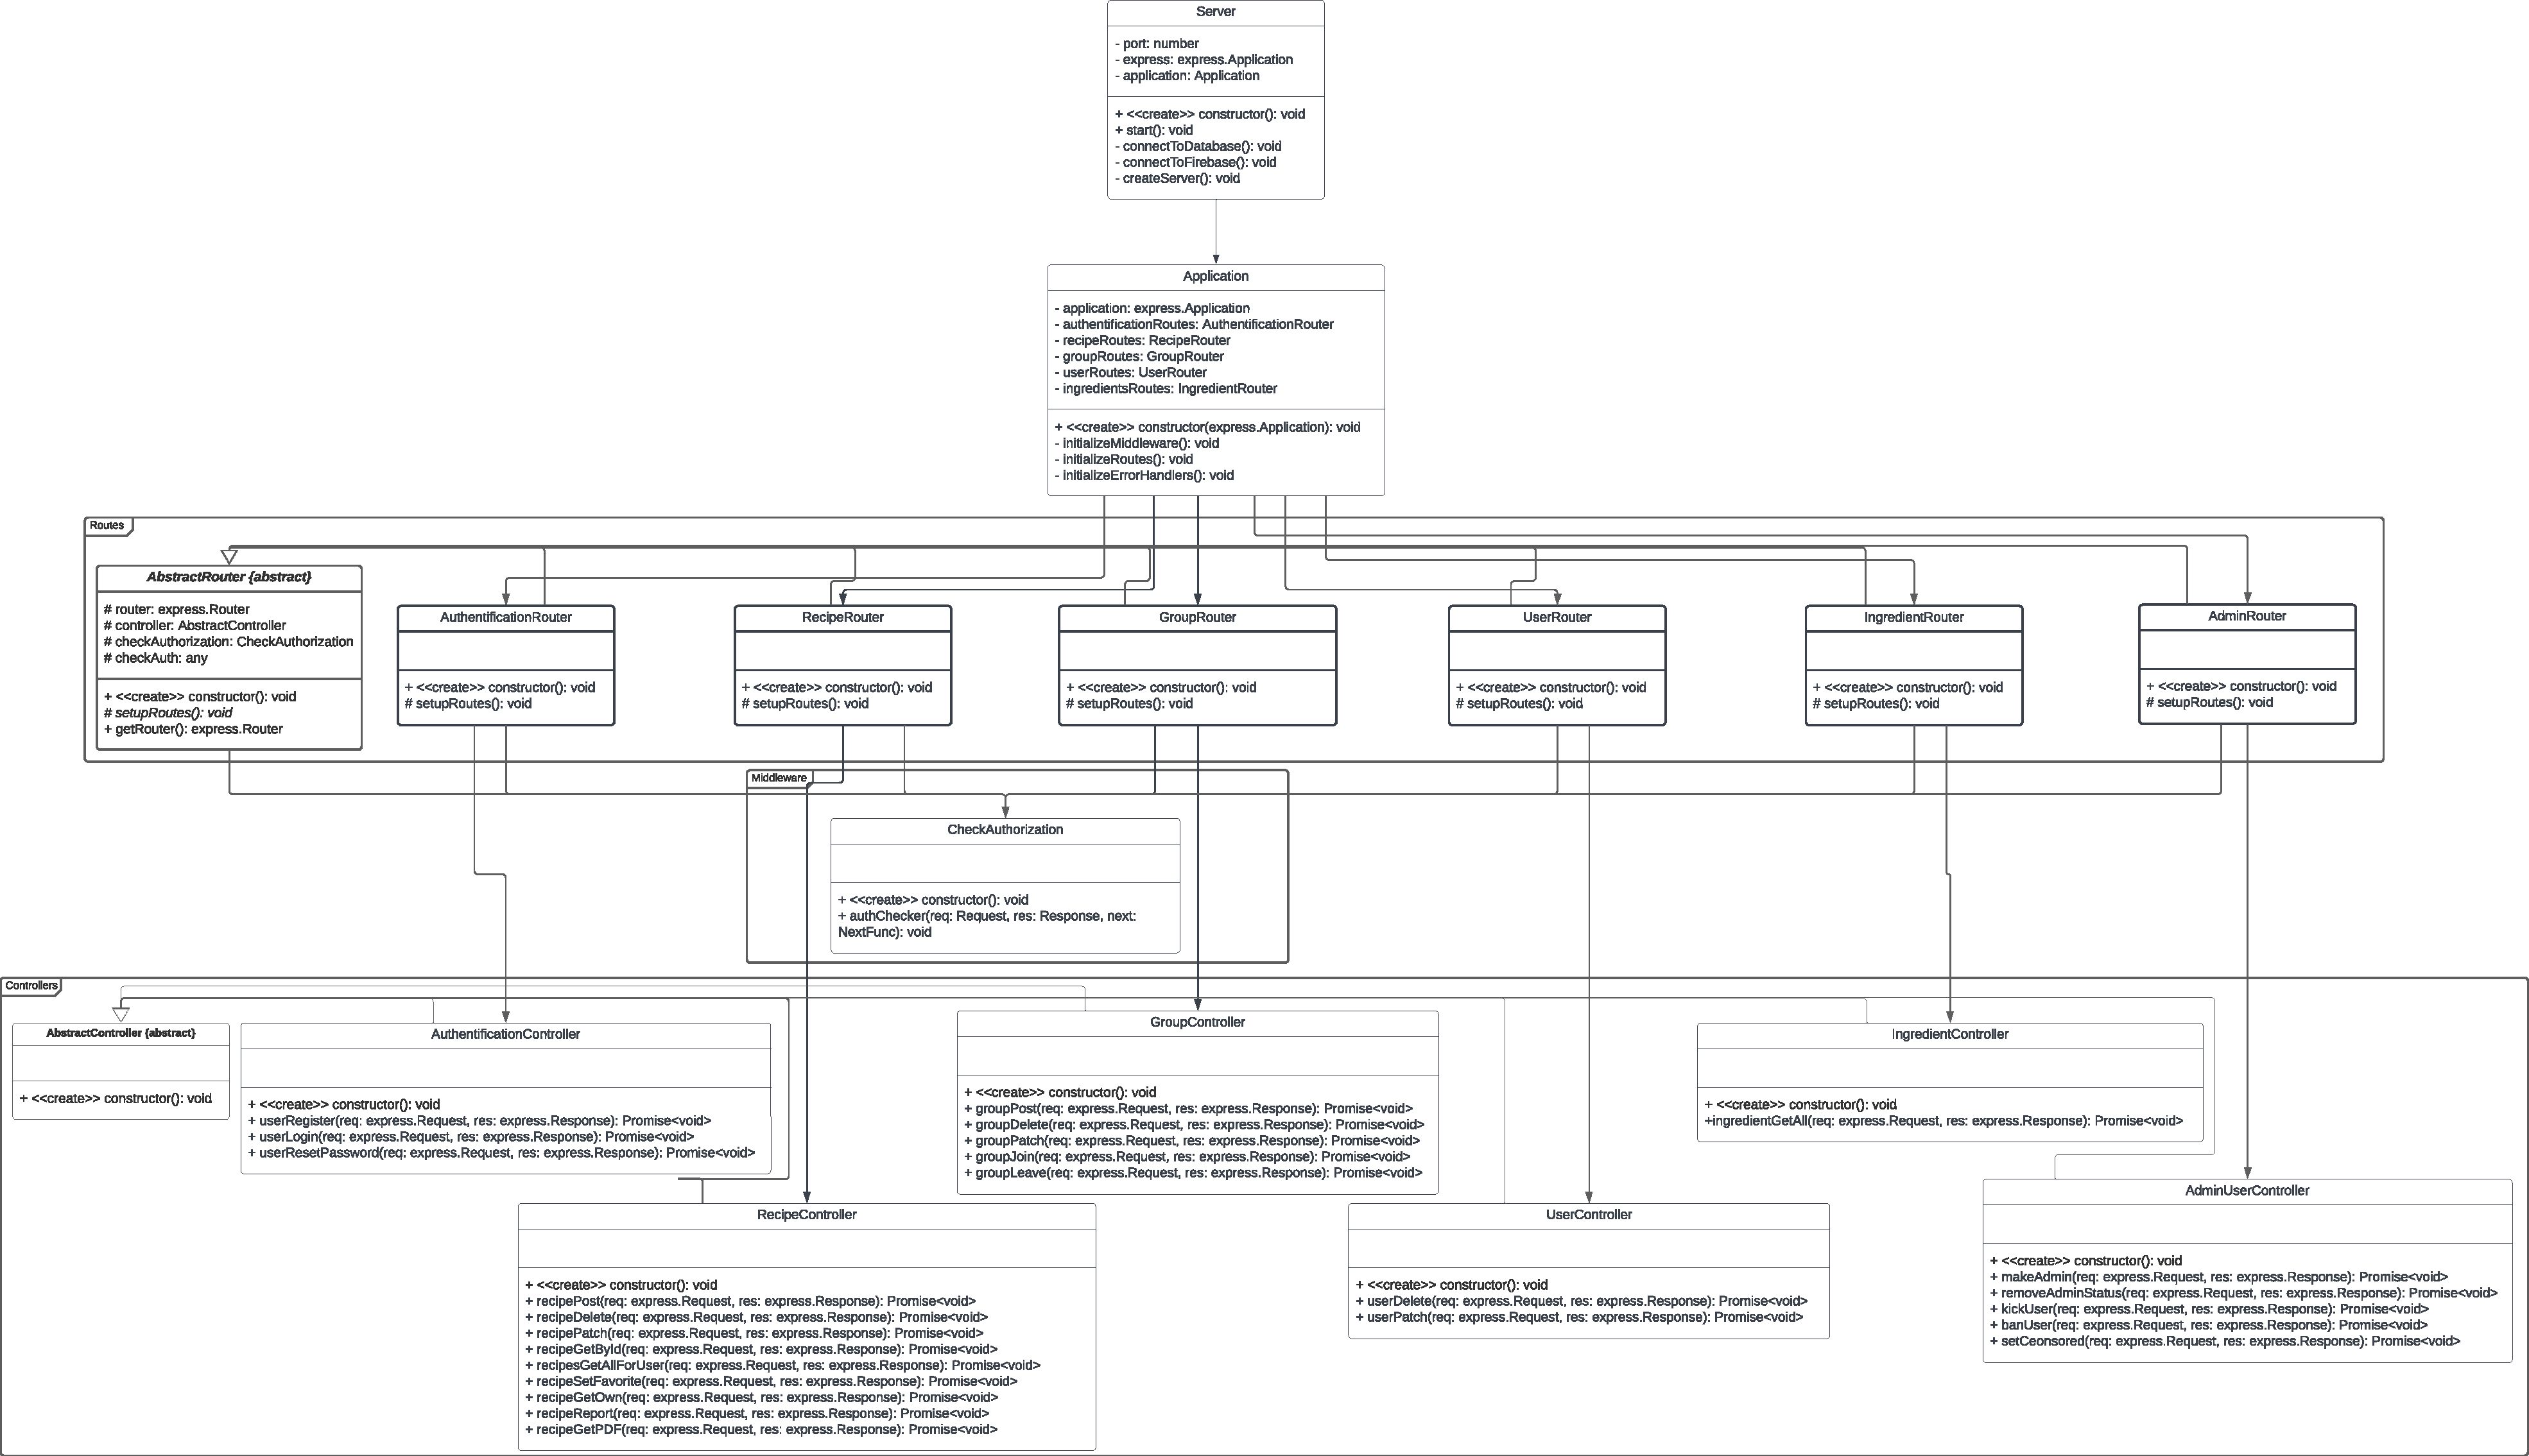
\includegraphics[width = 1\textwidth]{images/webserver/webserver.pdf}
    \caption{Klassendiagramm des Webservers}
    \label{fig:webserver}
\end{figure}

\newpage

\subsection{\texttt{Server}}\label{sec:Server}
In einer Express-Anwendung bezieht sich der Begriff "Server" auf den Hauptkomponente, die die Anfragen von Clients empfängt.
Der Server ist dafür verantwortlich die Verbindung mit der Datenbank und Firebase (siehe Nutzerverwaltung) aufzubauen und die Application zu starten.
% TODO Referenz Nutzerverwaltung

\begin{figure}[htp]
    \centering
    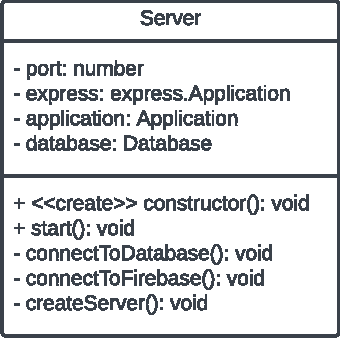
\includegraphics[width = 0.3\textwidth]{images/webserver/server.pdf}
    \caption{Klasse Server des Webservers}
    \label{fig:server}
\end{figure}

\subsection*{Attribute}
\paragraph{\texttt{port: number}}
Durch das Attribut \texttt{port} lässt sich einstellen auf welchen Port Anfragen an den Server zulässig sind. Es soll möglich sein, die Wahl des Ports durch eine Umgebungsvariable zu wählen. Wird kein Port durch eine Umgebungsvariable definiert, so soll der Server über den Port 3000 erreichbar sein.
\texttt{Port} ist vom Type number.
\paragraph{\texttt{express: express.Application}}
Express repräsentiert die Express Applikation die beim Start durch \texttt{express.listen()} Anfragen an den Port annimmt.
Express ist vom Typ express.Application. Es handelt sich um ein privates Attribut.
\paragraph{\texttt{application: Application}}
Application vom Typ Application repräsentiert das nach dem Start erzeugte Objekt der Klasse Application.

\subsection*{Methode}
\paragraph{\texttt{<<create>> constructor(): void}}
Konstruktor der Klasse Server, die beim Starten des Servers aufgerufen wird um ein neues Objekt der Klasse Server zu erzeugen. Der Konstruktor gibt keinen Wert zurück.
\paragraph{\texttt{start(): void}}
Durch Aufruf der Funktion \texttt{start()} wird der Server gestartet. Dazu wird im inneren der Funktion die privaten Funktionen \texttt{connectToDatabase()}, \texttt{connectToFirebase()} und \texttt{createServer()} aufgerufen.
\paragraph{\texttt{connectToDatabase(): boolean}}
Diese Funktion wird benötigt um die Verbindung der Datenbank herzustellen. Bei erfolgreicher Verbindung wir \texttt{true} zurückgegeben.
\paragraph{\texttt{connectToFirebase(): boolean}}
Durch diese Funktion wird die Verbindung mit Firebase aufgebaut. Bei erfolgreicher Verbindung wird \texttt{true} zurückgegeben.
\paragraph{\texttt{createServer(): boolean}}
Beim Aufrufen der create Server Funktion wird eine die der der Server mithilfe von \texttt{express.listen()} gestartet. Beim erfolgreichen Starten des Servers wird \texttt{true} zurückgegeben.

\newpage

\subsection{\texttt{Application}}\label{sec:Application}
Die Application-Klasse wird durch den Aufruf von \texttt{express()} erstellt, der eine neue Express-Anwendung erzeugt. Dieses \texttt{express()}-Objekt enthält eine Reihe von Methoden, die verwendet werden können, um Routen, Middleware und andere Funktionen zu definieren, die für den Betrieb der Anwendung erforderlich sind.

\begin{figure}[htp]
    \centering
    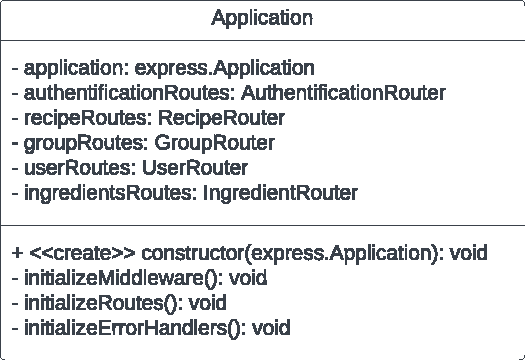
\includegraphics[width = 0.3\textwidth]{images/webserver/application.pdf}
    \caption{Klasse Application des Webservers}
    \label{fig:application}
\end{figure}


\subsubsection*{Attribute}
\paragraph{\texttt{application: express.Application}}
Das Attribut \texttt{application} speichert die \newline
\texttt{express.Application}, die beim erzeugen des Objekts dem Konstruktor mitgeben wird.
Durch dieses Attribut bekommt die Klasse Applikation mitgeteilt, auf welcher \texttt{express.Application} die in dieser Klasse erzeugten Routing-Punkte angewendet werden sollen.
\texttt{Application} ist vom Typ \texttt{express.Application}.
\paragraph{\texttt{authentificationRoutes: AuthentificationRouter}}
Dieses Attribut repräsentiert den \newline
\texttt{AuthentificationRouter} in der Express.js Anwendung. \texttt{AuthenthificationRouter} ist vom Typ \texttt{AuthentificationRouter}.
\paragraph{\texttt{recipeRoutes: RecipeRouter}}
Dieses Attribut repräsentiert den \texttt{RecipeRouter} in der Express.js Anwendung. \texttt{RecipeRouter} ist vom Typ \texttt{RecipeRouter}.
\paragraph{\texttt{groupRoutes: GroupRouter}}
Das Attribut für den \texttt{GroupRouter}. \texttt{groupRouter} ist vom \newline
Typ \texttt{GroupRouter}.
\paragraph{\texttt{userRoutes: UserRouter}}
Das Attribut für den \texttt{UserRouter}. \texttt{userRouter} ist vom Typ \newline
\texttt{UserRouter}.
\paragraph{\texttt{adminRouter: AdminRouter}}
Das Attribut für den \texttt{AdminRouter}. \texttt{adminRouter} ist vom Typ \texttt{AdminRouter}.
\paragraph{\texttt{ingredientRouter: IngredientRouter}}
\texttt{ingredientRouter} ist vom Typ \texttt{IngredientRouter}.
Das Attribut für den \texttt{IngredientRouter}. \newline

\subsubsection*{Methode}
\paragraph{\texttt{initializeMiddleware(): void}}
Mit dieser Methode wird die Middleware initialisiert. Hier ist es möglich die eingehenden Anfragen vorzubehandeln, bevor sie an die eigentlichen Routstellen weitergeleitet werden.
Eine Middleware die beispielsweise zwischengeschaltet werden kann wäre Morgan. Morgan ermöglicht es HTTP anfragen zu loggen.
\paragraph{\texttt{initializeRoutes(): void}}
Mit dieser Methode werden die Routen initialisiert.
\paragraph{\texttt{initializeErrorHandlers(): void}}
Mit dieser Methode Werden Error-Handler initialisiert. Diese wird benötigt, wenn beispielsweise eine Anfrage an keine gültige Route gestellt wird.

\newpage

\subsection{Router}
Ein Router kann als eine Art Zwischenschicht betrachtet werden, die HTTP-Anfragen an die entsprechenden Controller weiterleitet.
Er hilft dabei, den Code zu strukturieren und die Handhabung von Routen in einer modularen und organisierten Weise zu ermöglichen.
Ein Router in Express wird durch die Verwendung des \texttt{express.Router()}-Objekts erstellt.
Dieses Objekt stellt eine Miniaturversion der Express-Anwendung dar und kann Routen und Endpunkte definieren, ähnlich wie die Hauptanwendung.
Ein Router kann mit einem Pfad oder Präfix konfiguriert werden, der angibt, unter welchem Pfad seine Routen verfügbar sein sollen.

Ein Router kann dabei mehrere Routen definieren, indem verschiedene HTTP-Methoden wie \texttt{GET}, \texttt{POST}, \texttt{PUT}, \texttt{DELETE} usw. verwendet werden.
Jede Route kann einen oder mehrere Handler haben, die ausgeführt werden, wenn die Route mit einer Anfrage übereinstimmt.
Diese Handler sind Funktionen, die Zugriff auf die Anfrage- und Antwortobjekte haben und die erforderlichen Aktionen durchführen.
Router ermöglichen es, den Code in einer Express-Anwendung besser zu organisieren, indem sie verwandte Routen und deren Handler gruppieren.
Dies erleichtert die Wartung, Skalierbarkeit und Lesbarkeit des Codes.

\begin{figure}[htp]
    \centering
    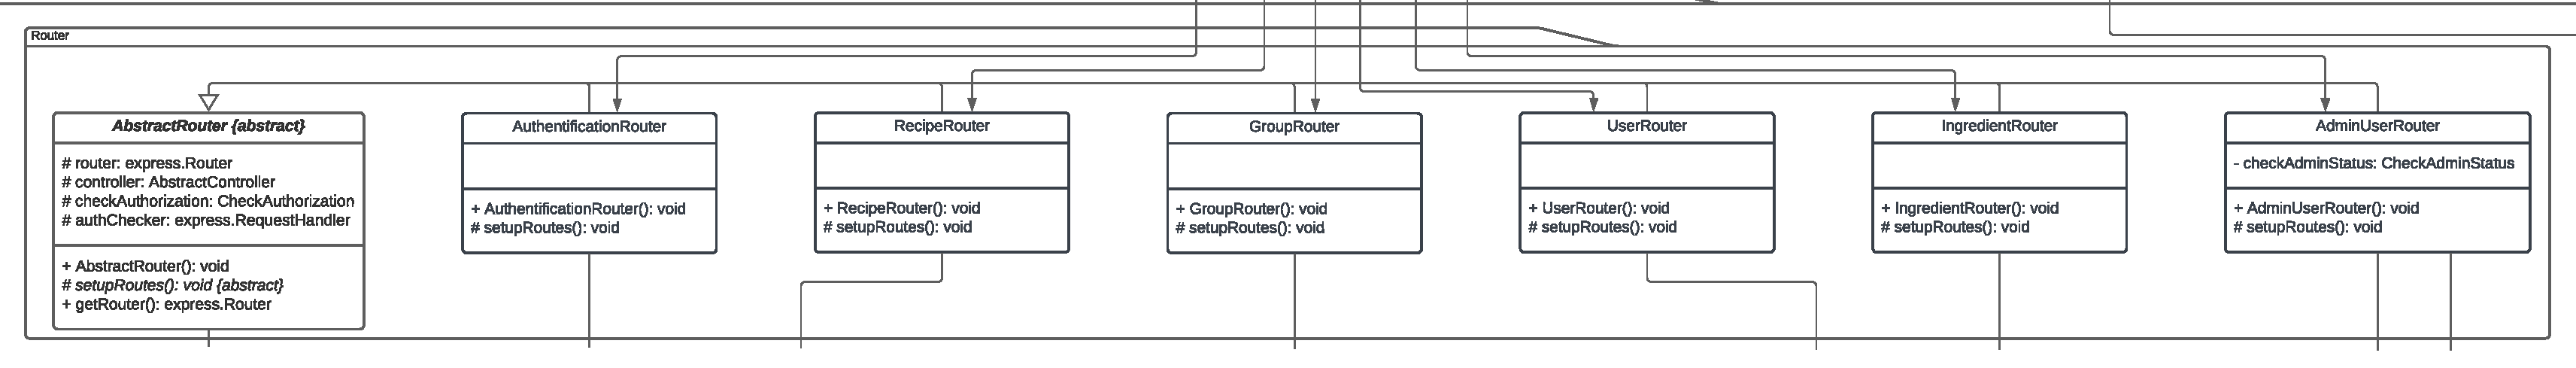
\includegraphics[width = 1\textwidth]{images/webserver/router.pdf}
    \caption{Router-Klassen des Webservers}
    \label{fig:router}
\end{figure}

\subsubsection{\texttt{AbstractRouter}}\label{sec:AbstractRouter}
Der \texttt{AbstractRouter} ist eine abstrakte Repräsentation eines Routers. So kann ein grundlegender Aufbau für alle Router garantiert werden. Alle Router erben von dieser Klasse \texttt{AbstractRouter}.
\subsubsection*{Attribute}
\paragraph{\texttt{router: express.Router}}
Attribut, dass einen Router in Express repräsentiert. Das zugehörige Objekt soll beim Konstruktoraufruf erzeugt werden. 
\paragraph{\texttt{controller: AbstractController}}
Attribut, dass einen abstrakten Controller repräsentiert. Mit diesem Attribut wird in den jeweiligen Routern der dazu passende Controller gespeichert.
\paragraph{\texttt{checkAuthorization: CheckAuthorization}} % TODO
\paragraph{\texttt{checkAuth: any}} % TODO Datentyp

\subsubsection*{Methoden}
\paragraph{\texttt{abstract setupRoutes(): void}}
Diese abstrakte Methode definiert einen Methode die die Kinderklassen implementieren müssen.
\paragraph{\texttt{getRouter(): express.Router}}
Getter-Methode für das Attribut \texttt{router}.


\subsubsection{\texttt{AuthentificationRouter}}\label{sec:AuthentificationRouter}
Der \texttt{AuthentificationRouter} ist speziell für die Verarbeitung von Authentifizierungsanfragen zuständig.
\subsubsection*{Methoden}
\paragraph{\texttt{setupRoutes(): void}}
Mit dieser Methode werden die Handler im jeweiligen Controller den zugehörigen Routestellen zugewiesen.

\subsubsection{\texttt{RecipeRouter}}\label{sec:RecipeRouter}
Der \texttt{RecipeRouter} ist für die Verwaltung der Routen und Endpunkte verantwortlich, die mit Rezepten zusammenhängen.
\subsubsection*{Methoden}
\texttt{RecipeRouter}.
\paragraph{\texttt{setupRoutes(): void}}
Mit dieser Methode werden die Handler im jeweiligen Controller den zugehörigen Routestellen zugewiesen.

\subsubsection{\texttt{GroupRouter}}\label{sec:GroupRouter}
Der \texttt{GroupRouter} ist verantwortlich für die Verwaltung der Routen und Endpunkte, die mit Gruppen in der Anwendung zusammenhängen.
\subsubsection*{Methoden}
\paragraph{\texttt{setupRoutes(): void}}
Mit dieser Methode werden die Handler im jeweiligen Controller den zugehörigen Routestellen zugewiesen.

\subsubsection{\texttt{UserRouter}}\label{sec:UserRouter}
Der \texttt{UserRouter} ist für die Verwaltung von Routen und Endpunkten zuständig, die mit Benutzeraktionen und -informationen zusammenhängen.
\subsubsection*{Methode}
\paragraph{\texttt{setupRoutes(): void}}
Mit dieser Methode werden die Handler im jeweiligen Controller den zugehörigen Routestellen zugewiesen.

\subsubsection{\texttt{IngredientRouter}}\label{sec:IngredientRouter}
Der \texttt{IngredientRouter} ist verantwortlich für die Verwaltung von Routen und Endpunkten, die mit Zutaten in der Anwendung zusammenhängen.
\subsubsection*{Methoden}
\paragraph{\texttt{setupRoutes(): void}}
Mit dieser Methode werden die Handler im jeweiligen Controller den zugehörigen Routestellen zugewiesen.

\subsubsection{\texttt{AdminUserRouter}}\label{sec:AdminUserRouter}
Der \texttt{AdminUserRouter} ist verantwortlich für die Verwaltung von Routen und Endpunkten, die mit Administrator Interaktionen zusammenhängen.
\subsubsection*{Methoden}
\paragraph{\texttt{setupRoutes(): void}}
Mit dieser Methode werden die Handler im jeweiligen Controller den zugehörigen Routestellen zugewiesen.

\newpage

\subsection{Middleware}
Durch die Middleware können Anfragen vorher bearbeitet werden, bevor sie zu den eigentlichen Routingstellen gehen.

\begin{figure}[htp]
    \centering
    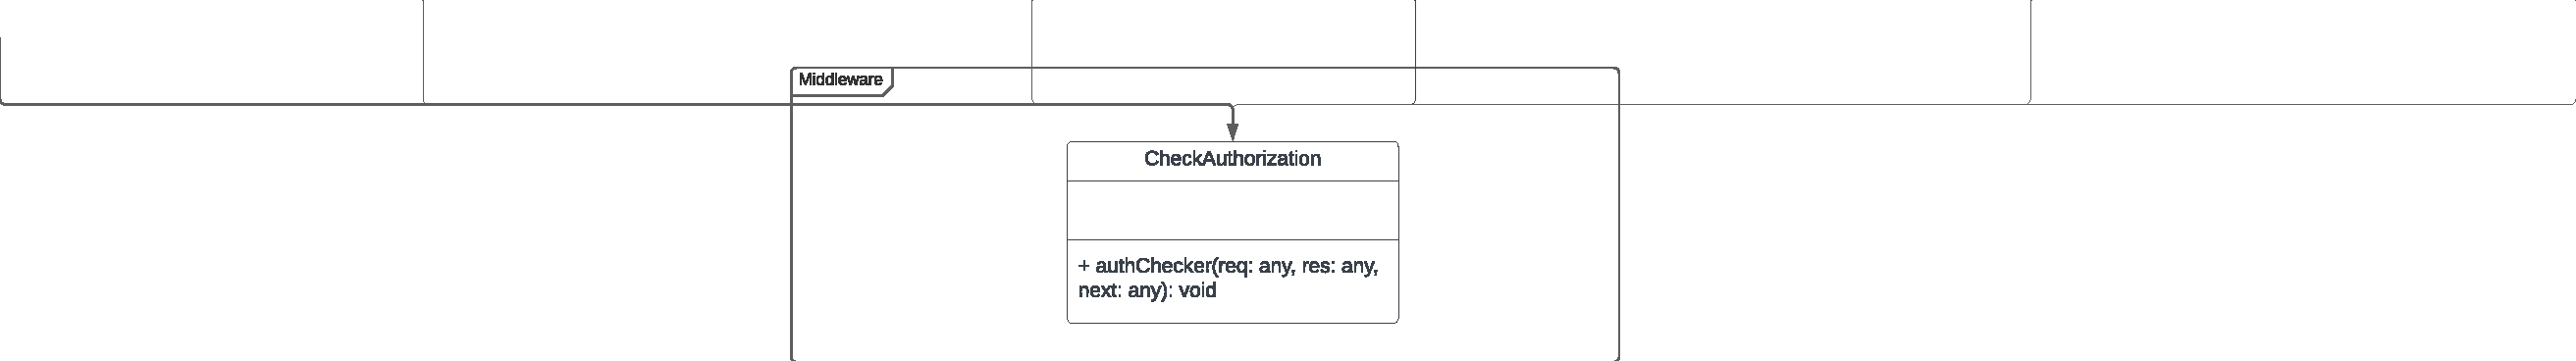
\includegraphics[width = 1\textwidth]{images/webserver/middleware.pdf}
    \caption{Middleware-Klassen des Webservers}
    \label{fig:middleware}
\end{figure}

\subsubsection{\texttt{CheckAuthorization}}\label{sec:CheckAuthorization}
Mit \texttt{CheckAuthorization} kann vor einer Anfrage an einen Router gescheckt werde, ob die Anfrage von Nutzer mit validen Firebase Id Token kommt. % Referenz Nutzerverwaltung mit Firebase
\subsubsection*{Methoden}
\paragraph{\texttt{authChecker(req: express.Request, res: express.Response, next: express.NextFunction): void}}
Mit dieser Methode wird durch eine Abfrage an Firebase überprüft, ob das Id Token valide ist.

\newpage

\subsection{Controller}
In einer Express-Anwendung bezieht sich der Begriff "Controller" auf eine Komponente oder eine Sammlung von Funktionen, die dazu dienen, die Logik für bestimmte Routen oder Endpunkte zu implementieren.
Der Controller ist für die Verarbeitung von Anfragen zuständig, die an eine bestimmte Route gesendet werden, und für die Rückgabe von entsprechenden Antworten.
Der Controller agiert als eine Art Vermittler zwischen den Routen und der eigentlichen Geschäftslogik der Anwendung.
Ein Controller ist ein Objekt, das Handler-Funktionen für verschiedene Routen bereitstellt.
Diese Handler-Funktionen werden als Callback-Funktionen für die entsprechenden Routen registriert und nehmen die Anfrage (\texttt{req}) und die Antwort (\texttt{res}) als Parameter entgegen.



\begin{figure}[htp]
    \centering
    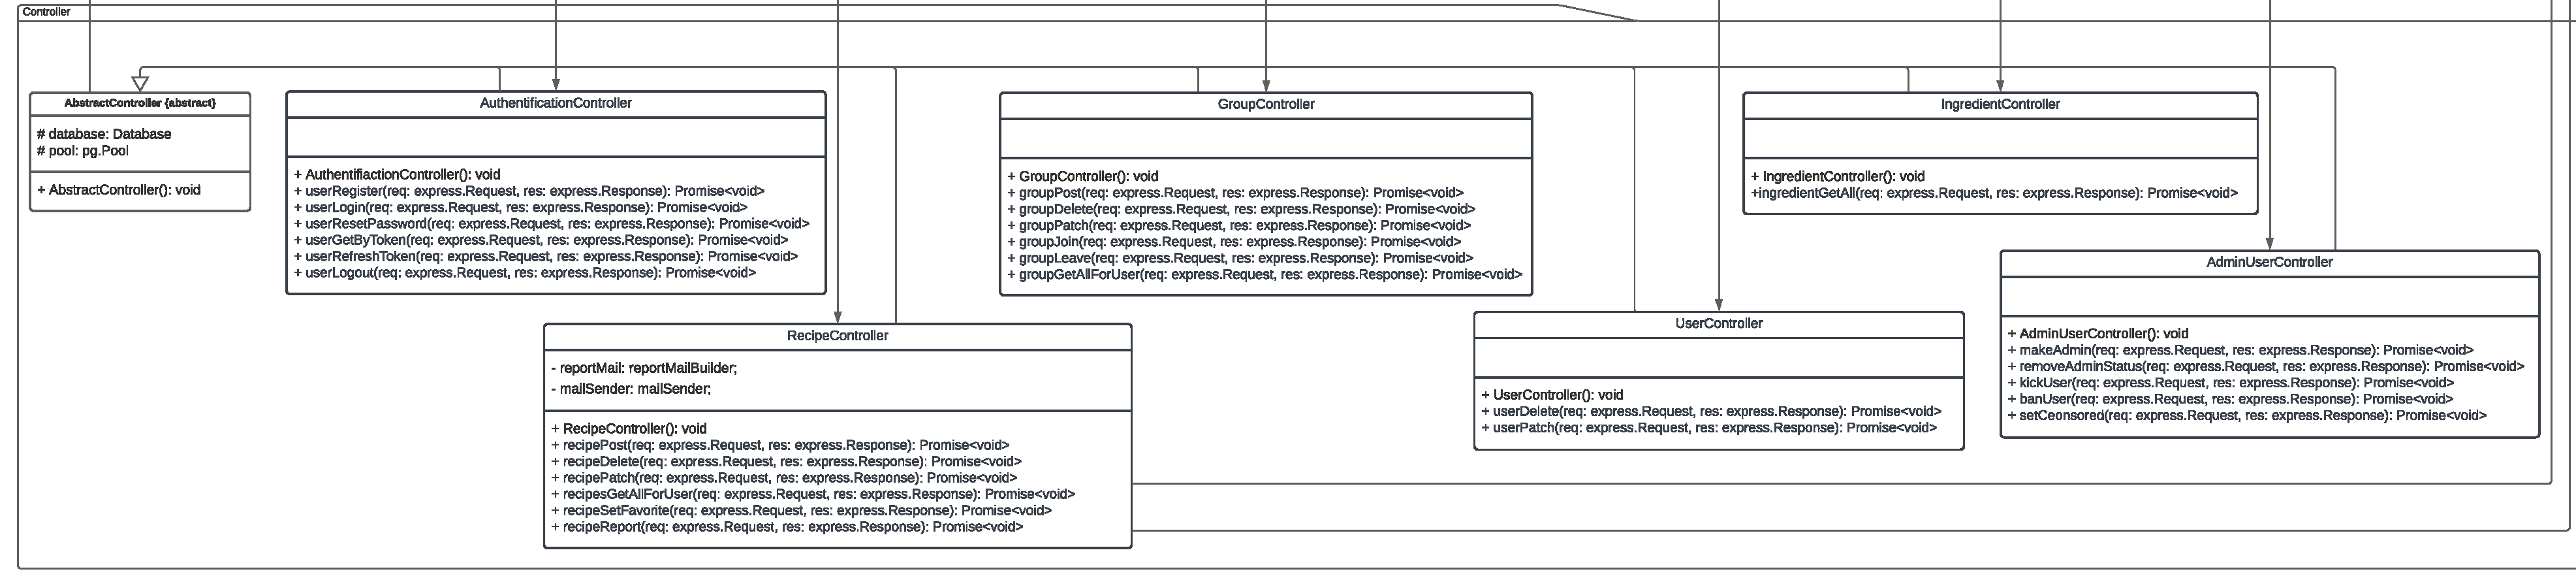
\includegraphics[width = 1\textwidth]{images/webserver/controller.pdf}
    \caption{Controller Klassen des Webservers}
    \label{fig:controller}
\end{figure}

\subsubsection{\texttt{AbstractController}}\label{sec:AbstractController}
Der \texttt{AbstractController} beschreibt ein abstrakte Darstellung eines Controllers. Alle Controller erben von dieser Klasse.

\subsubsection{\texttt{AuthentificationController}}\label{sec:AuthentificationController}
Der \texttt{AuthentificationController} ist verantwortlich für alle Anfragen, die mit der Nutzerverwaltung in Firebase direkt etwas zu zun haben. Das heißt konkret das Registrieren, Einloggen und Passwort zurücksetzen des Nutzers.
\subsubsection*{Methoden}
\paragraph{\texttt{public userRegister(req: express.Request, res: express.Response): void}}

Diese Methode sorgt dafür, dass der Nutzer sich registrieren kann. Der \texttt{req}-Parameter enthält Informationen über den eingehenden HTTP-Request, der Daten wie Benutzername, Passwort und andere Informationen übermittelt. Der \texttt{res}-Parameter wird verwendet, um eine Antwort auf den Request zu senden, beispielsweise um dem Benutzer mitzuteilen, ob die Registrierung erfolgreich war oder Fehler aufgetreten sind.
\paragraph{\texttt{public userLogin(req: express.Request, res: express.Response): void}}
Diese Methode sorgt dafür, dass der Nutzer sich einloggen kann. Der \texttt{req}-Parameter enthält Informationen über den eingehenden HTTP-Request, der Daten wie Benutzername, Passwort und andere Informationen übermittelt. Der \texttt{res}-Parameter wird verwendet, um eine Antwort auf den Request zu senden, beispielsweise um dem Benutzer mitzuteilen, ob das Einloggen erfolgreich war oder Fehler aufgetreten sind. 
\paragraph{\texttt{userResetPassword(req: express.Request, res: express.Response): void}}
Diese Methode sorgt dafür, dass der Nutzer sein Passwort zurücksetzen lassen kann. Der \texttt{req}-Parameter enthält Informationen über den eingehenden HTTP-Request, der Daten wie Benutzername übermittelt. Der \texttt{res}-Parameter wird verwendet, um eine Antwort auf den Request zu senden, beispielsweise um dem Benutzer mitzuteilen, ob die Anfrage zum Passwort zurücksetzen erfolgreich war oder Fehler aufgetreten sind. 

\subsubsection{\texttt{RecipeController}}\label{sec:RecipeController}
Der \texttt{RecipeController} ist verantwortlich für alle Anfragen, die mit den Rezepten zu tun haben.
\subsubsection*{Methode}
\paragraph{\texttt{recipePost(req: express.Request, res: express.Response): Promise<void>}}
Mit der Methode \texttt{recipePost} kann ein neues Rezept erstellt werden und in der Datenbank gespeichert werden. Der \texttt{req}-Parameter enthält Informationen über den eingehenden HTTP-Request, der Daten wie Rezeptname, Rezeptbeschreibung, Zutaten, Zubereitung und andere Informationen übermittelt. Der \texttt{res}-Parameter wird verwendet, um eine Antwort auf den Request zu senden, beispielsweise um dem Benutzer mitzuteilen, ob das Erstellen des Rezepts erfolgreich war oder Fehler aufgetreten sind.
Der Rückgabewert ist vom Typ \texttt{Promise<void>}, da die Funktion asynchron ausgeführt wird.
\paragraph{\texttt{recipeDelete(req: express.Request, res: express.Response): Promise<void>}}
Mit der Methode \texttt{recipeDelete} kann ein Rezept gelöscht werden. Der \texttt{req}-Parameter enthält Informationen über den eingehenden HTTP-Request, der Daten wie Rezeptname, Rezeptbeschreibung, Zutaten, Zubereitung und andere Informationen übermittelt. Der \texttt{res}-Parameter wird verwendet, um eine Antwort auf den Request zu senden, beispielsweise um dem Benutzer mitzuteilen, ob das Löschen des Rezepts erfolgreich war oder Fehler aufgetreten sind.
Der Rückgabewert ist vom Typ \texttt{Promise<void>}, da die Funktion asynchron ausgeführt wird.
\paragraph{\texttt{recipePatch(req: express.Request, res: express.Response): Promise<void>}}
Diese Methode sorgt dafür, dass ein Rezept bearbeitet werden kann. Der \texttt{req}-Parameter enthält Informationen über den eingehenden HTTP-Request, der Daten wie Rezeptname, Rezeptbeschreibung, Zutaten, Zubereitung und andere Informationen übermittelt. Der \texttt{res}-Parameter wird verwendet, um eine Antwort auf den Request zu senden, beispielsweise um dem Benutzer mitzuteilen, ob das Bearbeiten des Rezepts erfolgreich war oder Fehler aufgetreten sind.
Der Rückgabewert ist vom Typ \texttt{Promise<void>}, da die Funktion asynchron ausgeführt wird.
\paragraph{\texttt{recipeGetById(req: express.Request, res: express.Response): Promise<void>}}
Durch die Methode \texttt{recipeGetById} kann ein Rezept anhand seiner Id abgerufen werden. Der \texttt{req}-Parameter enthält Informationen über den eingehenden HTTP-Request, der Daten wie Rezeptname, Rezeptbeschreibung, Zutaten, Zubereitung und andere Informationen übermittelt. Der \texttt{res}-Parameter wird verwendet, um eine Antwort auf den Request zu senden, beispielsweise um dem Benutzer mitzuteilen, ob das Abrufen des Rezepts erfolgreich war oder Fehler aufgetreten sind.
Der Rückgabewert ist vom Typ \texttt{Promise<void>}, da die Funktion asynchron ausgeführt wird.
\paragraph{\texttt{recipesGetAllForUser(req: express.Request, res: express.Response): Promise<void>}}
Mit der Methode \texttt{recipesGetAllForUser} können alle Rezepte eines Nutzers abgerufen werden. Der \texttt{req}-Parameter enthält Informationen über den eingehenden HTTP-Request, der Daten wie Rezeptname, Rezeptbeschreibung, Zutaten, Zubereitung und andere Informationen übermittelt. Der \texttt{res}-Parameter wird verwendet, um eine Antwort auf den Request zu senden, beispielsweise um dem Benutzer mitzuteilen, ob das Abrufen der Rezepte erfolgreich war oder Fehler aufgetreten sind.
Der Rückgabewert ist vom Typ \texttt{Promise<void>}, da die Funktion asynchron ausgeführt wird.
\paragraph{\texttt{recipeSetFavorite(req: express.Request, res: express.Response): Promise<void>}}
Durch die Methode \texttt{recipeSetFavorite} kann ein Rezept als Favorit markiert werden. Der \texttt{req}-Parameter enthält Informationen über den eingehenden HTTP-Request, der Daten wie Rezept Id und andere Informationen übermittelt. Der \texttt{res}-Parameter wird verwendet, um eine Antwort auf den Request zu senden, beispielsweise um dem Benutzer mitzuteilen, ob das Markieren des Rezepts als Favorit erfolgreich war oder Fehler aufgetreten sind.
Der Rückgabewert ist vom Typ \texttt{Promise<void>}, da die Funktion asynchron ausgeführt wird.
\paragraph{\texttt{recipeGetOwn(req: express.Request, res: express.Response): Promise<void>}}
Mit der Methode \texttt{recipeGetOwn} können alle Rezepte eines Nutzers abgerufen werden. Der \texttt{req}-Parameter enthält Informationen über den eingehenden HTTP-Request, der Daten wie Rezeptname, Rezeptbeschreibung, Zutaten, Zubereitung und andere Informationen übermittelt. Der \texttt{res}-Parameter wird verwendet, um eine Antwort auf den Request zu senden, beispielsweise um dem Benutzer mitzuteilen, ob das Abrufen der Rezepte erfolgreich war oder Fehler aufgetreten sind.
Der Rückgabewert ist vom Typ \texttt{Promise<void>}, da die Funktion asynchron ausgeführt wird.
\paragraph{\texttt{recipeReport(req: express.Request, res: express.Response): Promise<void>}}
Mit der Methode \texttt{recipeReport} kann ein Rezept gemeldet werden. Der \texttt{req}-Parameter enthält Informationen über den eingehenden HTTP-Request, der Daten wie Rezept Id und andere Informationen übermittelt. Der \texttt{res}-Parameter wird verwendet, um eine Antwort auf den Request zu senden, beispielsweise um dem Nutzer mitzuteilen, ob das Melden des Rezepts erfolgreich war oder Fehler aufgetreten sind.
Der Rückgabewert ist vom Typ \texttt{Promise<void>}, da die Funktion asynchron ausgeführt wird.
\paragraph{\texttt{recipeGetPDF(req: express.Request, res: express.Response): Promise<void>}}
Mit der Methode \texttt{recipeGetPDF} kann ein Rezept als PDF abgerufen werden. Der \texttt{req}-Parameter enthält Informationen über den eingehenden HTTP-Request, der Daten wie Rezept Id und andere Informationen übermittelt. Der \texttt{res}-Parameter wird verwendet, um eine Antwort auf den Request zu senden, beispielsweise um dem Nutzer mitzuteilen, ob das Abrufen des Rezepts als PDF erfolgreich war oder Fehler aufgetreten sind.
Der Rückgabewert ist vom Typ \texttt{Promise<void>}, da die Funktion asynchron ausgeführt wird.


\subsubsection{\texttt{GroupController}}\label{sec:GroupController}
Der \texttt{GroupController} ist verantwortlich für alle Anfragen, die mit den Gruppen zu tun haben. Darunter fallen das Erstellen, Löschen, Bearbeiten, Beitreten und Verlassen von Gruppen.
\subsubsection*{Methode}
\paragraph{\texttt{groupPost(req: express.Request, res: express.Response): void}}
Mit der Methode \texttt{groupPost} kann eine neue Gruppe erstellt werden. Der \texttt{req}-Parameter enthält Informationen über den eingehenden HTTP-Request, der Daten wie Gruppenname, Gruppenbeschreibung und andere Informationen übermittelt. Der \texttt{res}-Parameter wird verwendet, um eine Antwort auf den Request zu senden, beispielsweise um dem Nutzer mitzuteilen, ob das Erstellen der Gruppe erfolgreich war oder Fehler aufgetreten sind.
Der Rückgabewert ist vom Typ \texttt{Promise<void>}, da die Funktion asynchron ausgeführt wird.
\paragraph{\texttt{groupDelete(req: express.Request, res: express.Response): void}}
Diese Methode sorgt dafür, dass eine Gruppe gelöscht werden kann. Der \texttt{req}-Parameter enthält Informationen über den eingehenden HTTP-Request, der Daten wie Gruppenname, Gruppenbeschreibung und andere Informationen übermittelt. Der \texttt{res}-Parameter wird verwendet, um eine Antwort auf den Request zu senden, beispielsweise um dem Nutzer mitzuteilen, ob das Löschen der Gruppe erfolgreich war oder Fehler aufgetreten sind.
Der Rückgabewert ist vom Typ \texttt{Promise<void>}, da die Funktion asynchron ausgeführt wird.
\paragraph{\texttt{groupGetById(req: express.Request, res: express.Response): void}}
Durch diese Methode kann eine Gruppe anhand ihrer Id abgerufen werden. Der \texttt{req}-Parameter enthält Informationen über den eingehenden HTTP-Request, der Daten wie Gruppenname, Gruppenbeschreibung und andere Informationen übermittelt. Der \texttt{res}-Parameter wird verwendet, um eine Antwort auf den Request zu senden, beispielsweise um dem Nutzer mitzuteilen, ob das Abrufen der Gruppe erfolgreich war oder Fehler aufgetreten sind.
Der Rückgabewert ist vom Typ \texttt{Promise<void>}, da die Funktion asynchron ausgeführt wird.
\paragraph{\texttt{groupPatch(req: express.Request, res: express.Response): void}}
Diese Methode sorgt dafür, dass eine Gruppe bearbeitet werden kann. Der \texttt{req}-Parameter enthält Informationen über den eingehenden HTTP-Request, der Daten wie Gruppenname, Gruppenbeschreibung und andere Informationen übermittelt. Der \texttt{res}-Parameter wird verwendet, um eine Antwort auf den Request zu senden, beispielsweise um dem Nutzer mitzuteilen, ob das Bearbeiten der Gruppe erfolgreich war oder Fehler aufgetreten sind.
Der Rückgabewert ist vom Typ \texttt{Promise<void>}, da die Funktion asynchron ausgeführt wird.
\paragraph{\texttt{groupJoin(req: express.Request, res: express.Response): void}}
Mit der Methode \texttt{groupJoin} kann ein Nutzer einer Gruppe beitreten. Der \texttt{req}-Parameter enthält Informationen über den eingehenden HTTP-Request, der Daten wie Gruppen Id und andere Informationen übermittelt. Der \texttt{res}-Parameter wird verwendet, um eine Antwort auf den Request zu senden, beispielsweise um dem Nutzer mitzuteilen ob das Beitreten der Gruppe erfolgreich war oder Fehler aufgetreten sind.
Der Rückgabewert ist vom Typ \texttt{Promise<void>}, da die Funktion asynchron ausgeführt wird.
\paragraph{\texttt{groupLeave(req: express.Request, res: express.Response): void}}
Mit der Methode \texttt{groupLeave} kann ein Nutzer einer Gruppe beitreten. Der \texttt{req}-Parameter enthält Informationen über den eingehenden HTTP-Request, der Daten wie Gruppen Id und andere Informationen übermittelt. Der \texttt{res}-Parameter wird verwendet, um eine Antwort auf den Request zu senden, beispielsweise um dem Nutzer mitzuteilen ob das Verlassen der Gruppe erfolgreich war oder Fehler aufgetreten sind.
Der Rückgabewert ist vom Typ \texttt{Promise<void>}, da die Funktion asynchron ausgeführt wird.

\subsubsection{\texttt{UserController}}\label{sec:UserController}
Der \texttt{UserController} ist verantwortlich für alle Anfragen, die mit den Nutzern zu tun haben, wie das ändern der Nutzerdaten oder das Löschen des Nutzers.
\subsubsection*{Methode}
\paragraph{\texttt{userDelete(req: express.Request, res: express.Response): void}}
Mit der Methode \texttt{userDelete} kann ein Nutzer gelöscht werden. Der \texttt{req}-Parameter enthält Informationen über den eingehenden HTTP-Request, der Daten wie Nutzername und andere Informationen übermittelt. Der \texttt{res}-Parameter wird verwendet, um eine Antwort auf den Request zu senden, beispielsweise um dem Nutzer mitzuteilen ob das Löschen des Nutzers erfolgreich war oder Fehler aufgetreten sind.
Der Rückgabewert ist vom Typ \texttt{Promise<void>}, da die Funktion asynchron ausgeführt wird.
\paragraph{\texttt{userPatch(req: express.Request, res: express.Response): void}}
Diese Methode sorgt dafür, dass ein Nutzer bearbeitet werden kann. Der \texttt{req}-Parameter enthält Informationen über den eingehenden HTTP-Request, der Daten wie Nutzername und andere Informationen übermittelt. Der \texttt{res}-Parameter wird verwendet, um eine Antwort auf den Request zu senden, beispielsweise um dem Nutzer mitzuteilen ob das Bearbeiten des Nutzers erfolgreich war oder Fehler aufgetreten sind.
Der Rückgabewert ist vom Typ \texttt{Promise<void>}, da die Funktion asynchron ausgeführt wird.

\subsubsection{\texttt{IngredientController}}\label{sec:IngredientController}
Der \texttt{IngredientController} ist verantwortlich für alle Anfragen, die mit den Zutaten zu tun haben, wie das Abrufen von Zutaten.
\subsubsection*{Methode}
\paragraph{\texttt{ingredientGetAll(req: express.Request, res: express.Response): void}}
Mit der Methode \texttt{ingredientGetAll} können alle Zutaten abgerufen werden. Der \texttt{req}-Parameter enthält Informationen über den eingehenden HTTP-Request, der Daten wie Zutaten Id und andere Informationen übermittelt. Der \texttt{res}-Parameter wird verwendet, um eine Antwort auf den Request zu senden, beispielsweise um dem Nutzer mitzuteilen ob das Abrufen der Zutaten erfolgreich war oder Fehler aufgetreten sind. Bei erfolgreichen Abrufen, werden alle Zutaten mit dem Response zurückgegeben.
Der Rückgabewert ist vom Typ \texttt{Promise<void>}, da die Funktion asynchron ausgeführt wird.

\subsubsection{\texttt{AdminUserController}}\label{sec:AdminUserController}
Der \texttt{AdminUserController} ist verantwortlich für alle Anfragen, die mit der Adminrolle zu tun haben, wie das Hinzufügen, Löschen von Admins, aber auch das Kicken und Bannen von Nutzern.
\subsubsection*{Methoden}
\paragraph{\texttt{makeAdmin(req: express.Request, res: express.Response): void}}
Mit der Methode \texttt{makeAdmin} kann ein Nutzer zum Admin gemacht werden. Der \texttt{req}-Parameter enthält Informationen über den eingehenden HTTP-Request, der Daten wie Nutzer Id und andere Informationen übermittelt. Der \texttt{res}-Parameter wird verwendet, um eine Antwort auf den Request zu senden, beispielsweise um dem Nutzer mitzuteilen ob das Hinzufügen des Admins erfolgreich war oder Fehler aufgetreten sind.
\paragraph{\texttt{removeAdminStatus(req: express.Request, res: express.Response): void}}
Mit der Methode \texttt{removeAdminStatus} kann einem Admin der Adminstatus entzogen werden. Der \texttt{req}-Parameter enthält Informationen über den eingehenden HTTP-Request, der Daten wie Nutzer Id und andere Informationen übermittelt. Der \texttt{res}-Parameter wird verwendet, um eine Antwort auf den Request zu senden, beispielsweise um dem Nutzer mitzuteilen ob das Entfernen des Adminstatus erfolgreich war oder Fehler aufgetreten sind.
\paragraph{\texttt{kickUser(req: express.Request, res: express.Response): void}}
Mit der Methode \texttt{kickUser} kann ein Nutzer aus einer Gruppe gekickt werden. Der \texttt{req}-Parameter enthält Informationen über den eingehenden HTTP-Request, der Daten wie Nutzer Id und andere Informationen übermittelt. Der \texttt{res}-Parameter wird verwendet, um eine Antwort auf den Request zu senden, beispielsweise um dem Nutzer mitzuteilen ob das Kicken des Nutzers erfolgreich war oder Fehler aufgetreten sind.
\paragraph{\texttt{banUser(req: express.Request, res: express.Response): void}}
Mit der Methode \texttt{banUser} kann ein Nutzer aus einer Gruppe gebannt werden. Der \texttt{req}-Parameter enthält Informationen über den eingehenden HTTP-Request, der Daten wie Nutzer Id und andere Informationen übermittelt. Der \texttt{res}-Parameter wird verwendet, um eine Antwort auf den Request zu senden, beispielsweise um dem Nutzer mitzuteilen ob das Bannen des Nutzers erfolgreich war oder Fehler aufgetreten sind.
\paragraph{\texttt{setCensored(req: express.Request, res: express.Response): void}}
Mit der Methode \texttt{setCensored} kann ein Nutzer zensiert werden. Der \texttt{req}-Parameter enthält Informationen über den eingehenden HTTP-Request, der Daten wie Nutzer Id und andere Informationen übermittelt. Der \texttt{res}-Parameter wird verwendet, um eine Antwort auf den Request zu senden, beispielsweise um dem Nutzer mitzuteilen ob das Zensieren des Nutzers erfolgreich war oder Fehler aufgetreten sind.


\newpage

\section{Nutzerverwaltung mit Firebase}
Um SpiceSquad nutzen zu können muss ein Nutzer sich registrieren oder einloggen sofern er schon einen Account besitzt.
Durch die Kenntnis der Identität eines Benutzer ermöglicht es SpiceSquad zum einen die Benutzerdaten in einer Datenbank auf einem Server sicher zu speichern und zum anderen diese Daten auf anderen Geräten wieder abzurufen um auf allen Geräten des Nutzers die selbe personalisierte Erfahrung zu gewährleisten.
Um unseren Nutzern eine sichere und reibungslose Nutzerverwaltung gewährleisten zu können verwendet SpiceSquad Firebase-Authentifizierung als Dienst zur Nutzerverwaltung.
Firebase-Authentifizierung ermöglicht es sicher Nutzerdaten zu speicher und anfragen an den Server von angemeldeten Nutzer zu authentifizieren.
Hierbei verwendet Firebase sogenannte JWT (JSON Web Token), die bei Firebase ID Token genannt werden.
ID Token müssen durch regelmäßige Anfragen erneuert werden.
Ein Beispiel wie die Verifizierung durch ID Token funktioniert findet man in dem Abschnitt Ablaufbeschreibung.
Firebase anfragen, die Firebase direkt betreffen, sollen über den \texttt{AuthentificationRouter} laufen.
Die beinhaltet beispielsweise das registrieren, einloggen und rücksetzen des Passworts.
SpiceSquad verwendet diese Token um anfragen an die REST-API zu verifizieren und diese gleich einem Nutzer zuzuweisen.
Wir haben uns beim Entwurf entschieden, jede Kommunikation nur zwischen Client (Android-App) und Server (REST Webserver) laufen zu lassen. Das heißt, dass alle Anfragen an Firebase erst über den REST Webserver laufen und dann anschließend an Firebase weitergeleitet werden.
Grund für diese Entscheidung, war die, dass wir unsere App nur direkt mit unserem Server kommunizieren lassen wollen. Damit wollen wir uns auf der Seite der App so unabhängig von anderen dienst machen wie möglich.

\subsection{Passwort zurücksetzen}
Wie vorher erwähnt sollen Passwörter von Nutzer zurückgesetzt werden können. Beim Rücksetzen soll der Nutzer eine Mail mit einem Link zum zurücksetzen seines Passworts erhalten.
Das alles wird von Firebase-Authentifizierung bereits bereitgestellt. SpiceSquad bedient sich also für dieses Funktion bei Firebase-Authentifizierung.
\newpage

\section{Datenbank}
Die zugrundeliegende Datenbank soll möglichst nah an unseren Entitäten orientiert sein, um inkonsistente Daten zu vermeiden. Daher wird für das Projekt die Datenbank "PostgreSQL" verwendet. Sie unterstützt relationale Datenformate und ist daher optimal für unsere Anforderungen geeignet. Zudem ist sie Open-Source und kostenlos und erfreut sich seit 35 Jahren großer Beliebtheit.
\subsection{Datenbankschema}
\begin{figure}[htp]
    \centering
    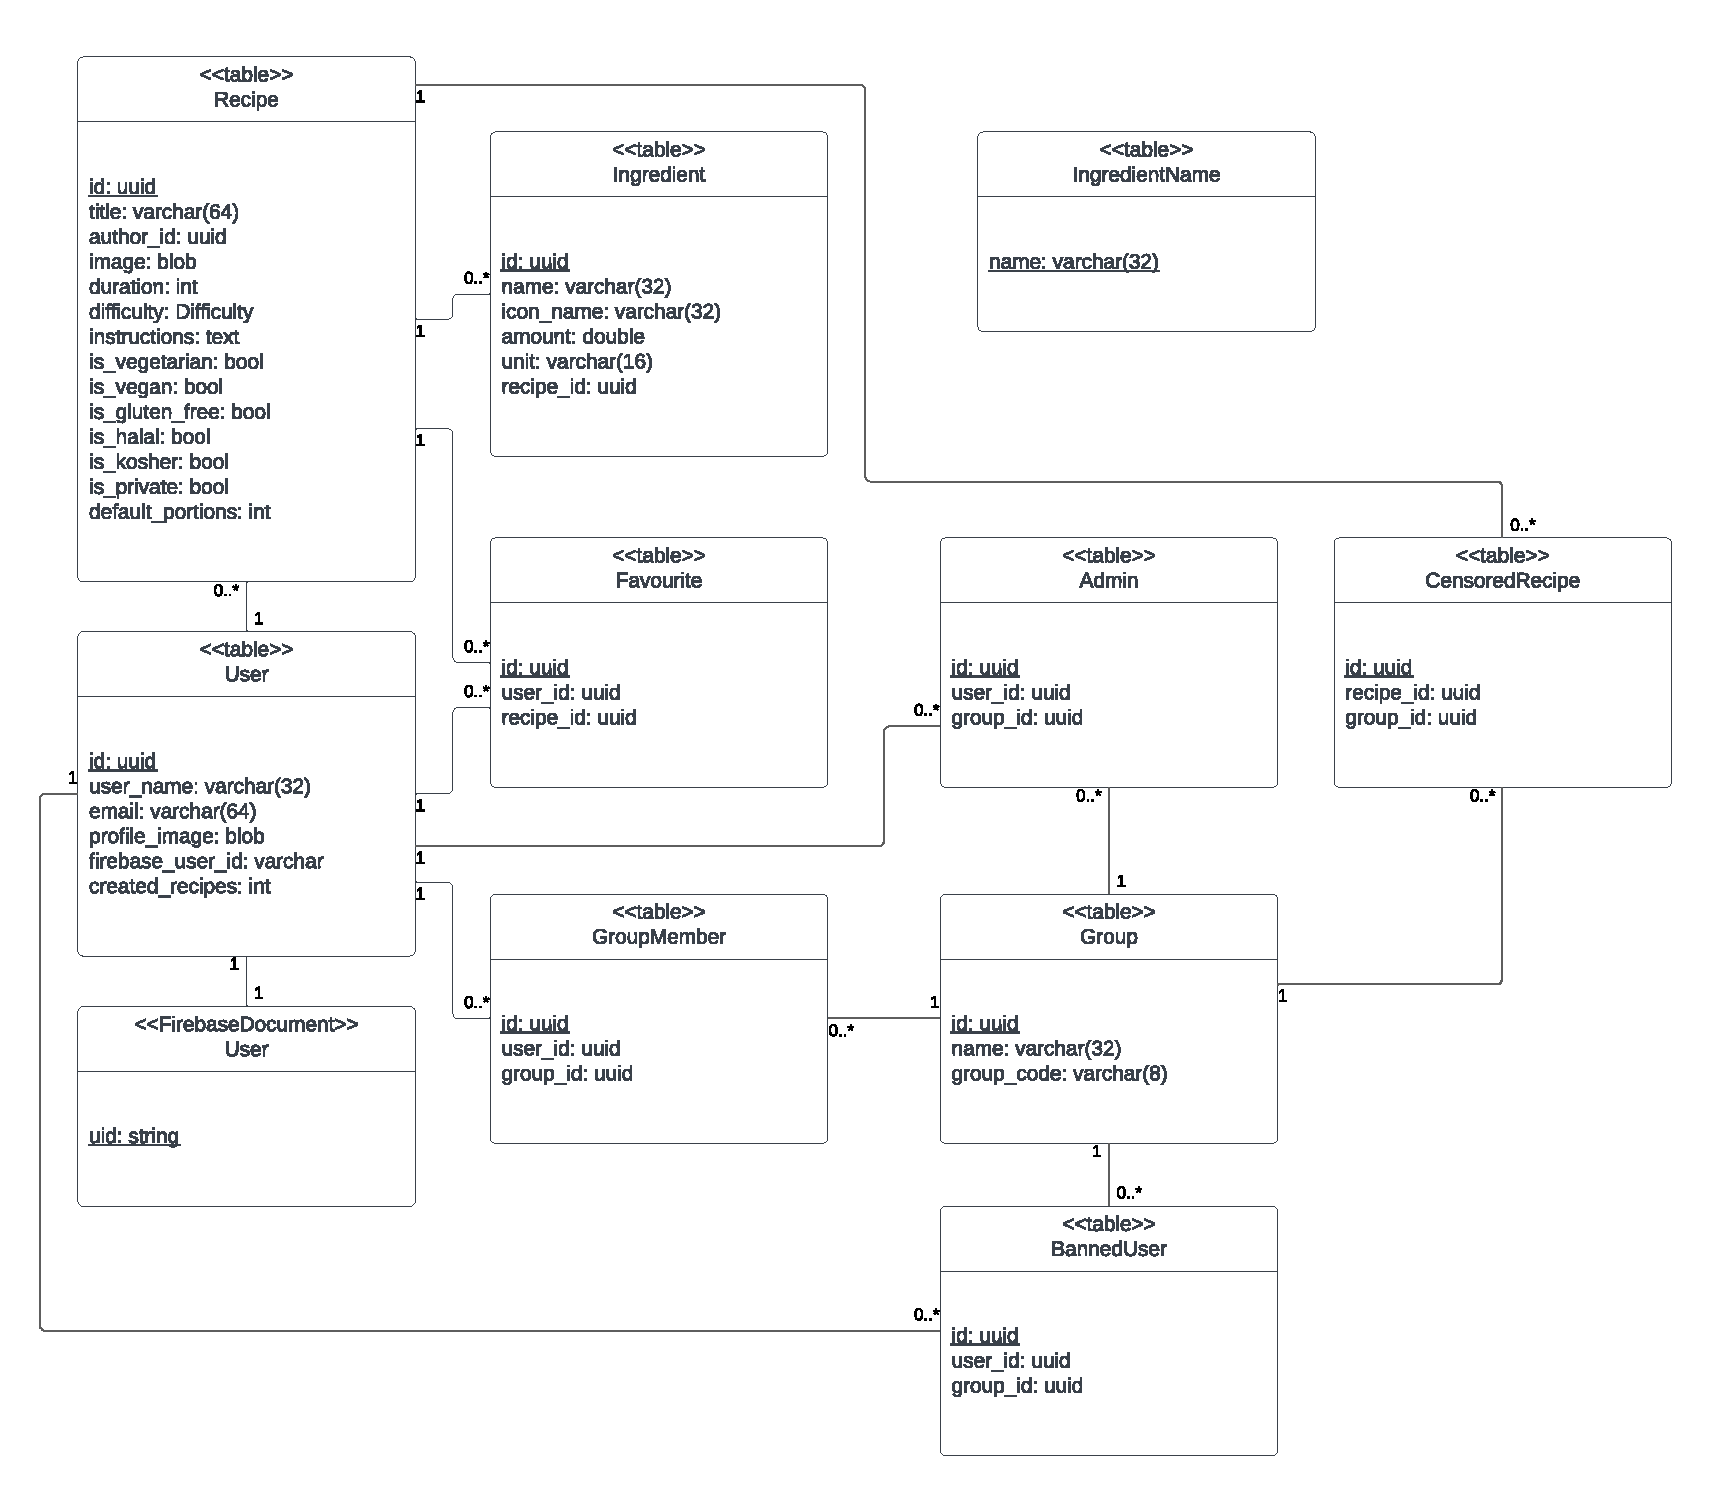
\includegraphics[width = \linewidth]{images/database/databaseSchema.pdf}
    \caption{Datenbankschema}
\end{figure}
Im Datenbankschema werden die einzelnen Entitäten der App abgebildet. Die einzelnen Tabellen werden nun genauer erläutert.
\newpage
\subsubsection{Recipe}
Die Tabelle "Recipe" enthält die Rezepte und besitzt die folgenden Attribute:
\paragraph{\texttt{id (uuid - primary key):}} Die Id stellt den Primärschlüssel des Rezepts dar und muss daher eindeutig und nicht leer sein. Der Datentyp ist \Gls{uuid}. Sie wird automatisch generiert.
\paragraph{\texttt{title (varchar(64) - not null):}} Der Titel des Rezepts. Der Datentyp ist \Gls{varchar}. Er darf nicht leer und maximal 64 Zeichen lang sein.
\paragraph{\texttt{author\_id (uuid - not null, foreign key):}} Hierbei handelt es sich um die Id des Autors des Rezepts als Fremdschlüssel. Sie darf nicht leer sein und der Datentyp ist \Gls{uuid}, da es sich um eine Id handelt.
\paragraph{\texttt{image (blob):}} Das Bild des Rezepts in binär Code. Der Datentyp ist \Gls{blob}.
\paragraph{\texttt{duration (int - not null):}} Die Zubereitungszeit des Rezepts in Minuten. Der Datentyp ist Integer. Sie darf nicht leer sein.
\paragraph{\texttt{difficulty (Difficulty - not null):}} Die Schwierigkeit des Rezepts, die nicht leer sein darf. Der Datentyp "Difficulty" ist ein Enum, mit den Werten "easy", "medium" und "hard".
\paragraph{\texttt{instructions (text - not null):}} Die Zubereitungsanleitung des Rezepts, die nicht leer sein darf. Der Datentyp ist Text, was einer unbegrenzten Zeichenkette entspricht.
\paragraph{\texttt{is\_vegetarian (bool - not null):}} Gibt an, ob das \Gls{label} "Vegetarisch" aktiviert ist. Der Datentyp ist Boolean und darf nicht leer sein.
\paragraph{\texttt{is\_vegan (bool - not null):}} Gibt an, ob das \Gls{label} "Vegan" aktiviert ist. Der Datentyp ist Boolean und darf nicht leer sein.
\paragraph{\texttt{is\_gluten\_free (bool - not null):}} Gibt an, ob das \Gls{label} "Glutenfrei" aktiviert ist. Der Datentyp ist Boolean und darf nicht leer sein.
\paragraph{\texttt{is\_halal (bool - not null):}} Gibt an, ob das \Gls{label} "Halal" aktiviert ist. Der Datentyp ist Boolean und darf nicht leer sein.
\paragraph{\texttt{is\_kosher (bool - not null):}} Gibt an, ob das \Gls{label} "Koscher" aktiviert ist. Der Datentyp ist Boolean und darf nicht leer sein.
\paragraph{\texttt{default\_portions (int - not null):}} Die Anzahl der Portionen, für die das Rezept ausgelegt ist. Der Datentyp ist Integer und darf nicht leer sein. Er wird in der App zur Berechnung der Mengen der Zutaten verwendet.
\newpage
\subsubsection{Ingredient}
Die Tabelle "Ingredient" enthält die Zutaten, die den eizelnen Rezepten zugeordnet sind und besitzt die folgenden Attribute:
\paragraph{\texttt{id (uuid - primary key):}} Die Id stellt den Primärschlüssel der Zutat dar und muss daher eindeutig und nicht leer sein. Der Datentyp ist \Gls{uuid}. Sie wird automatisch generiert.
\paragraph{\texttt{name (varchar(32) - not null):}} Der Name der Zutat. Der Datentyp ist \Gls{varchar}. Er darf nicht leer und maximal 32 Zeichen lang sein.
\paragraph{\texttt{icon\_name (varchar(32))}} Der Name des Icons, das die Zutat repräsentiert. Der Datentyp ist \Gls{varchar}. Er ist maximal 32 Zeichen lang.
\paragraph{\texttt{amount (int - not null):}} Die Menge der Zutat in der jeweiligen Einheit. Sie darf nicht leer sein und der Datentyp ist Integer.
\paragraph{\texttt{unit (varchar(16)):}} Die Einheit der Zutat. Der Datentyp ist \Gls{varchar}. Sie ist maximal 16 Zeichen lang und optional.
\paragraph{\texttt{recipe\_id (uuid - not null, foreign key):}} Hierbei handelt es sich um die Id des Rezepts, zu dem die Zutat gehört, als Fremdschlüssel. Sie darf nicht leer sein und der Datentyp ist \Gls{uuid}, da es sich um eine Id handelt.
\newpage
\subsubsection{IngredientNames}
Die Tabelle "IngredientNames" enthält lediglich die Namen der Zutaten, die in der Vorschlagsliste beim Zutaten erstellen angezeigt werden. Sie besitzt die folgenden Attribute:
\paragraph{\texttt{name (varchar(32) - primary key):}} Der Name der Zutat. Der Datentyp ist \Gls{varchar}. Es handelt sich um den Primärschlüssel und der Name muss daher eindeutig und nicht leer sein.
\newpage
\subsubsection{User}
Die Tabelle "User" enthält die Benutzer der App und besitzt die folgenden Attribute:
\paragraph{\texttt{id (uuid - primary key):}} Die Id stellt den Primärschlüssel des Benutzers dar und muss daher eindeutig und nicht leer sein. Der Datentyp ist \Gls{uuid}. Sie wird automatisch generiert.
\paragraph{\texttt{user\_name (varchar(32) - not null):}} Der Benutzername des Benutzers. Der Datentyp ist \Gls{varchar}. Er darf nicht leer und maximal 32 Zeichen lang sein.
\paragraph{\texttt{email (varchar(64) - not null):}} Die E-Mail-Adresse des Benutzers. Der Datentyp ist \Gls{varchar}. Sie darf nicht leer und maximal 64 Zeichen lang sein.
\paragraph{\texttt{profile\_image (blob):}} Das Profilbild des Benutzers in binär Code. Der Datentyp ist \Gls{blob}.
\paragraph{\texttt{firebase\_user\_id (varchar - not null, unique)}} Die Id des Benutzers, die in der Firebase Datenbank hinterlegt ist. Der Datentyp ist \Gls{varchar}. Sie muss eindeutig und nicht leer sein. Sie dient als Fremdschlüssel über die Datenbank hinweg zu Firebase.
\newpage
\subsubsection{Favourite}
Die Tabelle "Favourite" repräsentiert die Many-To-Many-Beziehung zwischen den Benutzern und den Rezepten, die sie favorisiert haben. Sie besitzt die folgenden Attribute:
\paragraph{\texttt{id (uuid - primary key):}} Die Id stellt den Primärschlüssel der Beziehung dar und muss daher eindeutig und nicht leer sein. Der Datentyp ist \Gls{uuid}. Sie wird automatisch generiert.
\paragraph{\texttt{user\_id (uuid - not null, foreign key):}} Hierbei handelt es sich um die Id des Benutzers, der das Rezept favorisiert hat, als Fremdschlüssel. Sie darf nicht leer sein und der Datentyp ist \Gls{uuid}, da es sich um eine Id handelt.
\paragraph{\texttt{recipe\_id (uuid - not null, foreign key):}} Hierbei handelt es sich um die Id des Rezepts, das favorisiert wurde, als Fremdschlüssel. Sie darf nicht leer sein und der Datentyp ist \Gls{uuid}, da es sich um eine Id handelt.
\newpage
\subsubsection{Group}
Die Tabelle "Group" enthält die Gruppen bzw. Squads und besitzt die folgenden Attribute:
\paragraph{\texttt{id (uuid - primary key):}} Die Id stellt den Primärschlüssel der Gruppe dar und muss daher eindeutig und nicht leer sein. Der Datentyp ist \Gls{uuid}. Sie wird automatisch generiert.
\paragraph{\texttt{name (varchar(32) - not null):}} Der Name der Gruppe. Der Datentyp ist \Gls{varchar}. Er darf nicht leer und maximal 32 Zeichen lang sein.
\newpage
\subsubsection{GroupMember}
Die Tabelle "GroupMember" repräsentiert die Many-To-Many-Beziehung zwischen den Gruppen und den Benutzern, die Mitglied der Gruppe sind. Sie besitzt die folgenden Attribute:
\paragraph{\texttt{id (uuid - primary key):}} Die Id stellt den Primärschlüssel der Beziehung dar und muss daher eindeutig und nicht leer sein. Der Datentyp ist \Gls{uuid}. Sie wird automatisch generiert.
\paragraph{\texttt{user\_id (uuid - not null, foreign key):}} Hierbei handelt es sich um die Id des Benutzers, der Mitglied der Gruppe ist, als Fremdschlüssel. Sie darf nicht leer sein und der Datentyp ist \Gls{uuid}, da es sich um eine Id handelt.
\paragraph{\texttt{group\_id (uuid - not null, foreign key):}} Hierbei handelt es sich um die Id der Gruppe, zu der der Benutzer gehört, als Fremdschlüssel. Sie darf nicht leer sein und der Datentyp ist \Gls{uuid}, da es sich um eine Id handelt.
\newpage
\subsubsection{Admin}
Die Tabelle "Admin" repräsentiert die Many-To-Many-Beziehung zwischen den Gruppen und den Benutzern, die Administratoren der Gruppe sind. Sie besitzt die folgenden Attribute:
\paragraph{\texttt{id (uuid - primary key):}} Die Id stellt den Primärschlüssel der Beziehung dar und muss daher eindeutig und nicht leer sein. Der Datentyp ist \Gls{uuid}. Sie wird automatisch generiert.
\paragraph{\texttt{user\_id (uuid - not null, foreign key):}} Hierbei handelt es sich um die Id des Benutzers, der Administrator der Gruppe ist, als Fremdschlüssel. Sie darf nicht leer sein und der Datentyp ist \Gls{uuid}, da es sich um eine Id handelt.
\paragraph{\texttt{group\_id (uuid - not null, foreign key):}} Hierbei handelt es sich um die Id der Gruppe, zu der der Benutzer gehört, als Fremdschlüssel. Sie darf nicht leer sein und der Datentyp ist \Gls{uuid}, da es sich um eine Id handelt.
\newpage
\subsubsection{CensoredRecipe}
Die Tabelle "CensoredRecipe" repräsentiert die Many-To-Many-Beziehung zwischen den Gruppen und den Rezepten, die die jeweiligen Administratoren zensiert haben. Sie besitzt die folgenden Attribute:
\paragraph{\texttt{id (uuid - primary key):}} Die Id stellt den Primärschlüssel der Beziehung dar und muss daher eindeutig und nicht leer sein. Der Datentyp ist \Gls{uuid}. Sie wird automatisch generiert.
\paragraph{\texttt{recipe\_id (uuid - not null, foreign key):}} Hierbei handelt es sich um die Id des Rezepts, das zensiert wurde, als Fremdschlüssel. Sie darf nicht leer sein und der Datentyp ist \Gls{uuid}, da es sich um eine Id handelt.
\paragraph{\texttt{group\_id (uuid - not null, foreign key):}} Hierbei handelt es sich um die Id der Gruppe, zu der der Administrator gehört, als Fremdschlüssel. Sie darf nicht leer sein und der Datentyp ist \Gls{uuid}, da es sich um eine Id handelt.
\newpage

\subsubsection{BannedUser}
Die Tabelle "BannedUser" repräsentiert die Many-To-Many-Beziehung zwischen den Gruppen und den Benutzern, die von den jeweiligen Administratoren aus der Gruppe verbannt wurden. Sie besitzt die folgenden Attribute:
\paragraph{\texttt{id (uuid - primary key):}} Die Id stellt den Primärschlüssel der Beziehung dar und muss daher eindeutig und nicht leer sein. Der Datentyp ist \Gls{uuid}. Sie wird automatisch generiert.
\paragraph{\texttt{user\_id (uuid - not null, foreign key):}} Hierbei handelt es sich um die Id des Benutzers, der verbannt wurde, als Fremdschlüssel. Sie darf nicht leer sein und der Datentyp ist \Gls{uuid}, da es sich um eine Id handelt.
\paragraph{\texttt{group\_id (uuid - not null, foreign key):}} Hierbei handelt es sich um die Id der Gruppe, zu der der Administrator gehört, als Fremdschlüssel. Sie darf nicht leer sein und der Datentyp ist \Gls{uuid}, da es sich um eine Id handelt.
\newpage

\section{Ablaufbeschreibung}

\newpage
\section{Klassenindex}
\subsection{Client-Klassen}
\begin{multicols}{2}
    \begin{itemize}[label={}]
        \item \nameref{sec:AddIngredientPage}
        \item \nameref{sec:AddIngredientPageState}
        \item \nameref{sec:AppBar}
        \item \nameref{sec:ConfirmationElement}
        \item \nameref{sec:Difficulty}
        \item \nameref{sec:FilteringMethods}
        \item \nameref{sec:GroupCreationPage}
        \item \nameref{sec:GroupCreationPageState}
        \item \nameref{sec:GroupDetailPage}
        \item \nameref{sec:GroupJoiningPage}
        \item \nameref{sec:GroupJoiningPageState}
        \item \nameref{sec:GroupRepository}
        \item \nameref{sec:GroupService}
        \item \nameref{sec:GroupMember}
        \item \nameref{sec:GroupRecipe}
        \item \nameref{sec:InformationCategories}
        \item \nameref{sec:InformationElement}
        \item \nameref{sec:ingredient}
        \item \nameref{sec:LoginPagePage}
        \item \nameref{sec:LoginPageState}
        \item \nameref{sec:LogoutButton}
        \item \nameref{sec:LocalRecipeRepository}
        \item \nameref{sec:MainViewPage}
        \item \nameref{sec:MainViewPageState}
        \item \nameref{sec:OptionElement}
        \item \nameref{sec:PdfExporter}
        \item \nameref{sec:QrCodePage}
        \item \nameref{sec:Recipe}
        \item \nameref{sec:RecipeCreationPage}
        \item \nameref{sec:RecipeCreationPageState}
        \item \nameref{sec:RecipeElement}
        \item \nameref{sec:RecipeService}
        \item \nameref{sec:RecipeViewPage}
        \item \nameref{sec:RecipeViewPageState}
        \item \nameref{sec:RegisterPage}
        \item \nameref{sec:RegisterPageState}
        \item \nameref{sec:RemoteRecipeRepository}
        \item \nameref{sec:ResetPasswordPage}
        \item \nameref{sec:ResetPasswordPageState}
        \item \nameref{sec:ReturnButton}
        \item \nameref{sec:SettingsPage}
        \item \nameref{sec:SettingsPageState}
        \item \nameref{sec:SortingMethods}
        \item \nameref{sec:TopBar}
        \item \nameref{sec:User}
        \item \nameref{sec:UserElement}
        \item \nameref{sec:UserRepository}
        \item \nameref{sec:UserService}
    \end{itemize}
\end{multicols}
\subsection{Server-Klassen}
\begin{multicols}{2}
    \begin{itemize}[label={}]
        \item \nameref{sec:AbstractController}
        \item \nameref{sec:AbstractRouter}
        \item \nameref{sec:AdminUserController}
        \item \nameref{sec:AdminUserRouter}
        \item \nameref{sec:Application}
        \item \nameref{sec:AuthentificationController}
        \item \nameref{sec:AuthentificationRouter}
        \item \nameref{sec:GroupController}
        \item \nameref{sec:GroupRouter}
        \item \nameref{sec:IngredientController}
        \item \nameref{sec:IngredientRouter}
        \item \nameref{sec:RecipeController}
        \item \nameref{sec:RecipeRouter}
        \item \nameref{sec:Server}
        \item \nameref{sec:UserRouter} 
        \item \nameref{sec:UserController}
    \end{itemize}
\end{multicols}
\newpage
\section{Glossar}
\printglossary[style=altlist]
\end{document}